\begin{appendices}    
    
\chapter{Data/MC Checks} \label{app:data_mc_checks}

This section shows the plots made to check whether the distributions of the input variables agree between data and simulations.

\begin{figure}[h]
    \centering
    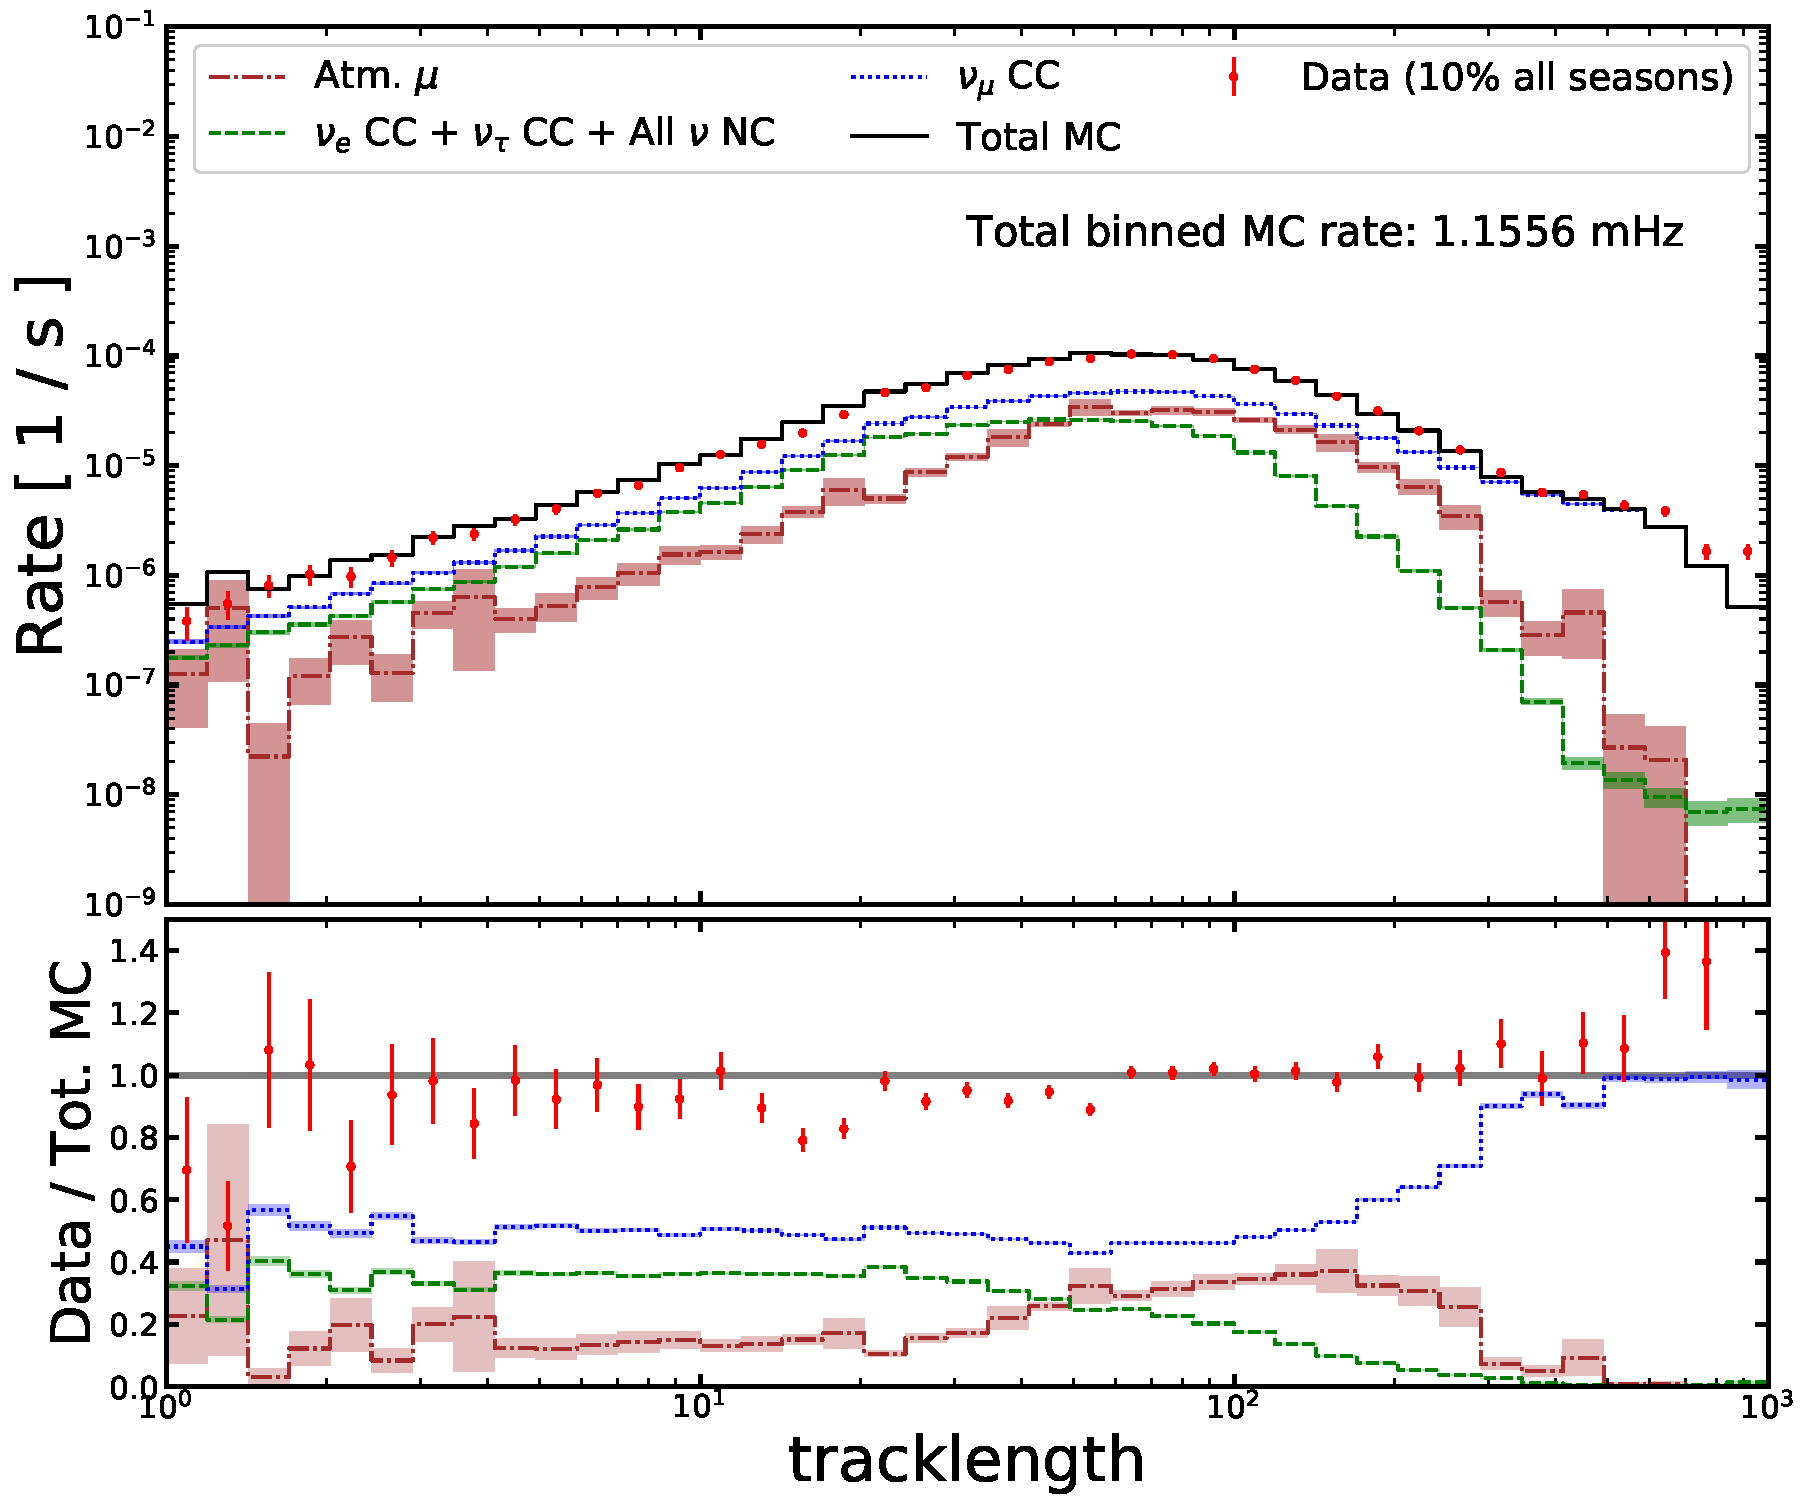
\includegraphics[width=0.75\linewidth]{figures/L7_SANTA_classifier_length_14_bigger.pdf}
    \caption[The simulated distribution of track length compared to 10\,\% of the OscNext data sample]{The simulated distributions of track length compared to 10\,\% of the OscNext data sample (red points). Shown are the contributions from atmospheric muons (dark red), track-like events (blue), cascade-like events (green) and the combined simulation in black.}
    \label{fig:data_mc_tracklength}
\end{figure}

\begin{figure}[h]
	\centering
    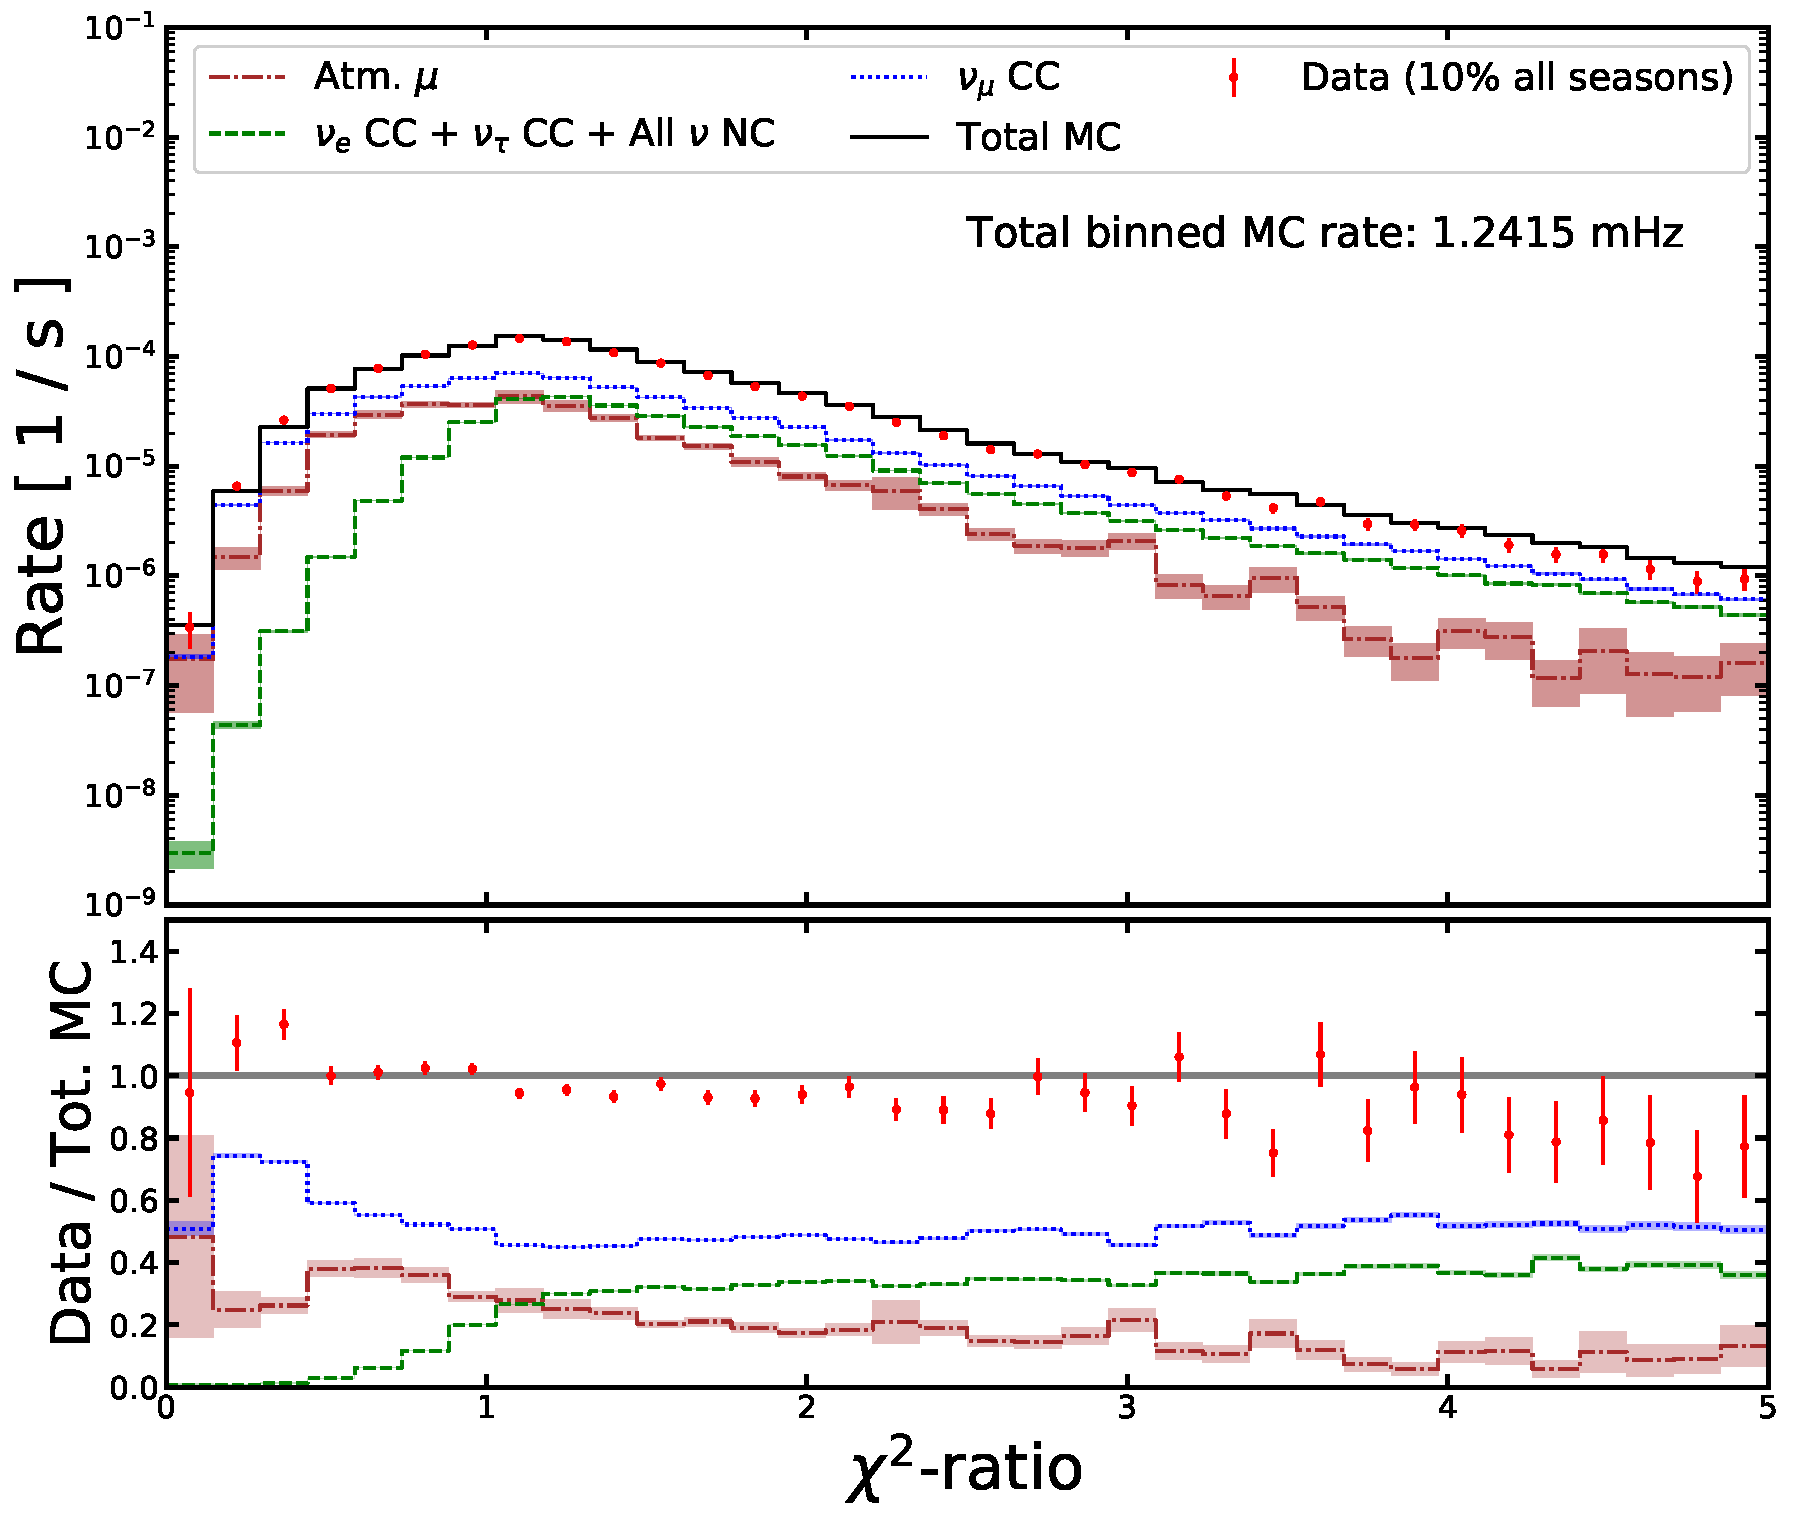
\includegraphics[width=0.75\linewidth]{figures/L7_SANTA_classifier_santapid_14_bigger.pdf}
    
    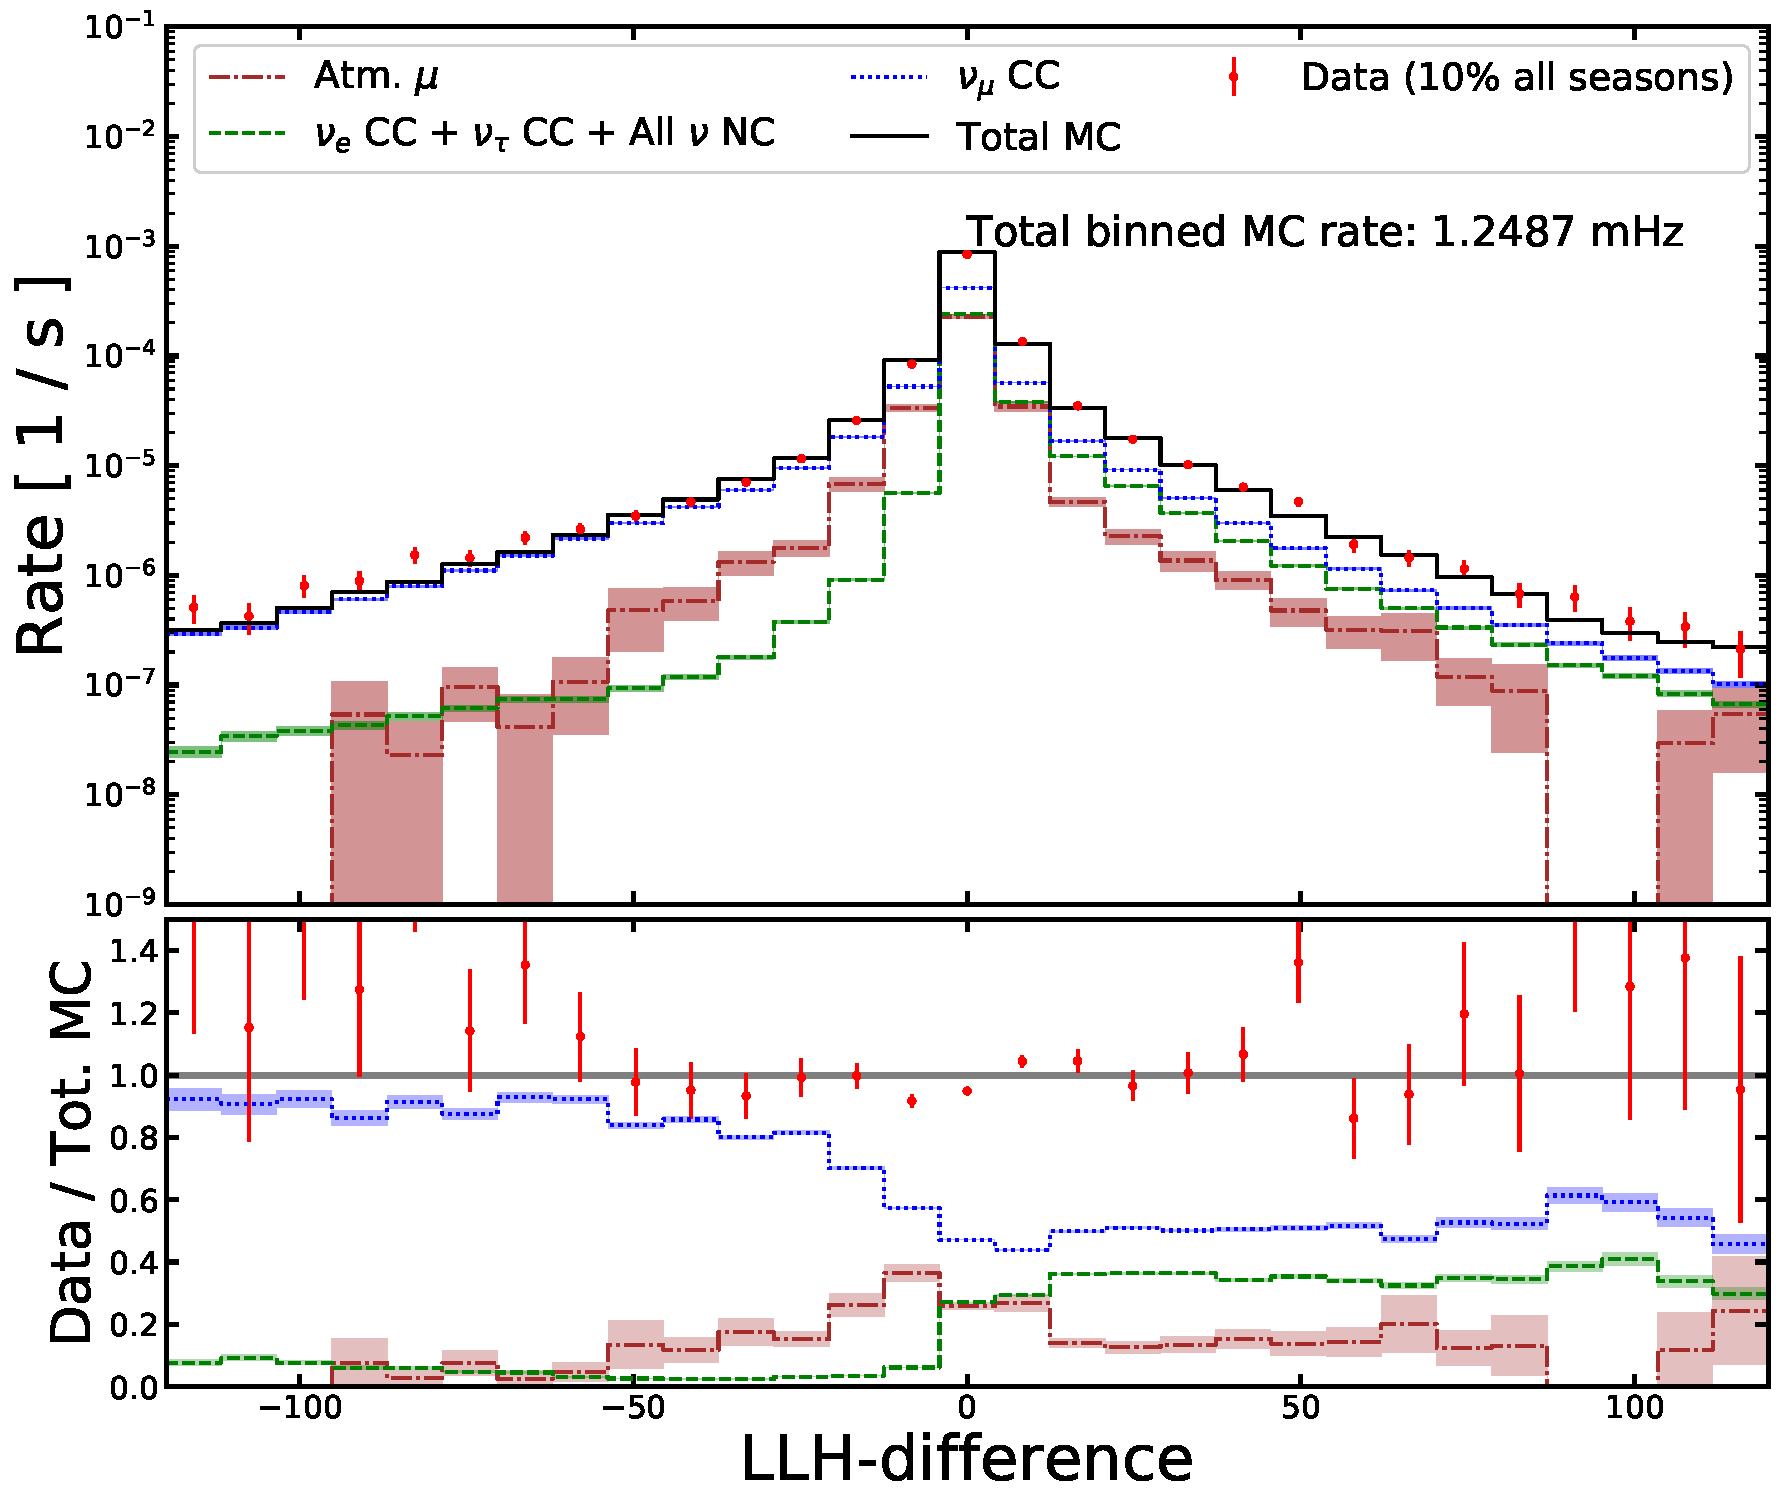
\includegraphics[width=0.75\linewidth]{figures/L7_SANTA_classifier_leerapid_14_bigger.pdf}
    \caption[The simulated distributions of $\chi^2$-ratio (left) and LLH-difference (right) compared to 10\,\% of the OscNext data sample]{The simulated distributions of $\chi^2$-ratio (left) and LLH-difference (right) compared to 10\,\% of the OscNext data sample (red points). Shown are the contributions from atmospheric muons (dark red), track-like events (blue), cascade-like events (green) and the combined simulation in black.}
    \label{fig:data_mc_chi2_llhdiff}
\end{figure}

\begin{figure}[h]
	\centering
    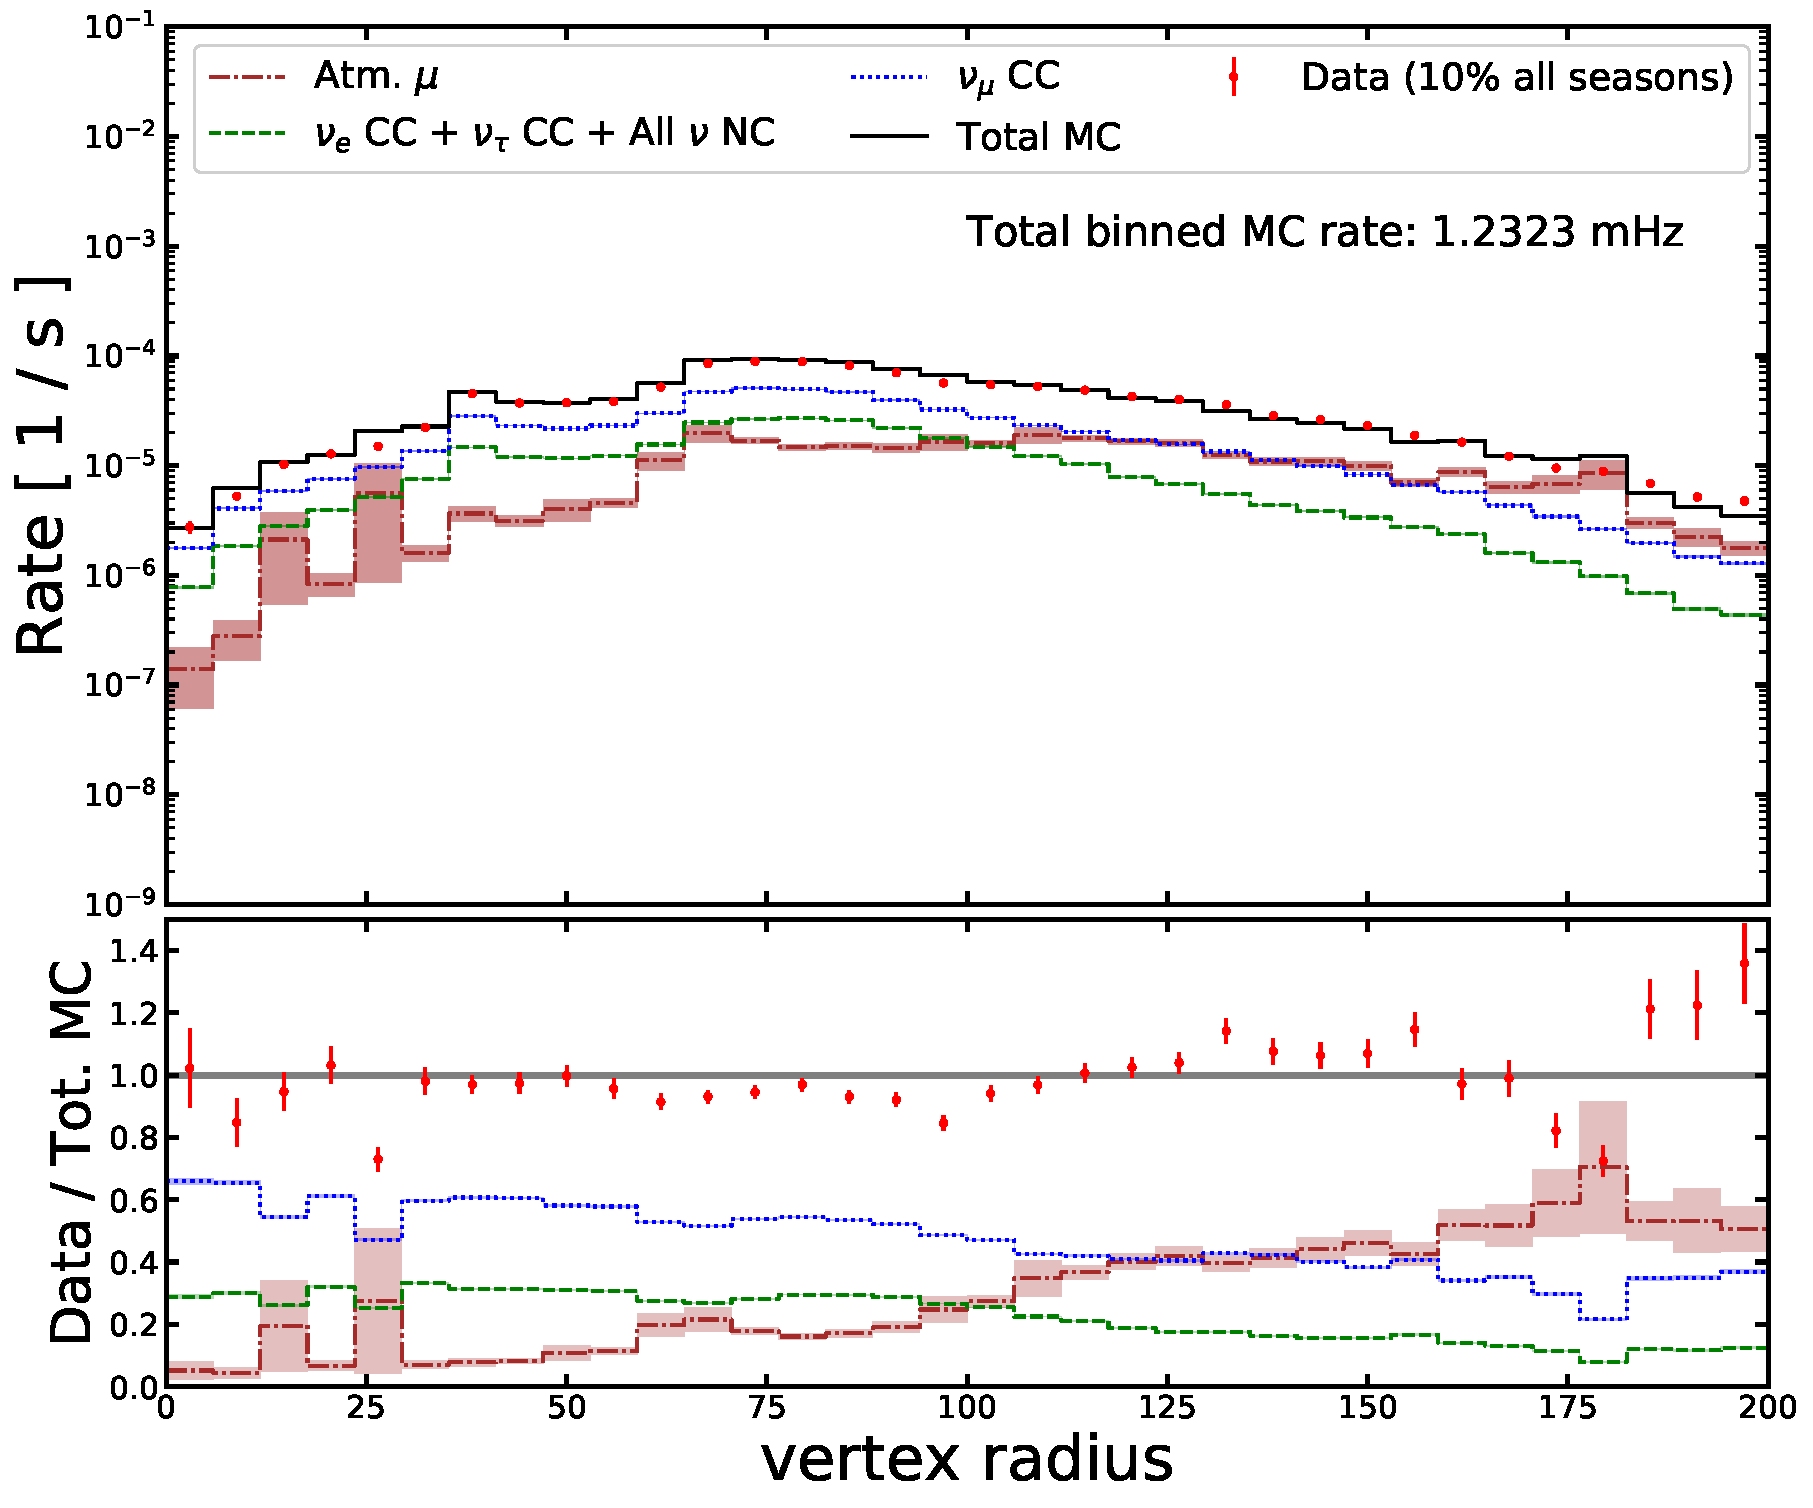
\includegraphics[width=0.75\linewidth]{figures/L7_SANTA_classifier_rho36start_14_bigger.pdf}
    
    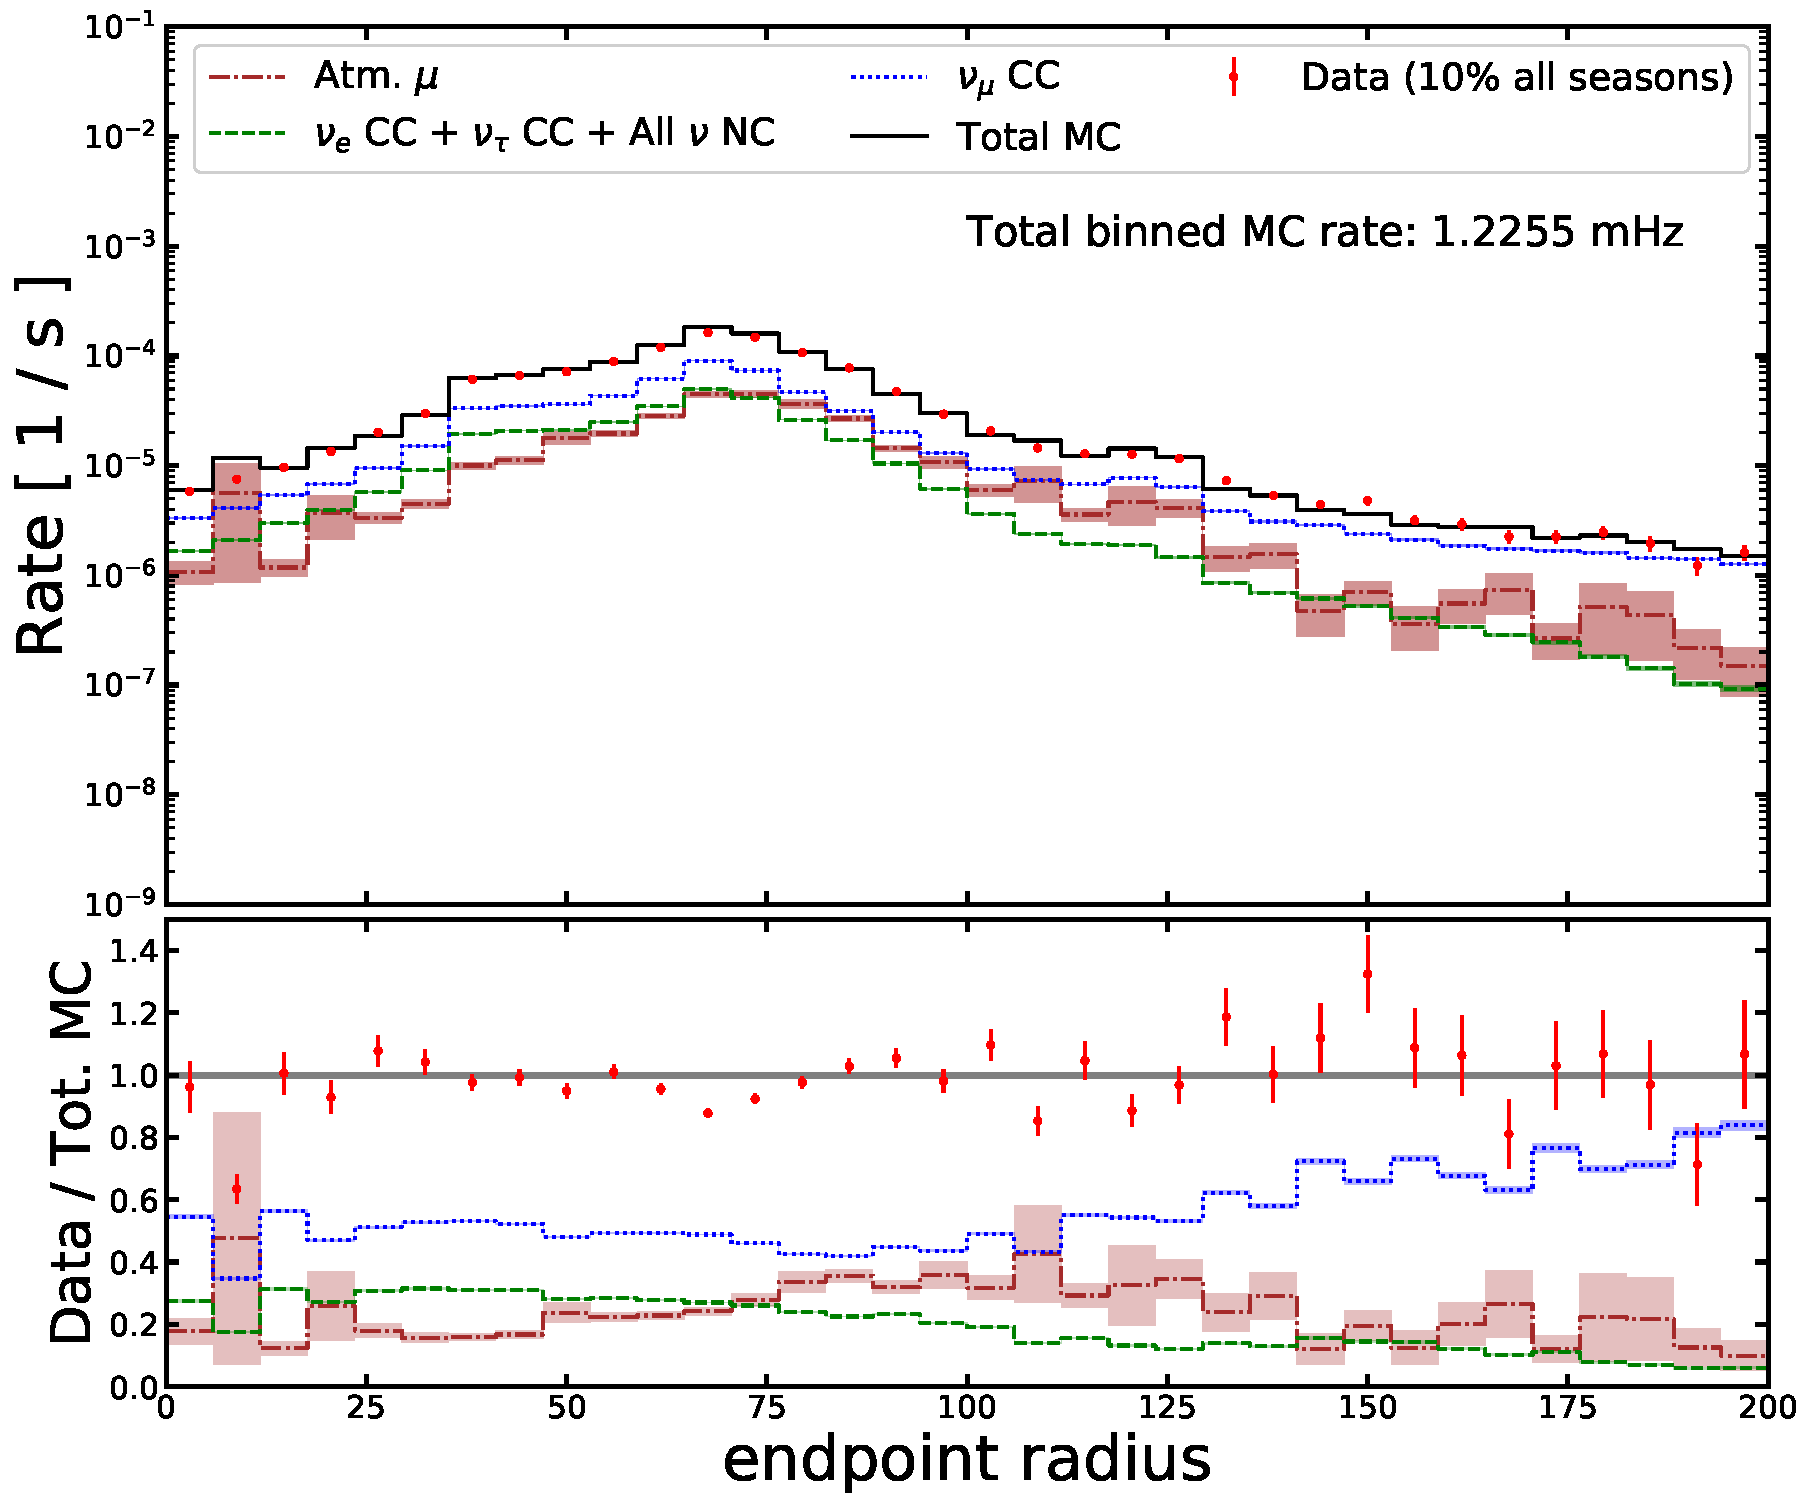
\includegraphics[width=0.75\linewidth]{figures/L7_SANTA_classifier_rho36end_14_bigger.pdf}
    \caption[The simulated distributions of vertex radius (left) and endpoint radius (right) compared to 10\,\% of the OscNext data sample]{The simulated distributions of vertex radius (left) and endpoint radius (right) compared to 10\,\% of the OscNext data sample (red points). Shown are the contributions from atmospheric muons (dark red), track-like events (blue), cascade-like events (green) and the combined simulation in black.}
    \label{fig:data_mc_rstart_rend}
\end{figure}

\begin{figure}[h]
	\centering
    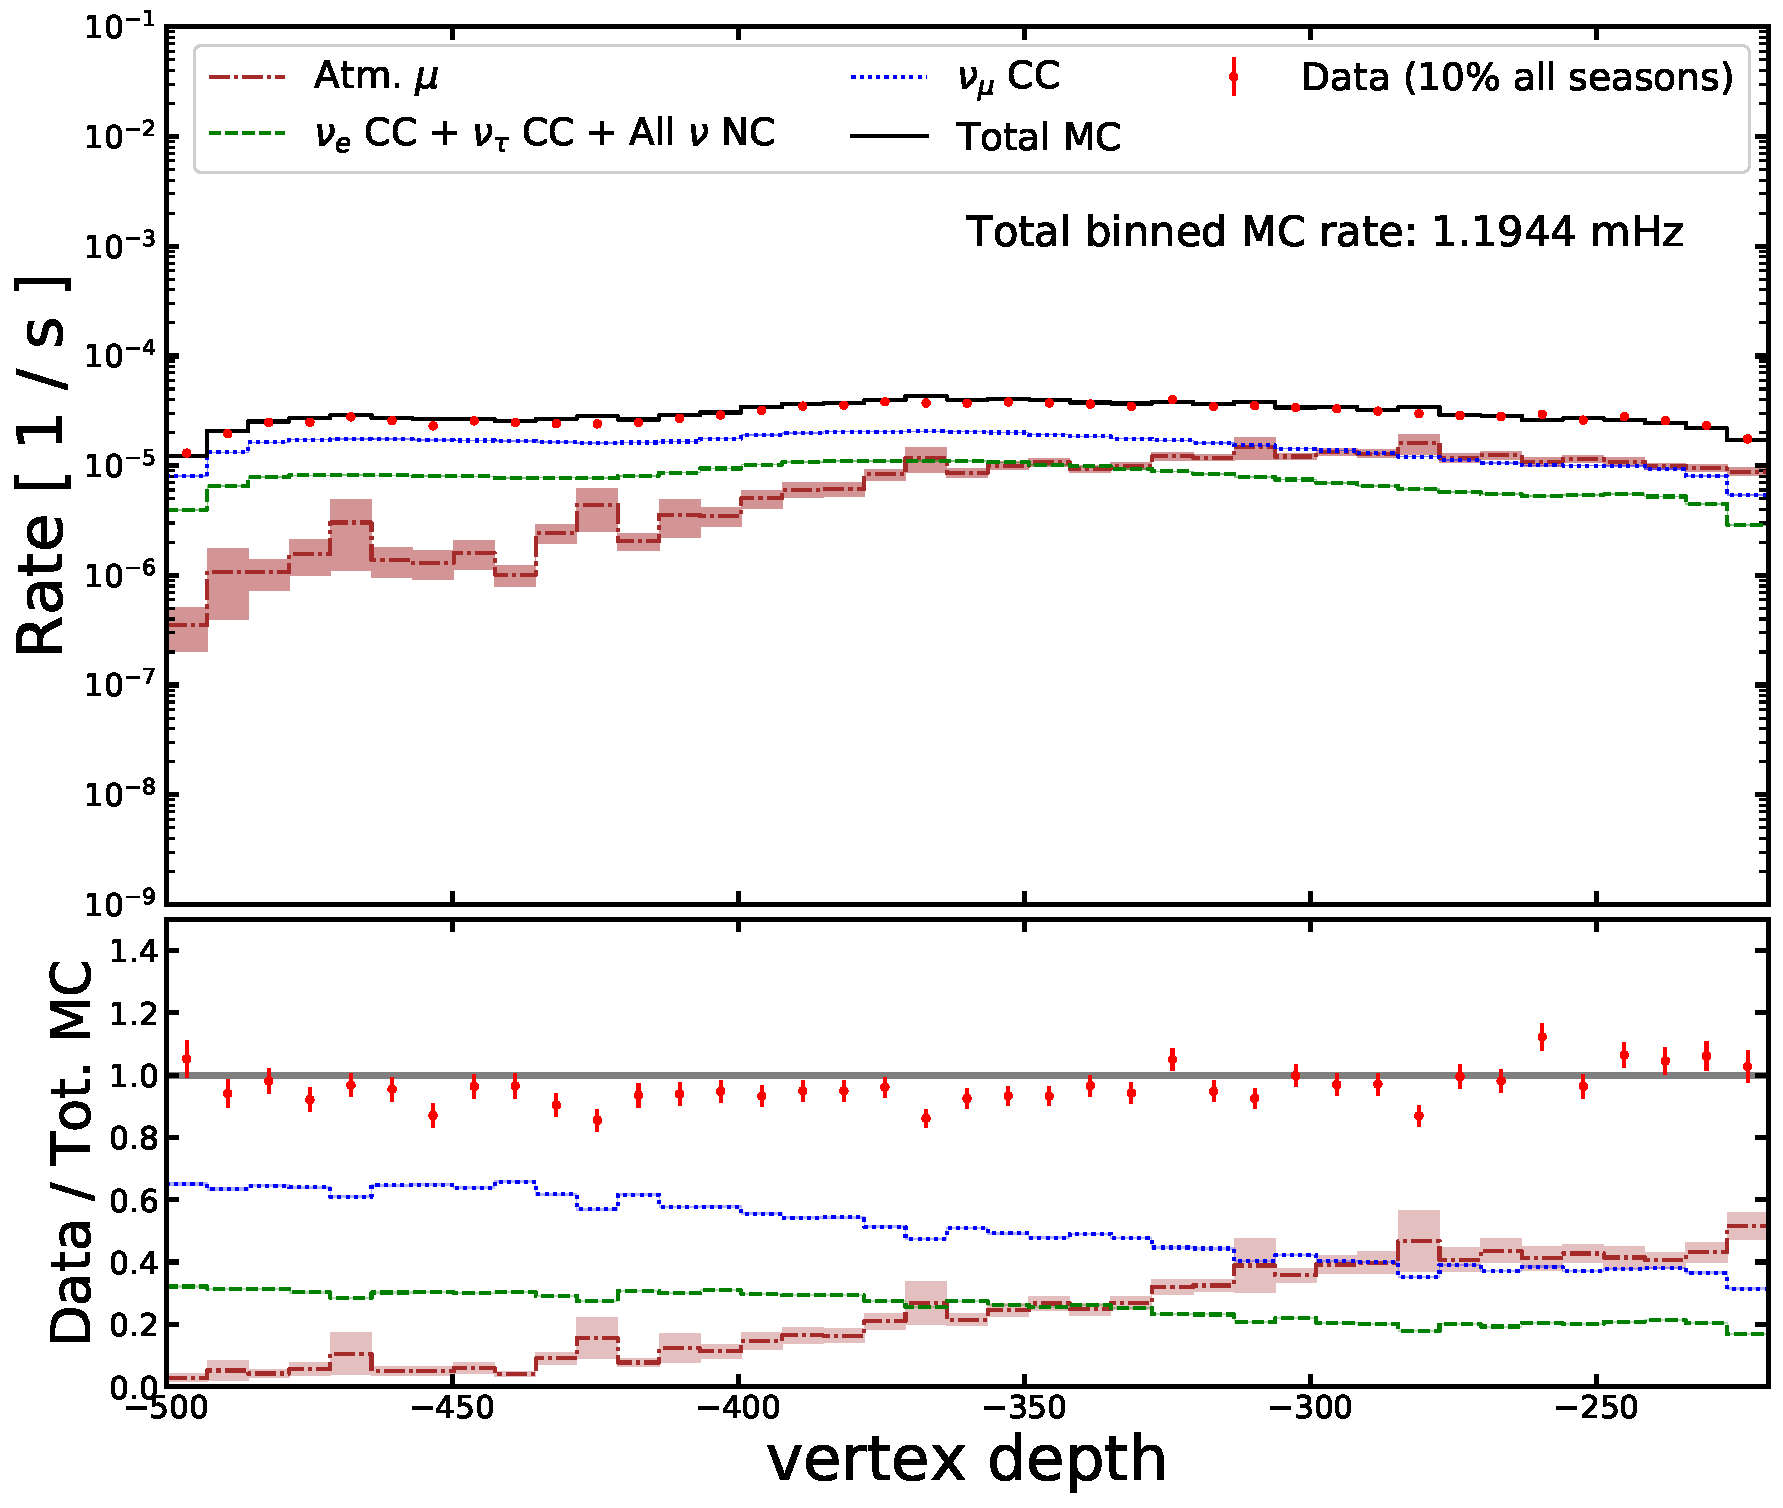
\includegraphics[width=0.75\linewidth]{figures/L7_SANTA_classifier_zstart_14_bigger.pdf}
    
    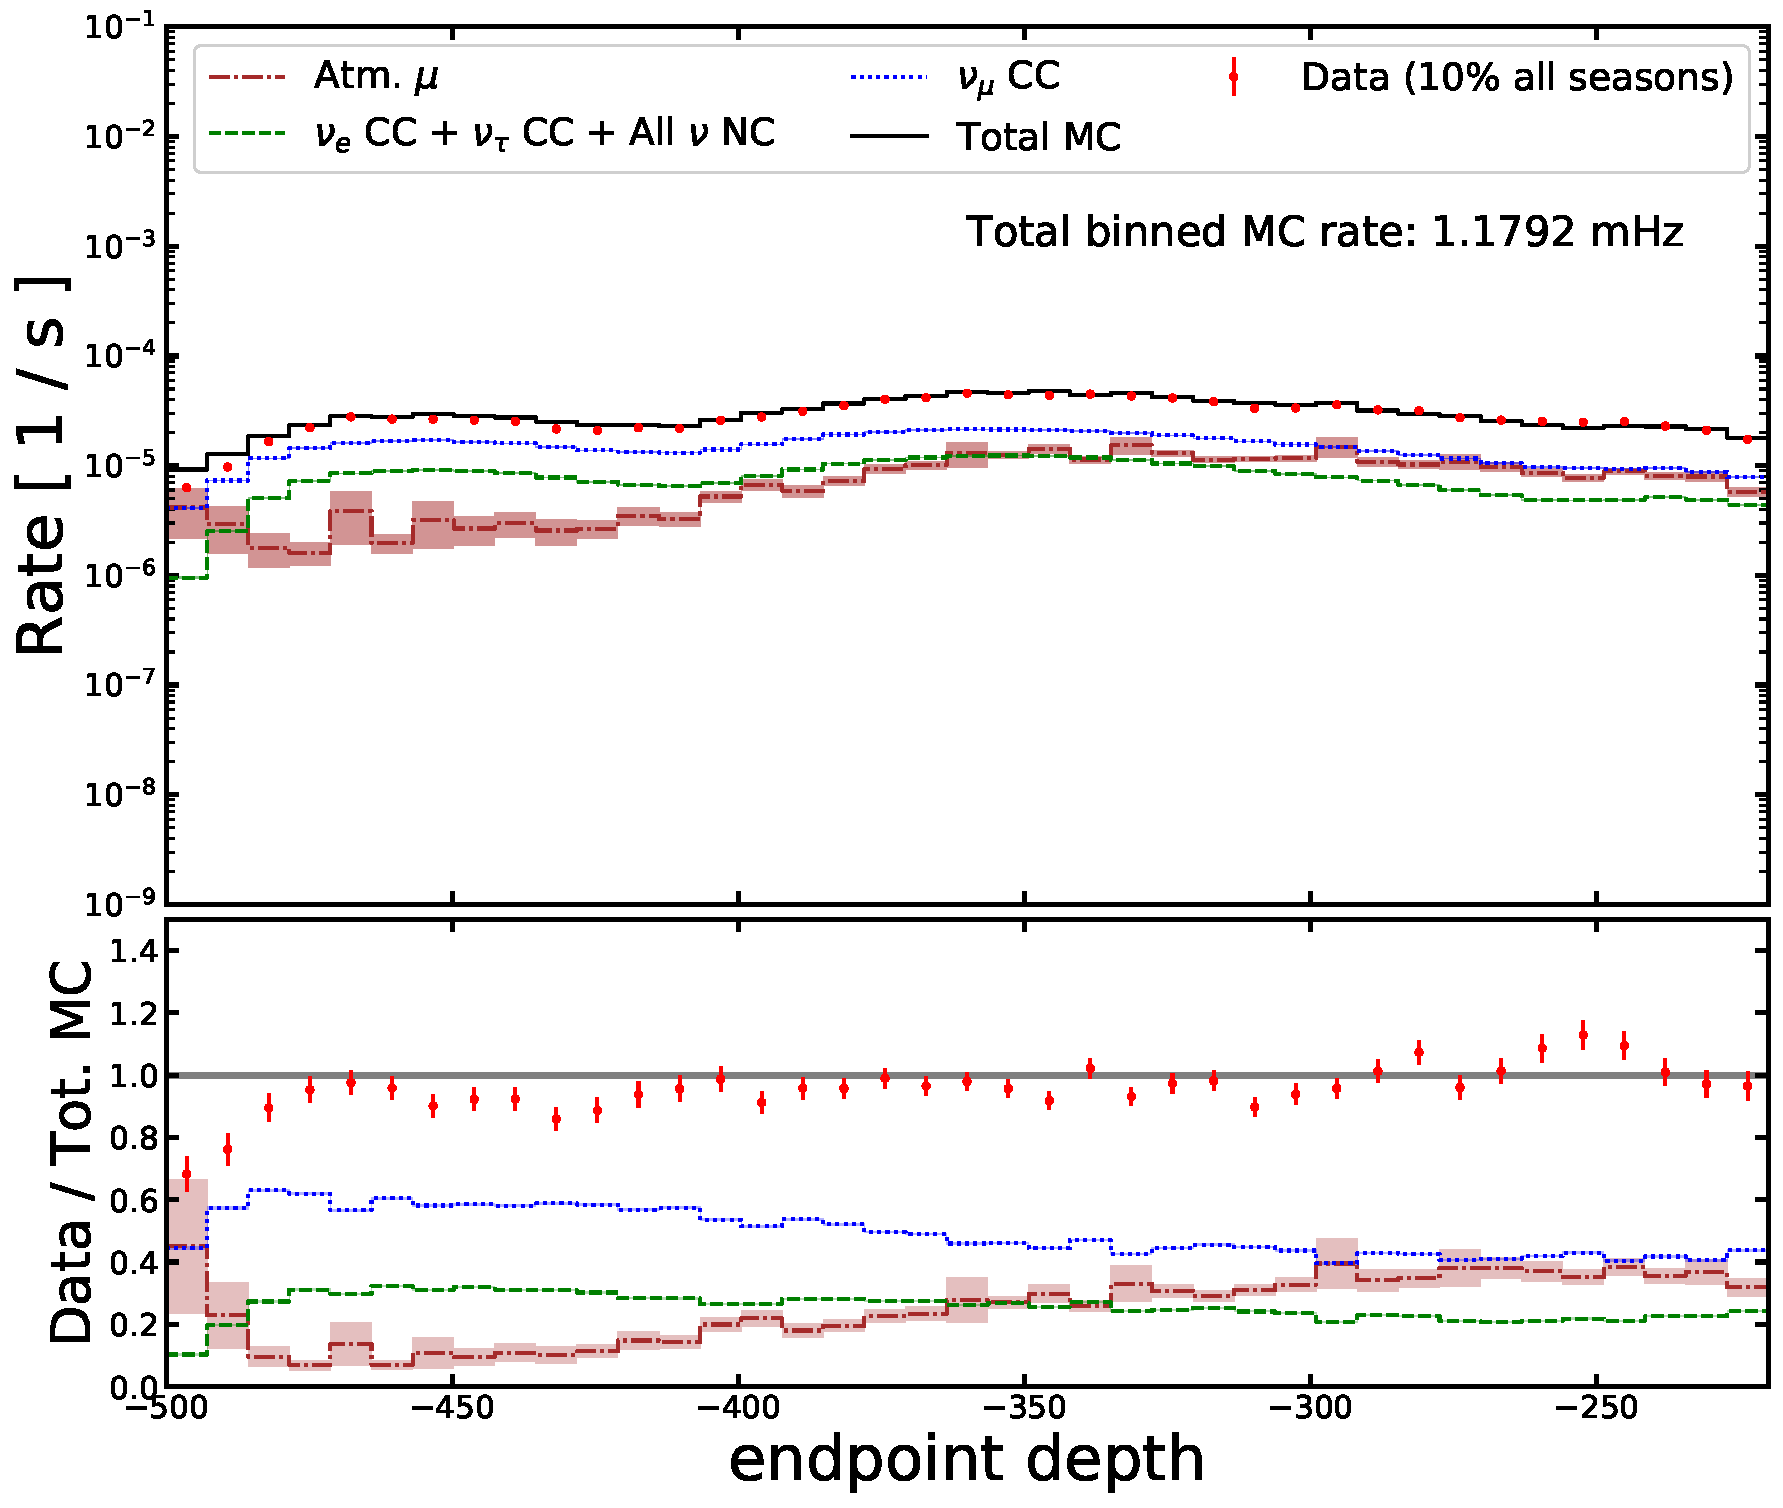
\includegraphics[width=0.75\linewidth]{figures/L7_SANTA_classifier_zend_14_bigger.pdf}
    \caption[The simulated distributions of vertex depth (left) and endpoint depth (right) compared to 10\,\% of the OscNext data sample]{The simulated distributions of vertex depth (left) and endpoint depth (right) compared to 10\,\% of the OscNext data sample (red points). Shown are the contributions from atmospheric muons (dark red), track-like events (blue), cascade-like events (green) and the combined simulation in black.}
    \label{fig:data_mc_zstart_zend}
\end{figure}


\chapter{Expected Event Distributions} \label{app:event_distributions}

This section shows the expected histograms with the event rates with and without oscillations for the different PID bins.
% Shown are the expected event rates with and without oscillation.
%  and the ratio between oscillated and unoscillated.

\begin{figure}[h]
    \centering
    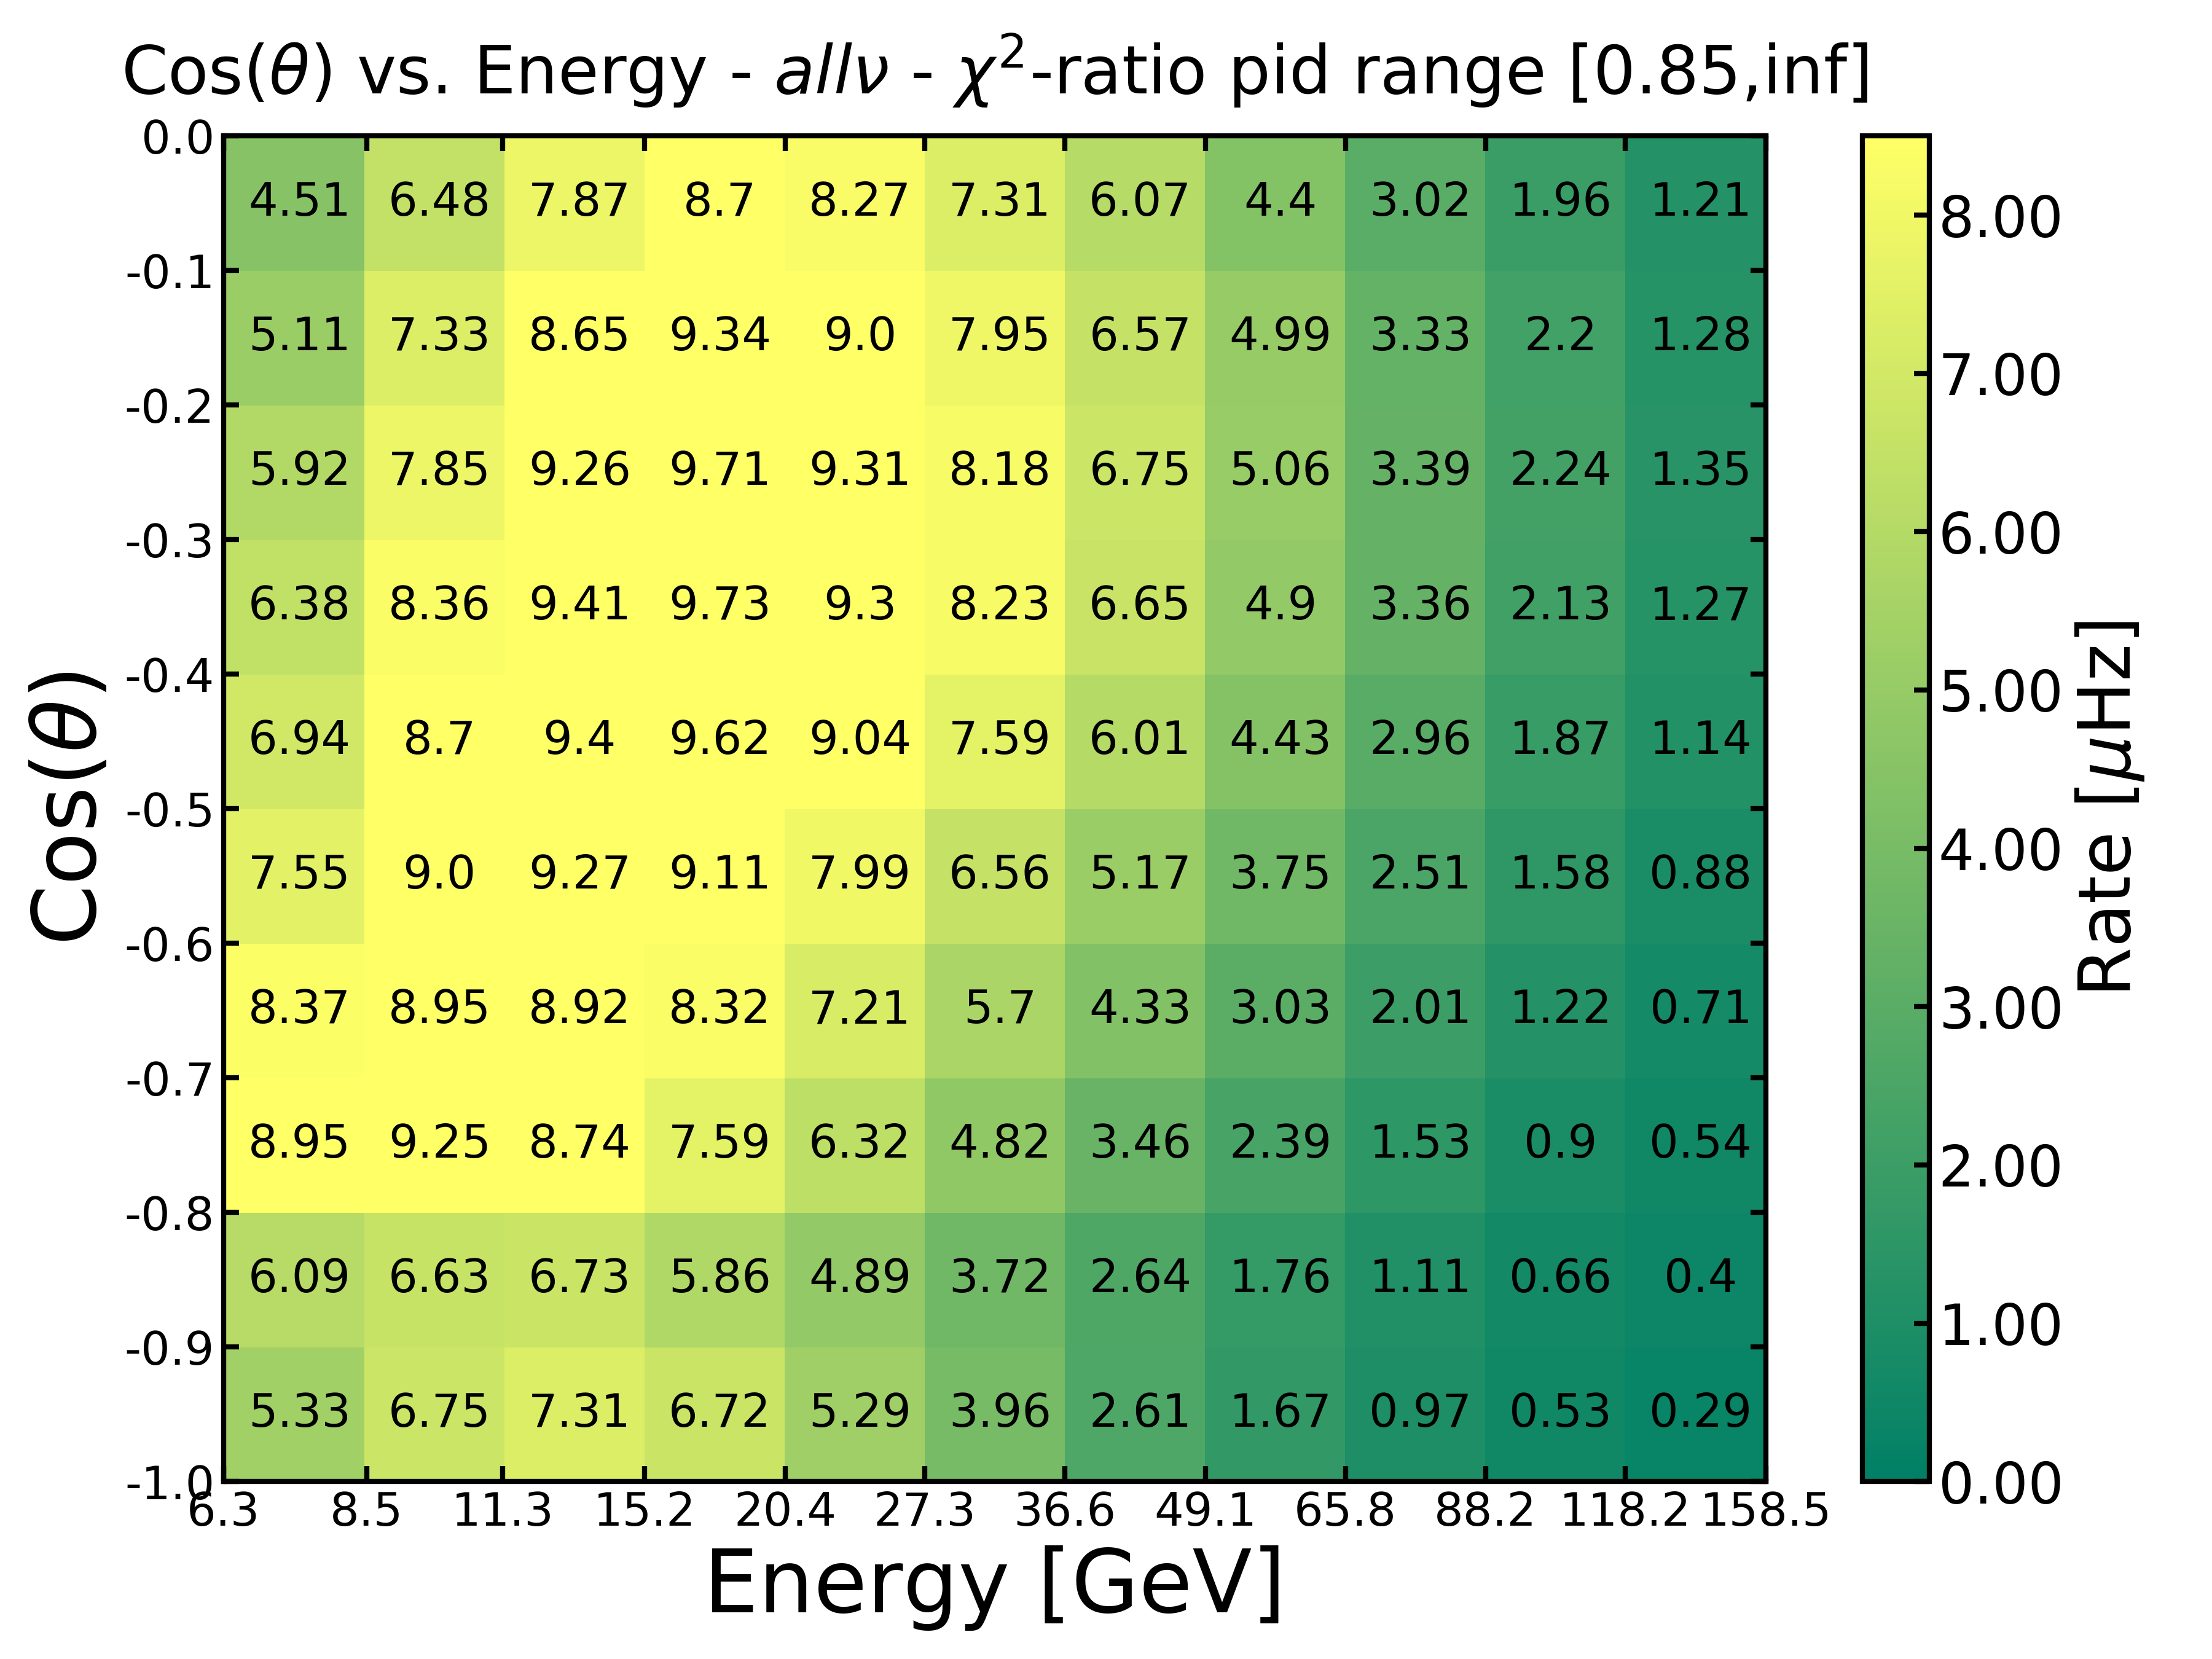
\includegraphics[width=0.49\linewidth]{figures/santa_cut_085_allnu_1_unoscillated_vmax.png}
    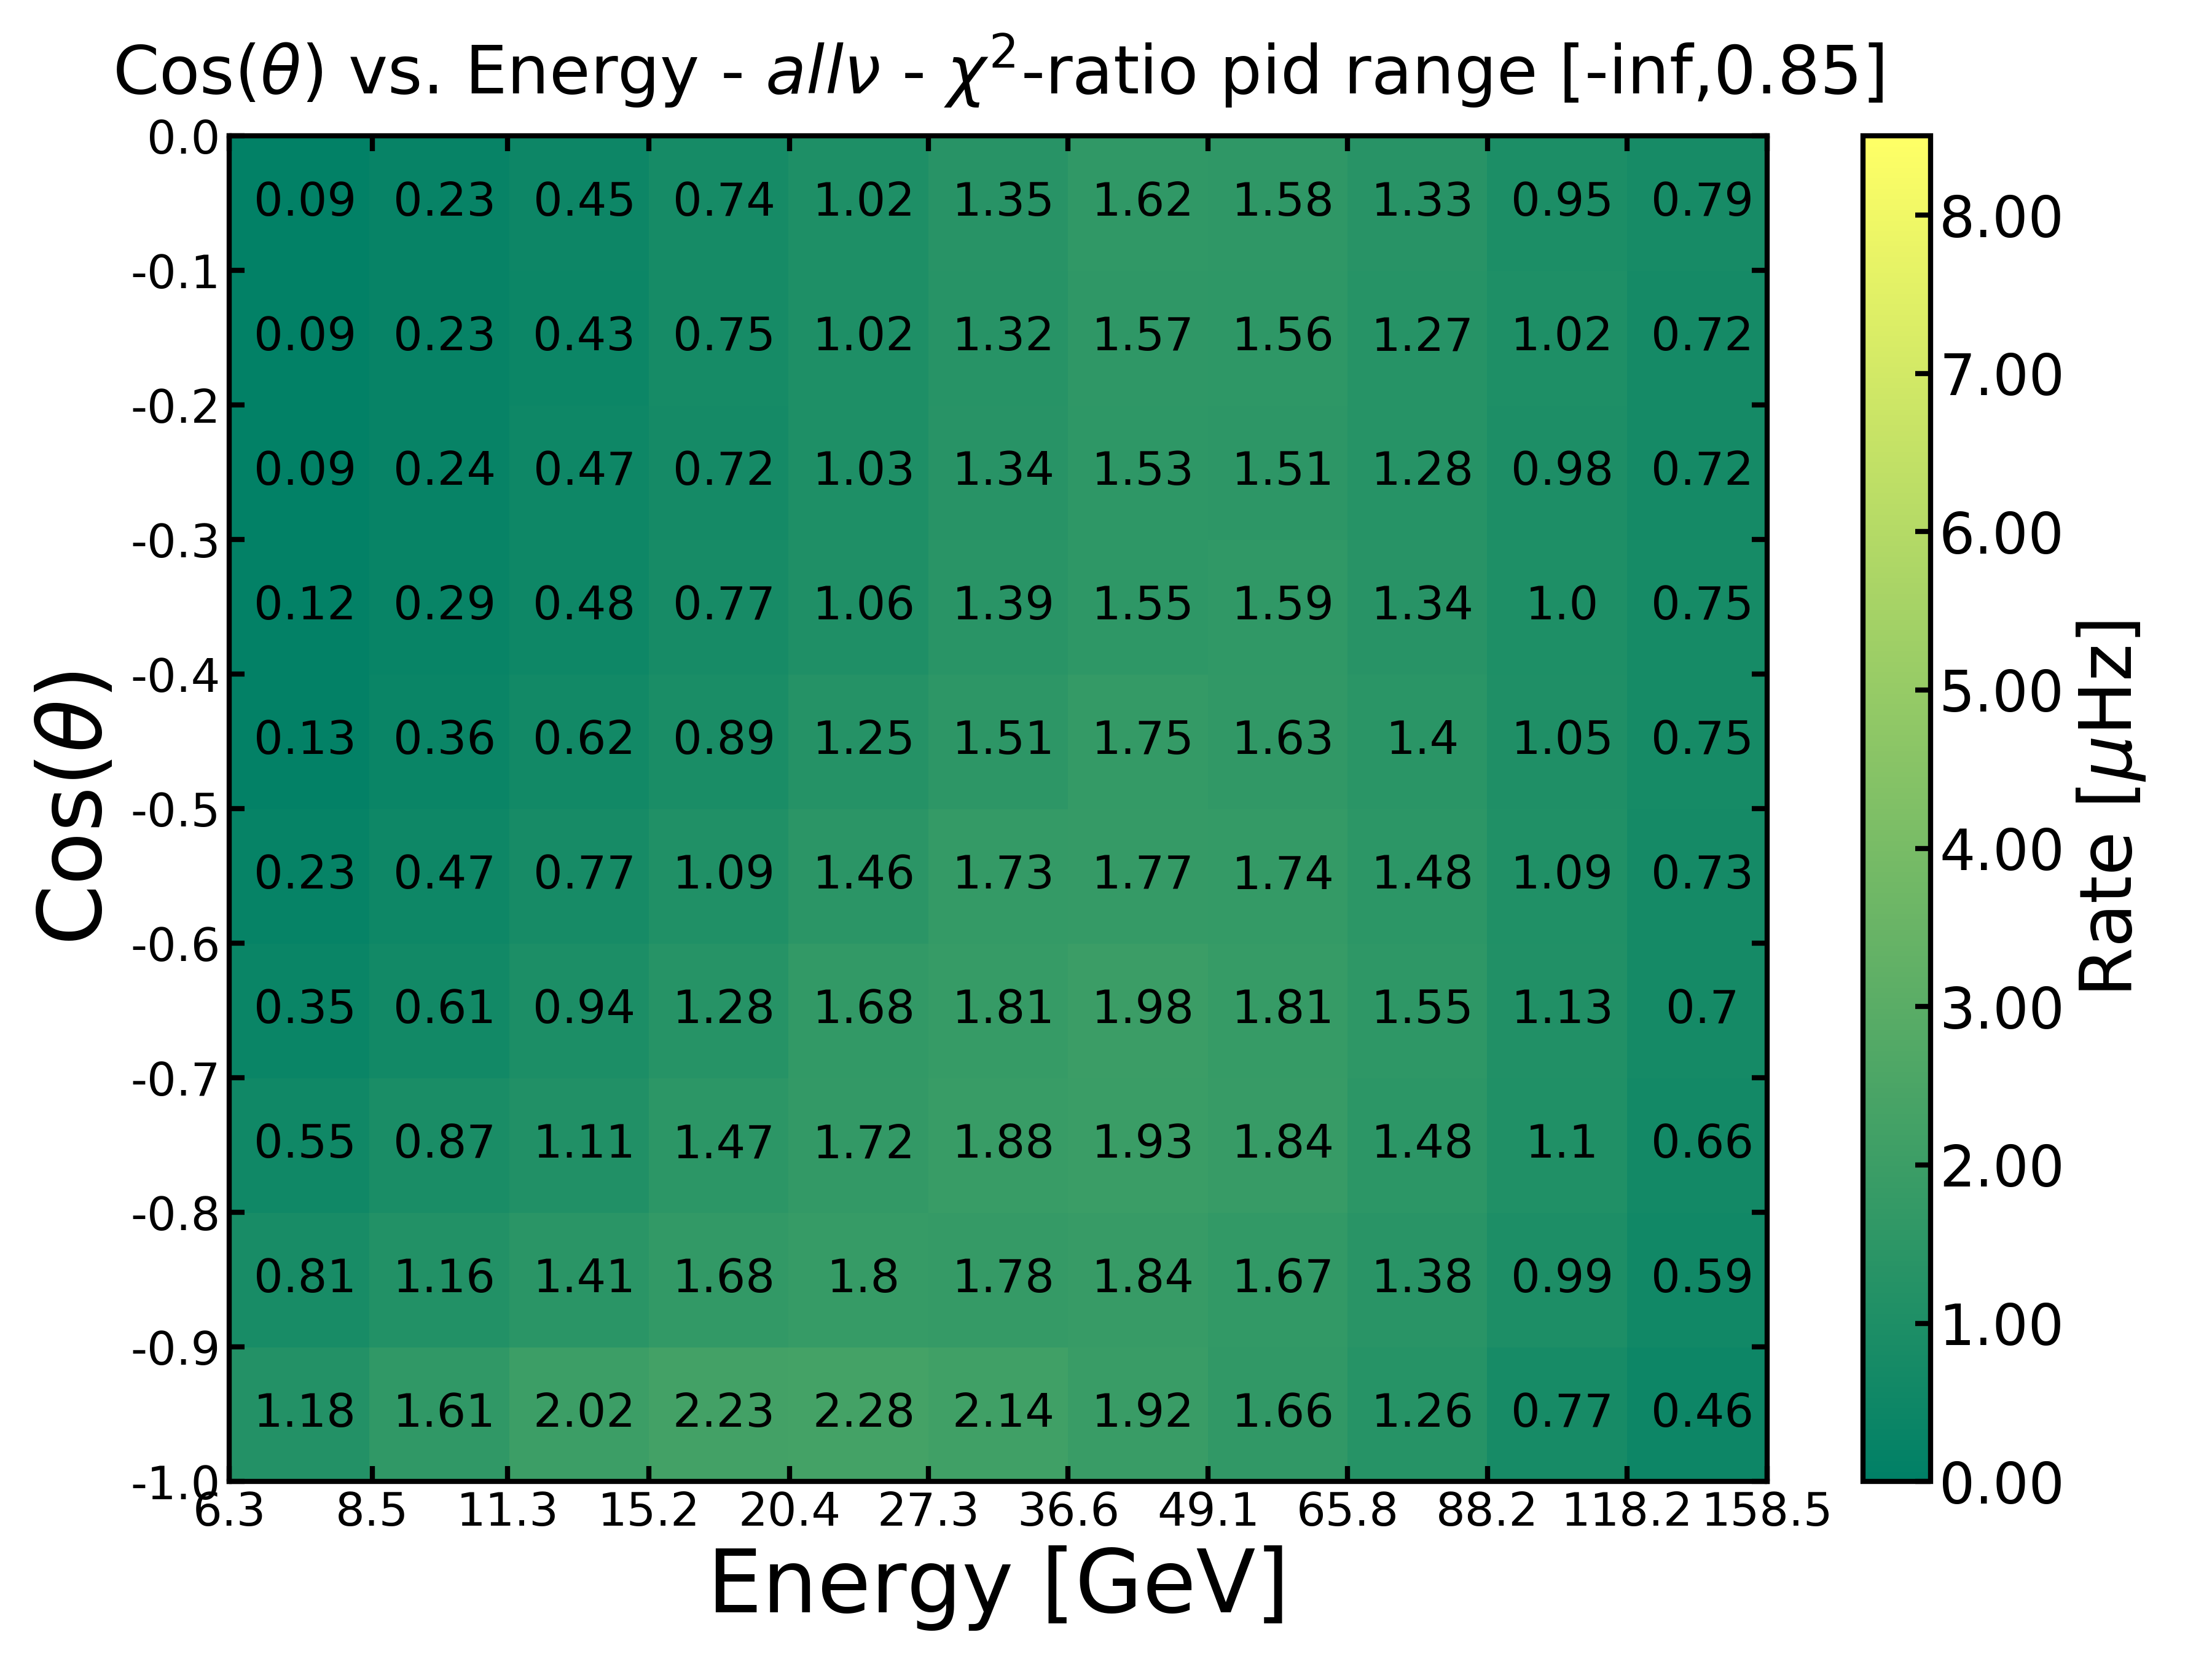
\includegraphics[width=0.49\linewidth]{figures/santa_cut_085_allnu_0_unoscillated_vmax.png}
    \caption[Expected unoscillated event rates for two-bin case with $\chi^2\textrm{-ratio}$ PID]{Expected unoscillated event rates for two-bin case with $\chi^2\textrm{-ratio}$ PID.}
    \label{fig:unoscillated_histrograms_santa_2bin}
\end{figure}

\begin{figure}[h]
    \centering
    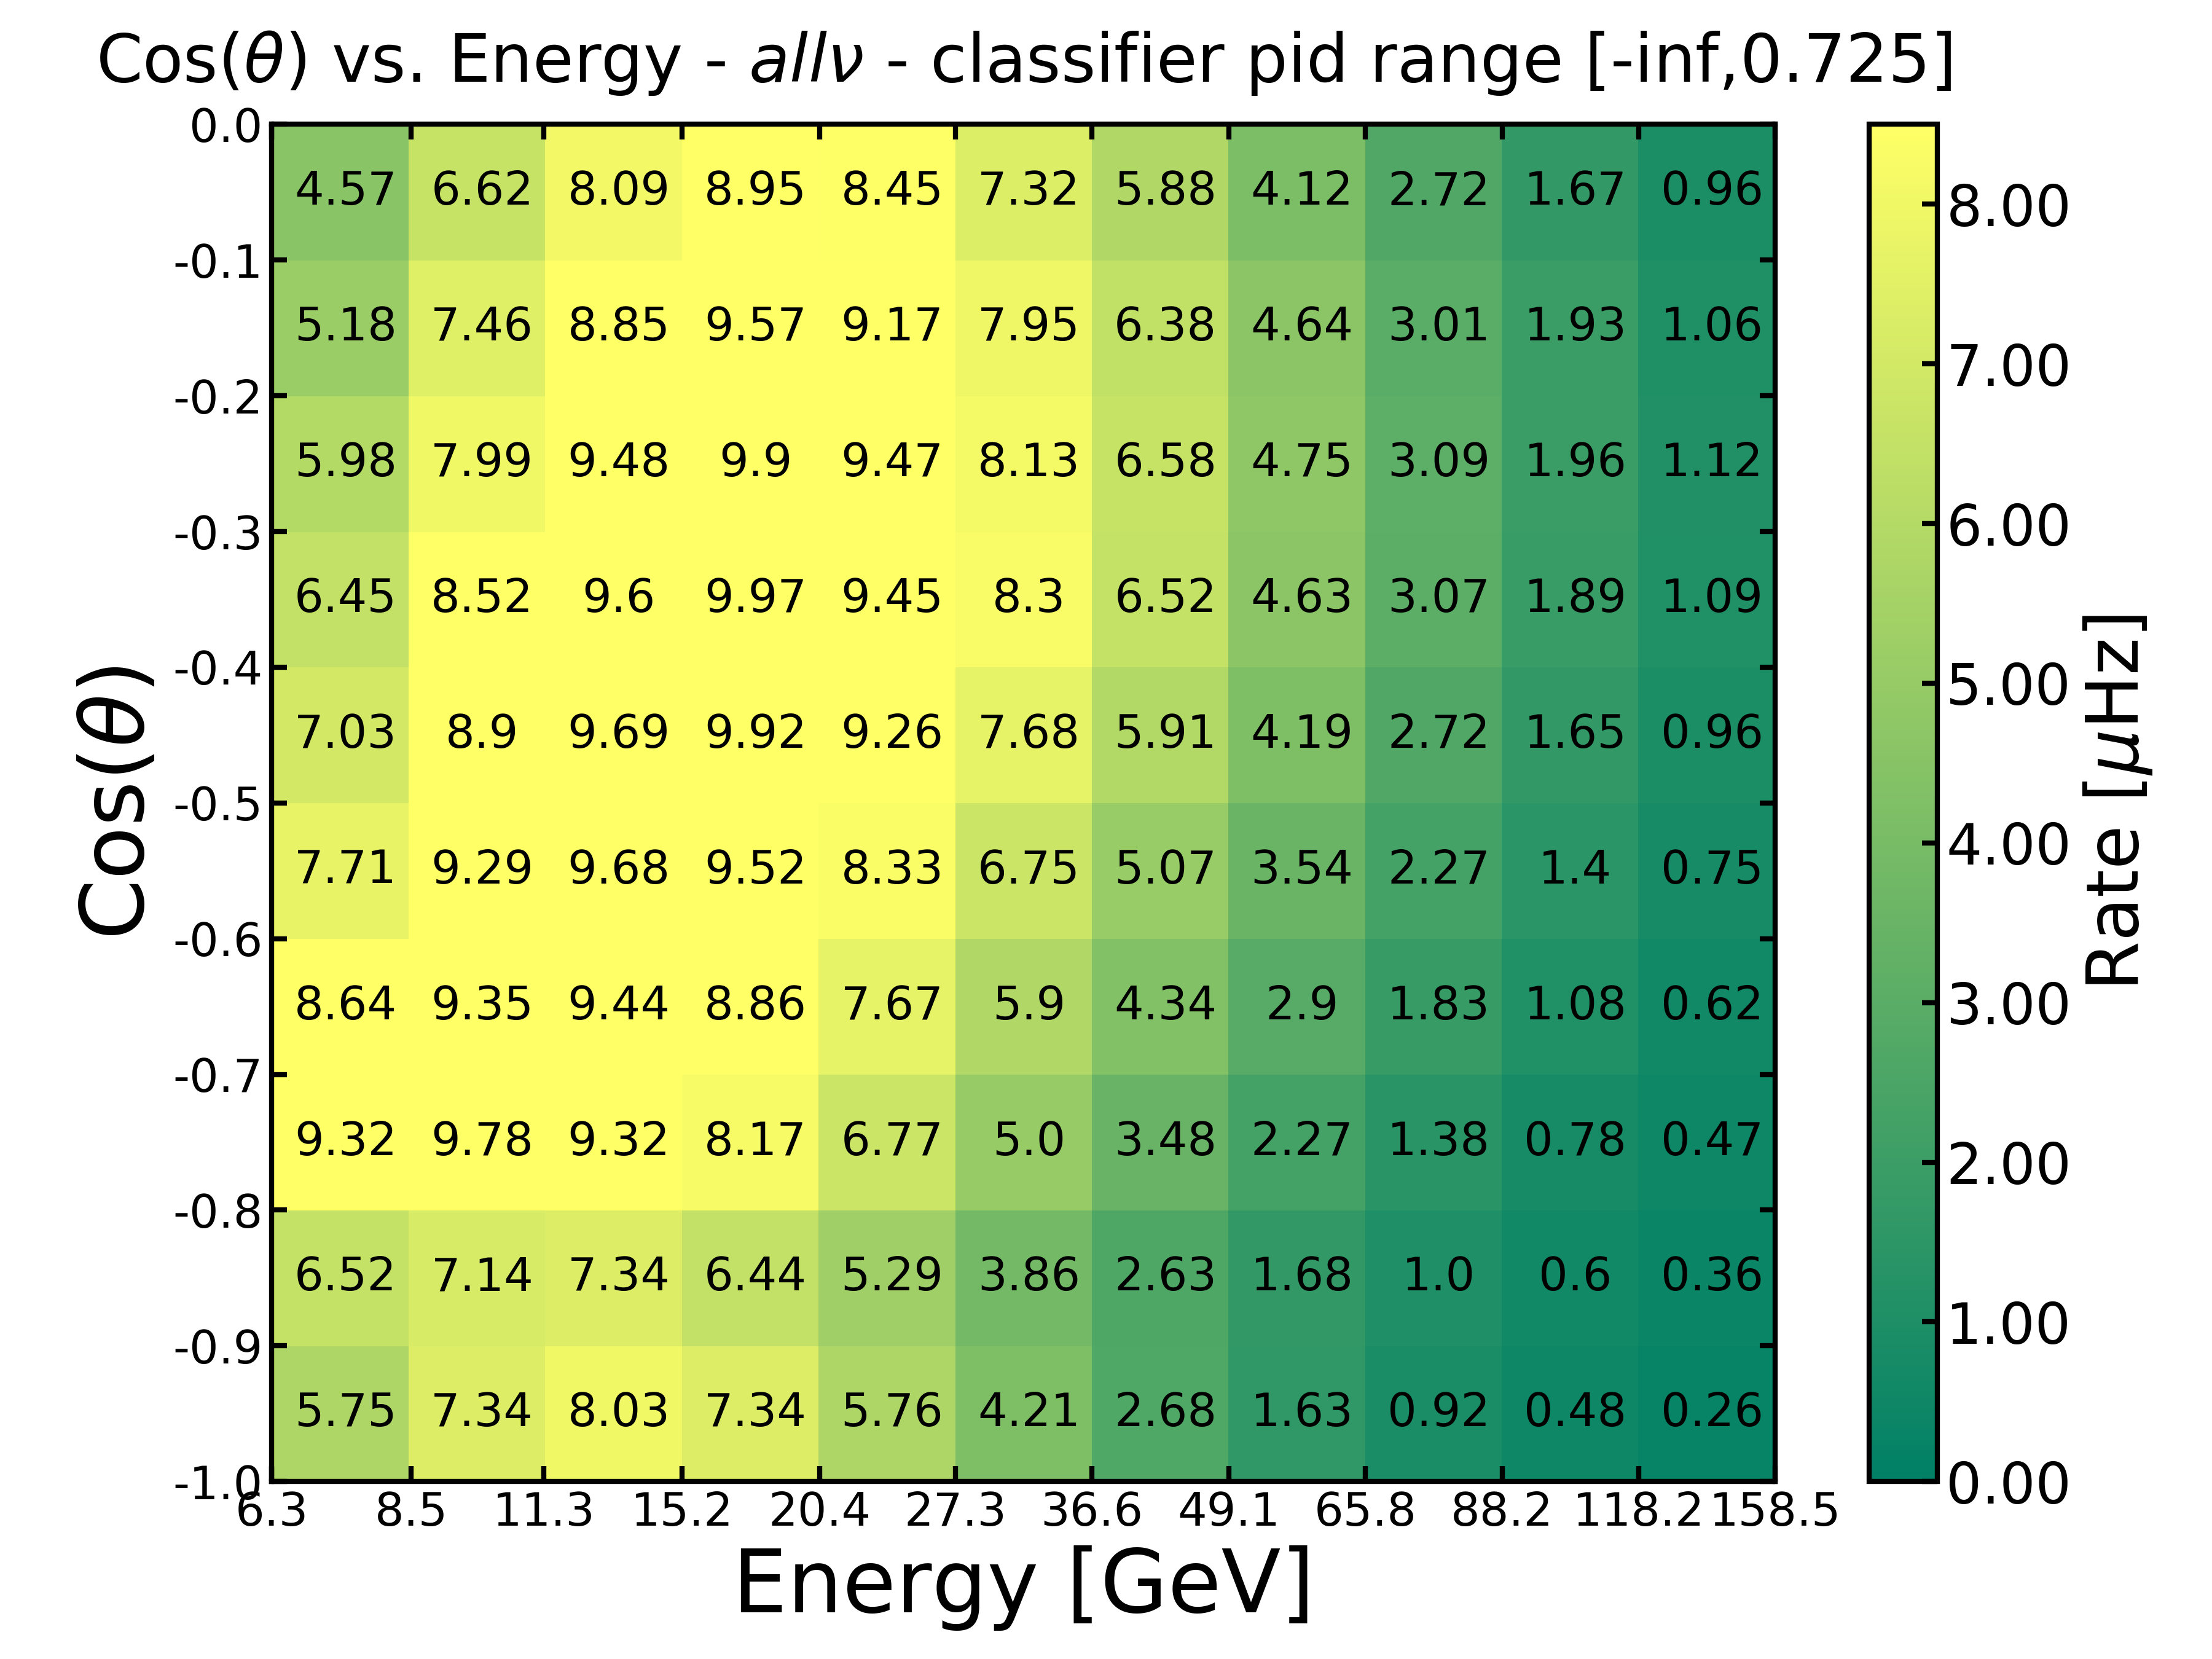
\includegraphics[width=0.49\linewidth]{figures/two_bin_cut_0725_allnu_0_unoscillated_vmax.png}
    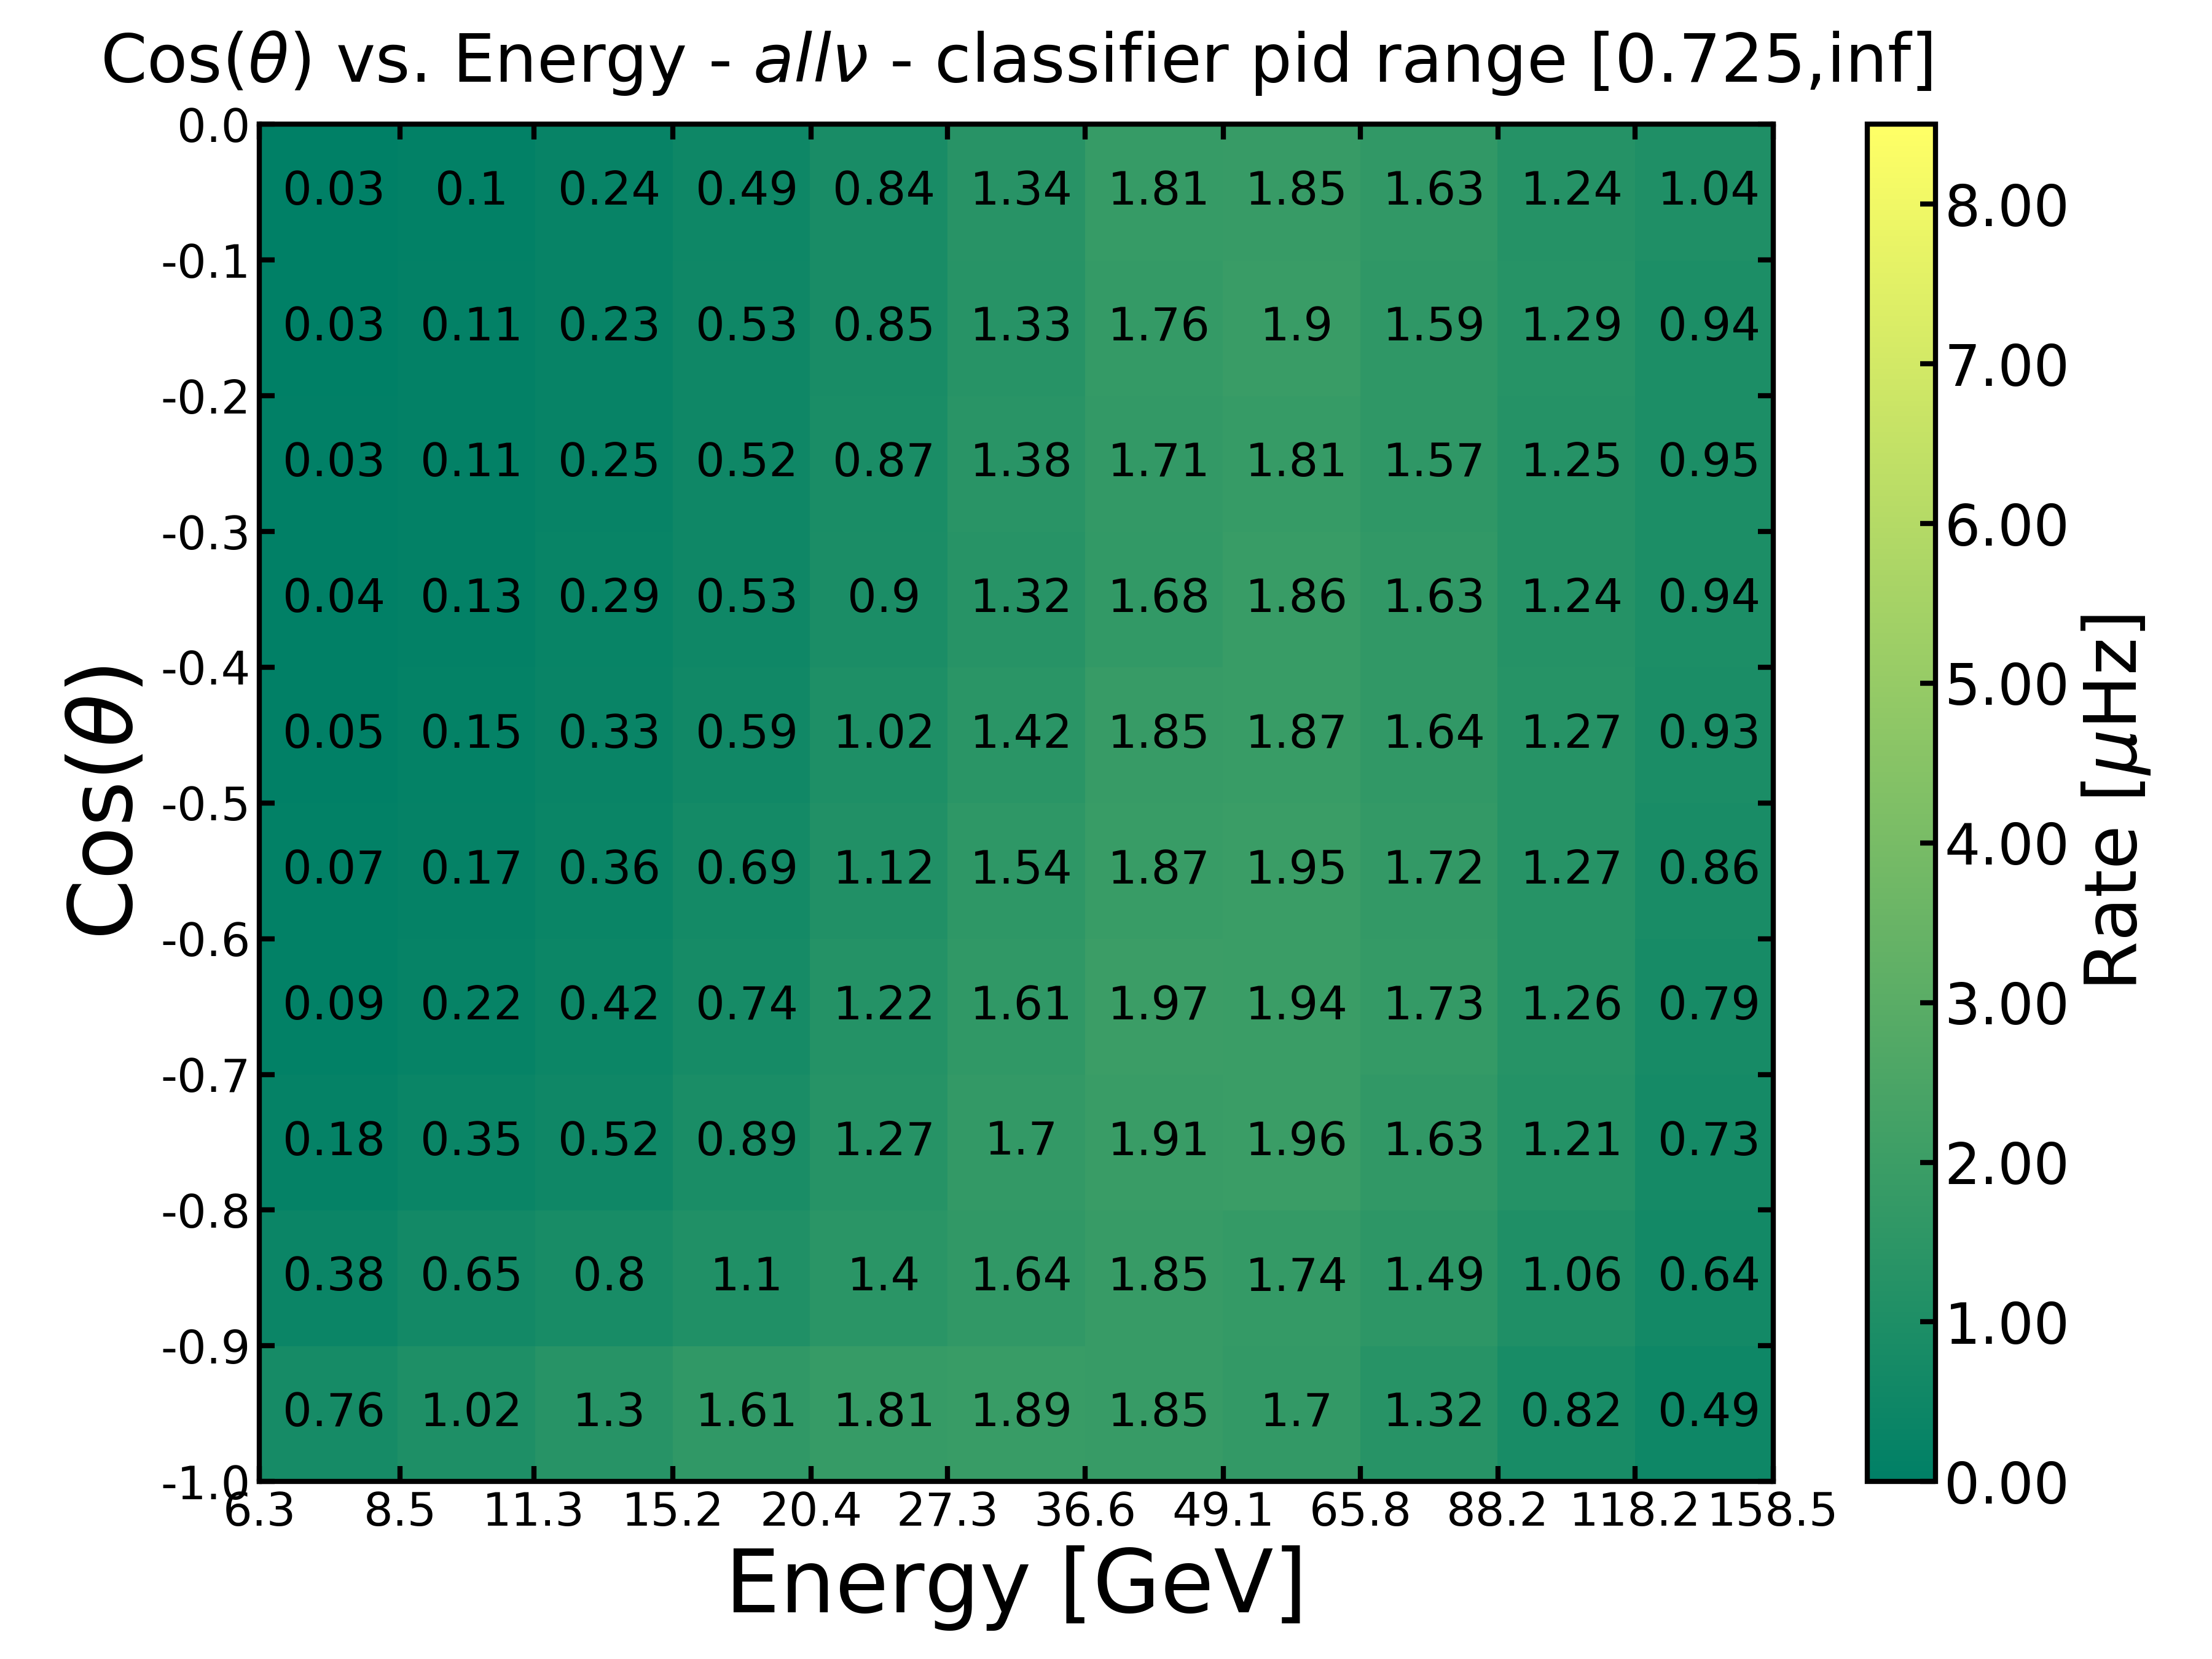
\includegraphics[width=0.49\linewidth]{figures/two_bin_cut_0725_allnu_1_unoscillated_vmax.png}
    \caption[Expected unoscillated event rates for two-bin case with classifier PID]{Expected unoscillated event rates for two-bin case with classifier PID.}
    \label{fig:unoscillated_histrograms_classifier_2bin}
\end{figure}

\begin{figure}[h]
    \centering
    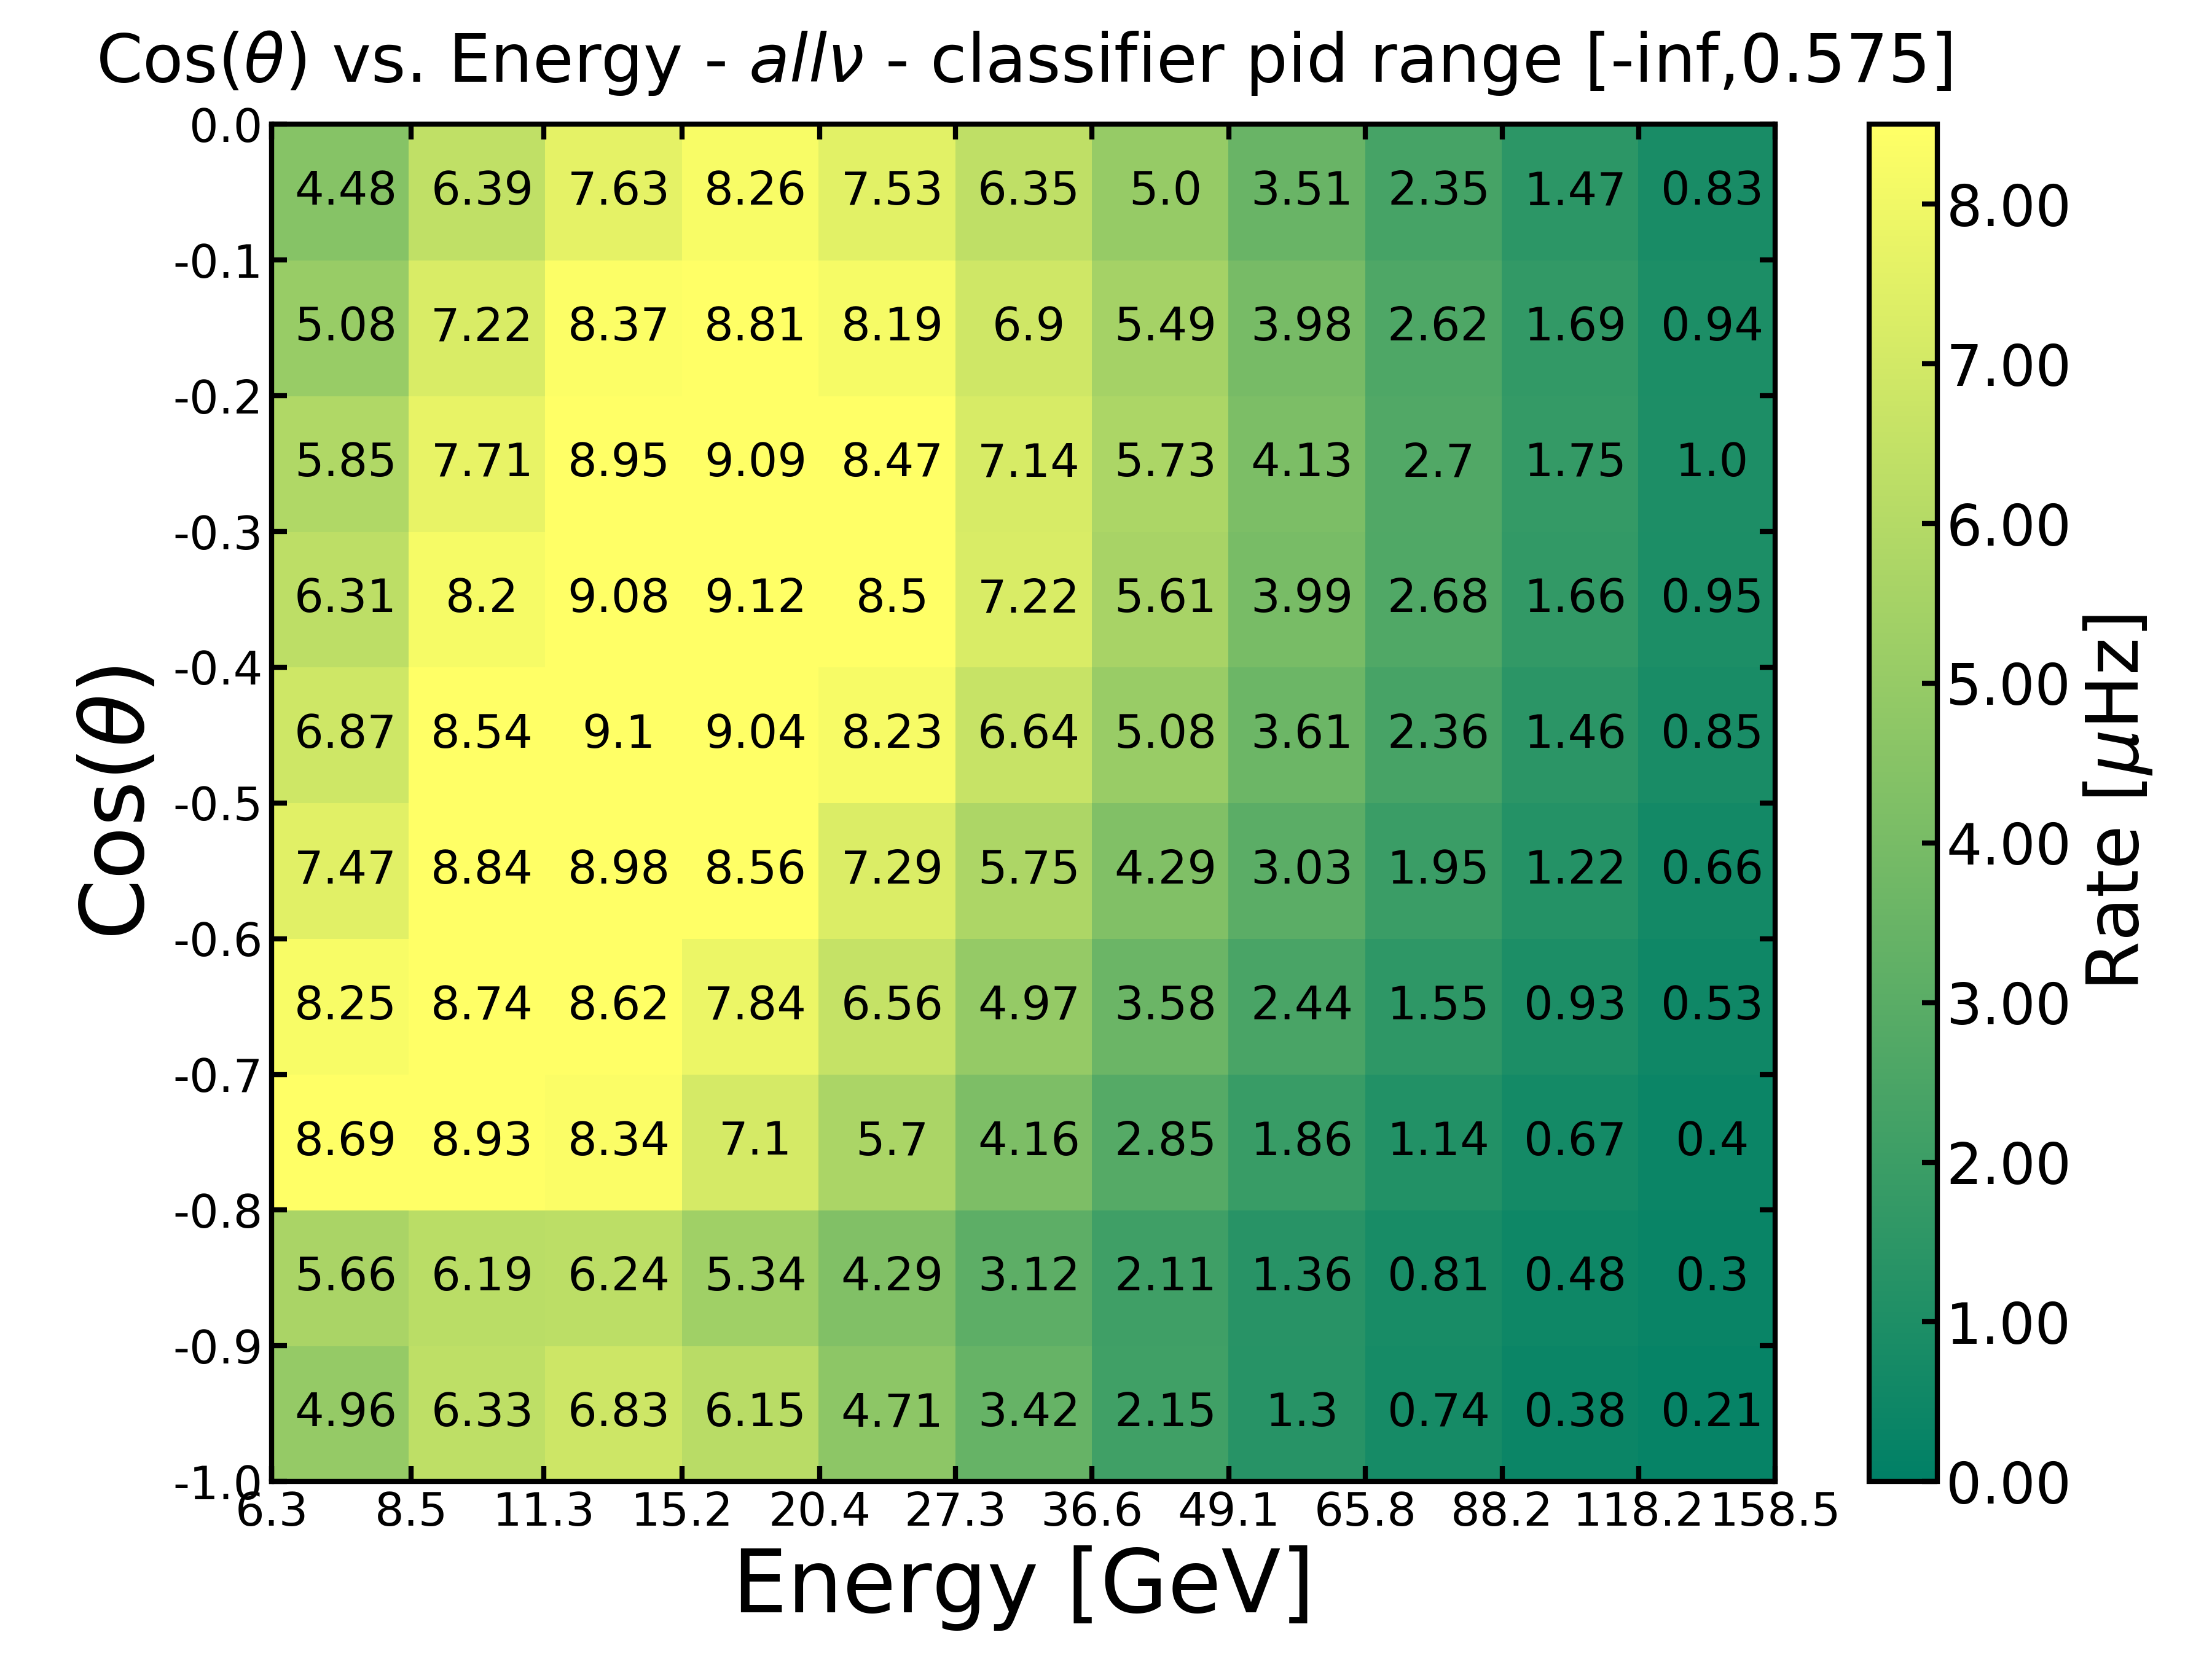
\includegraphics[width=0.49\linewidth]{figures/three_bin_cut_0575_0825_allnu_0_unoscillated_vmax.png}
    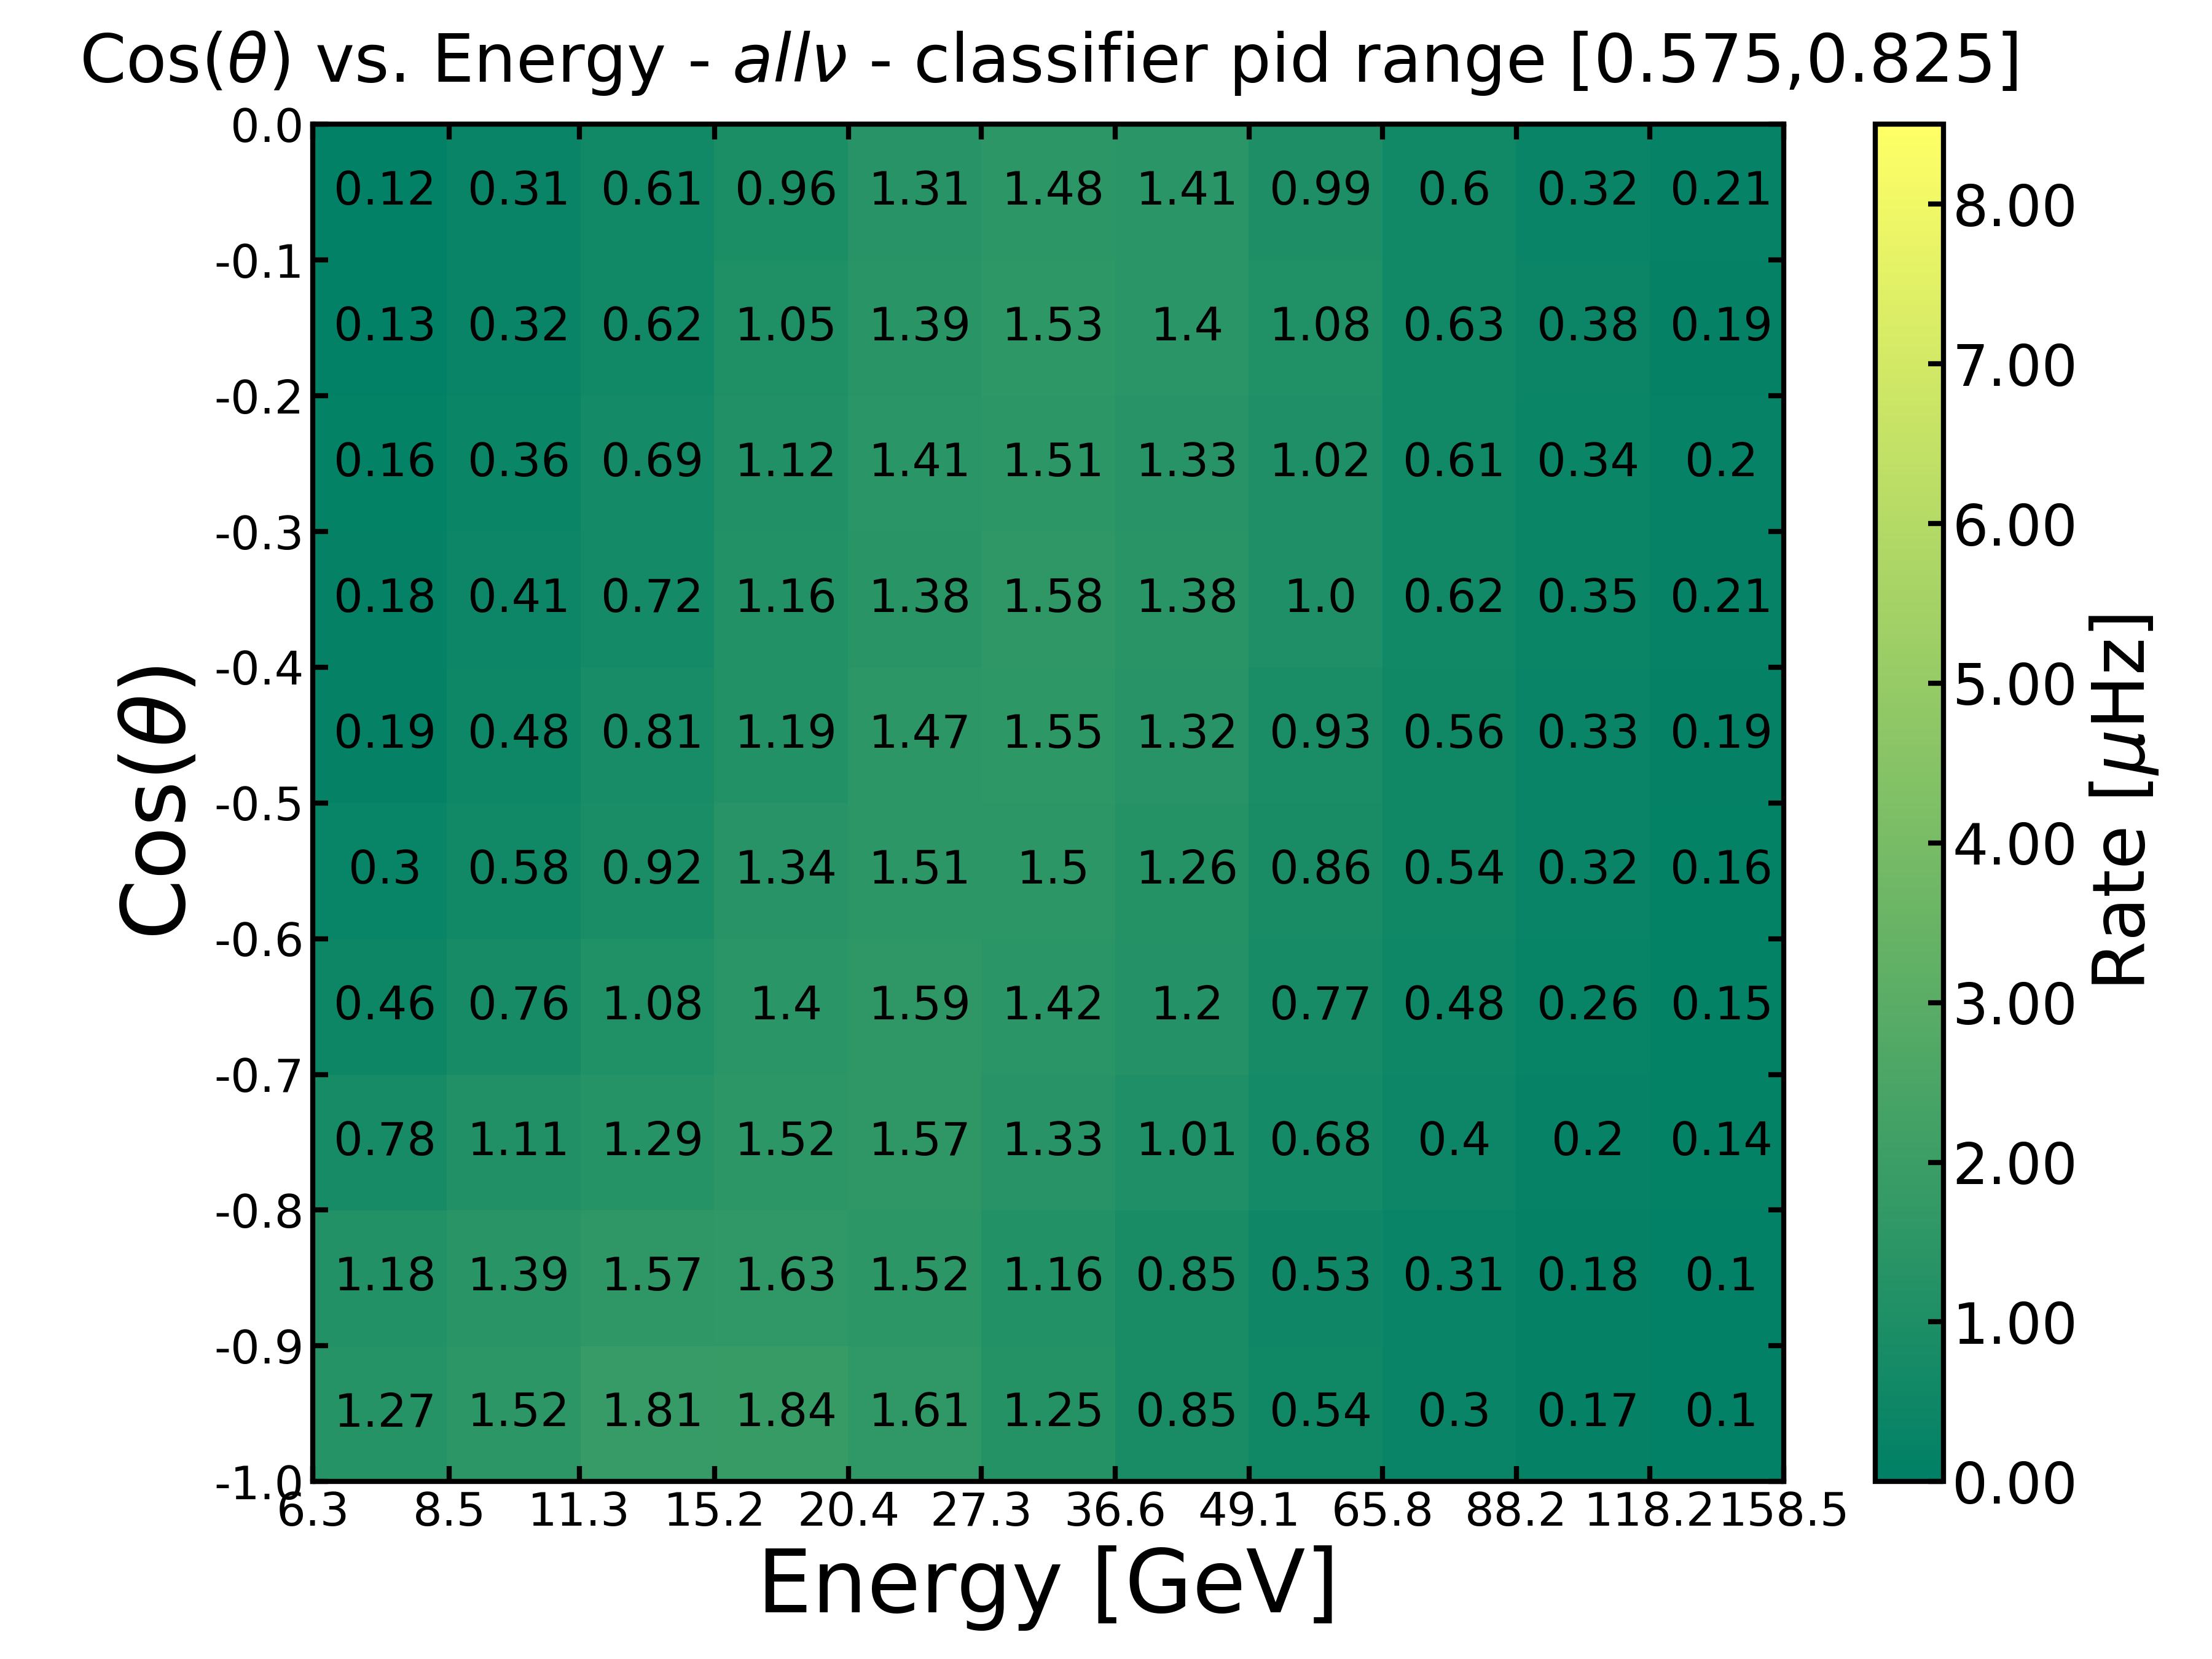
\includegraphics[width=0.49\linewidth]{figures/three_bin_cut_0575_0825_allnu_1_unoscillated_vmax.png}
    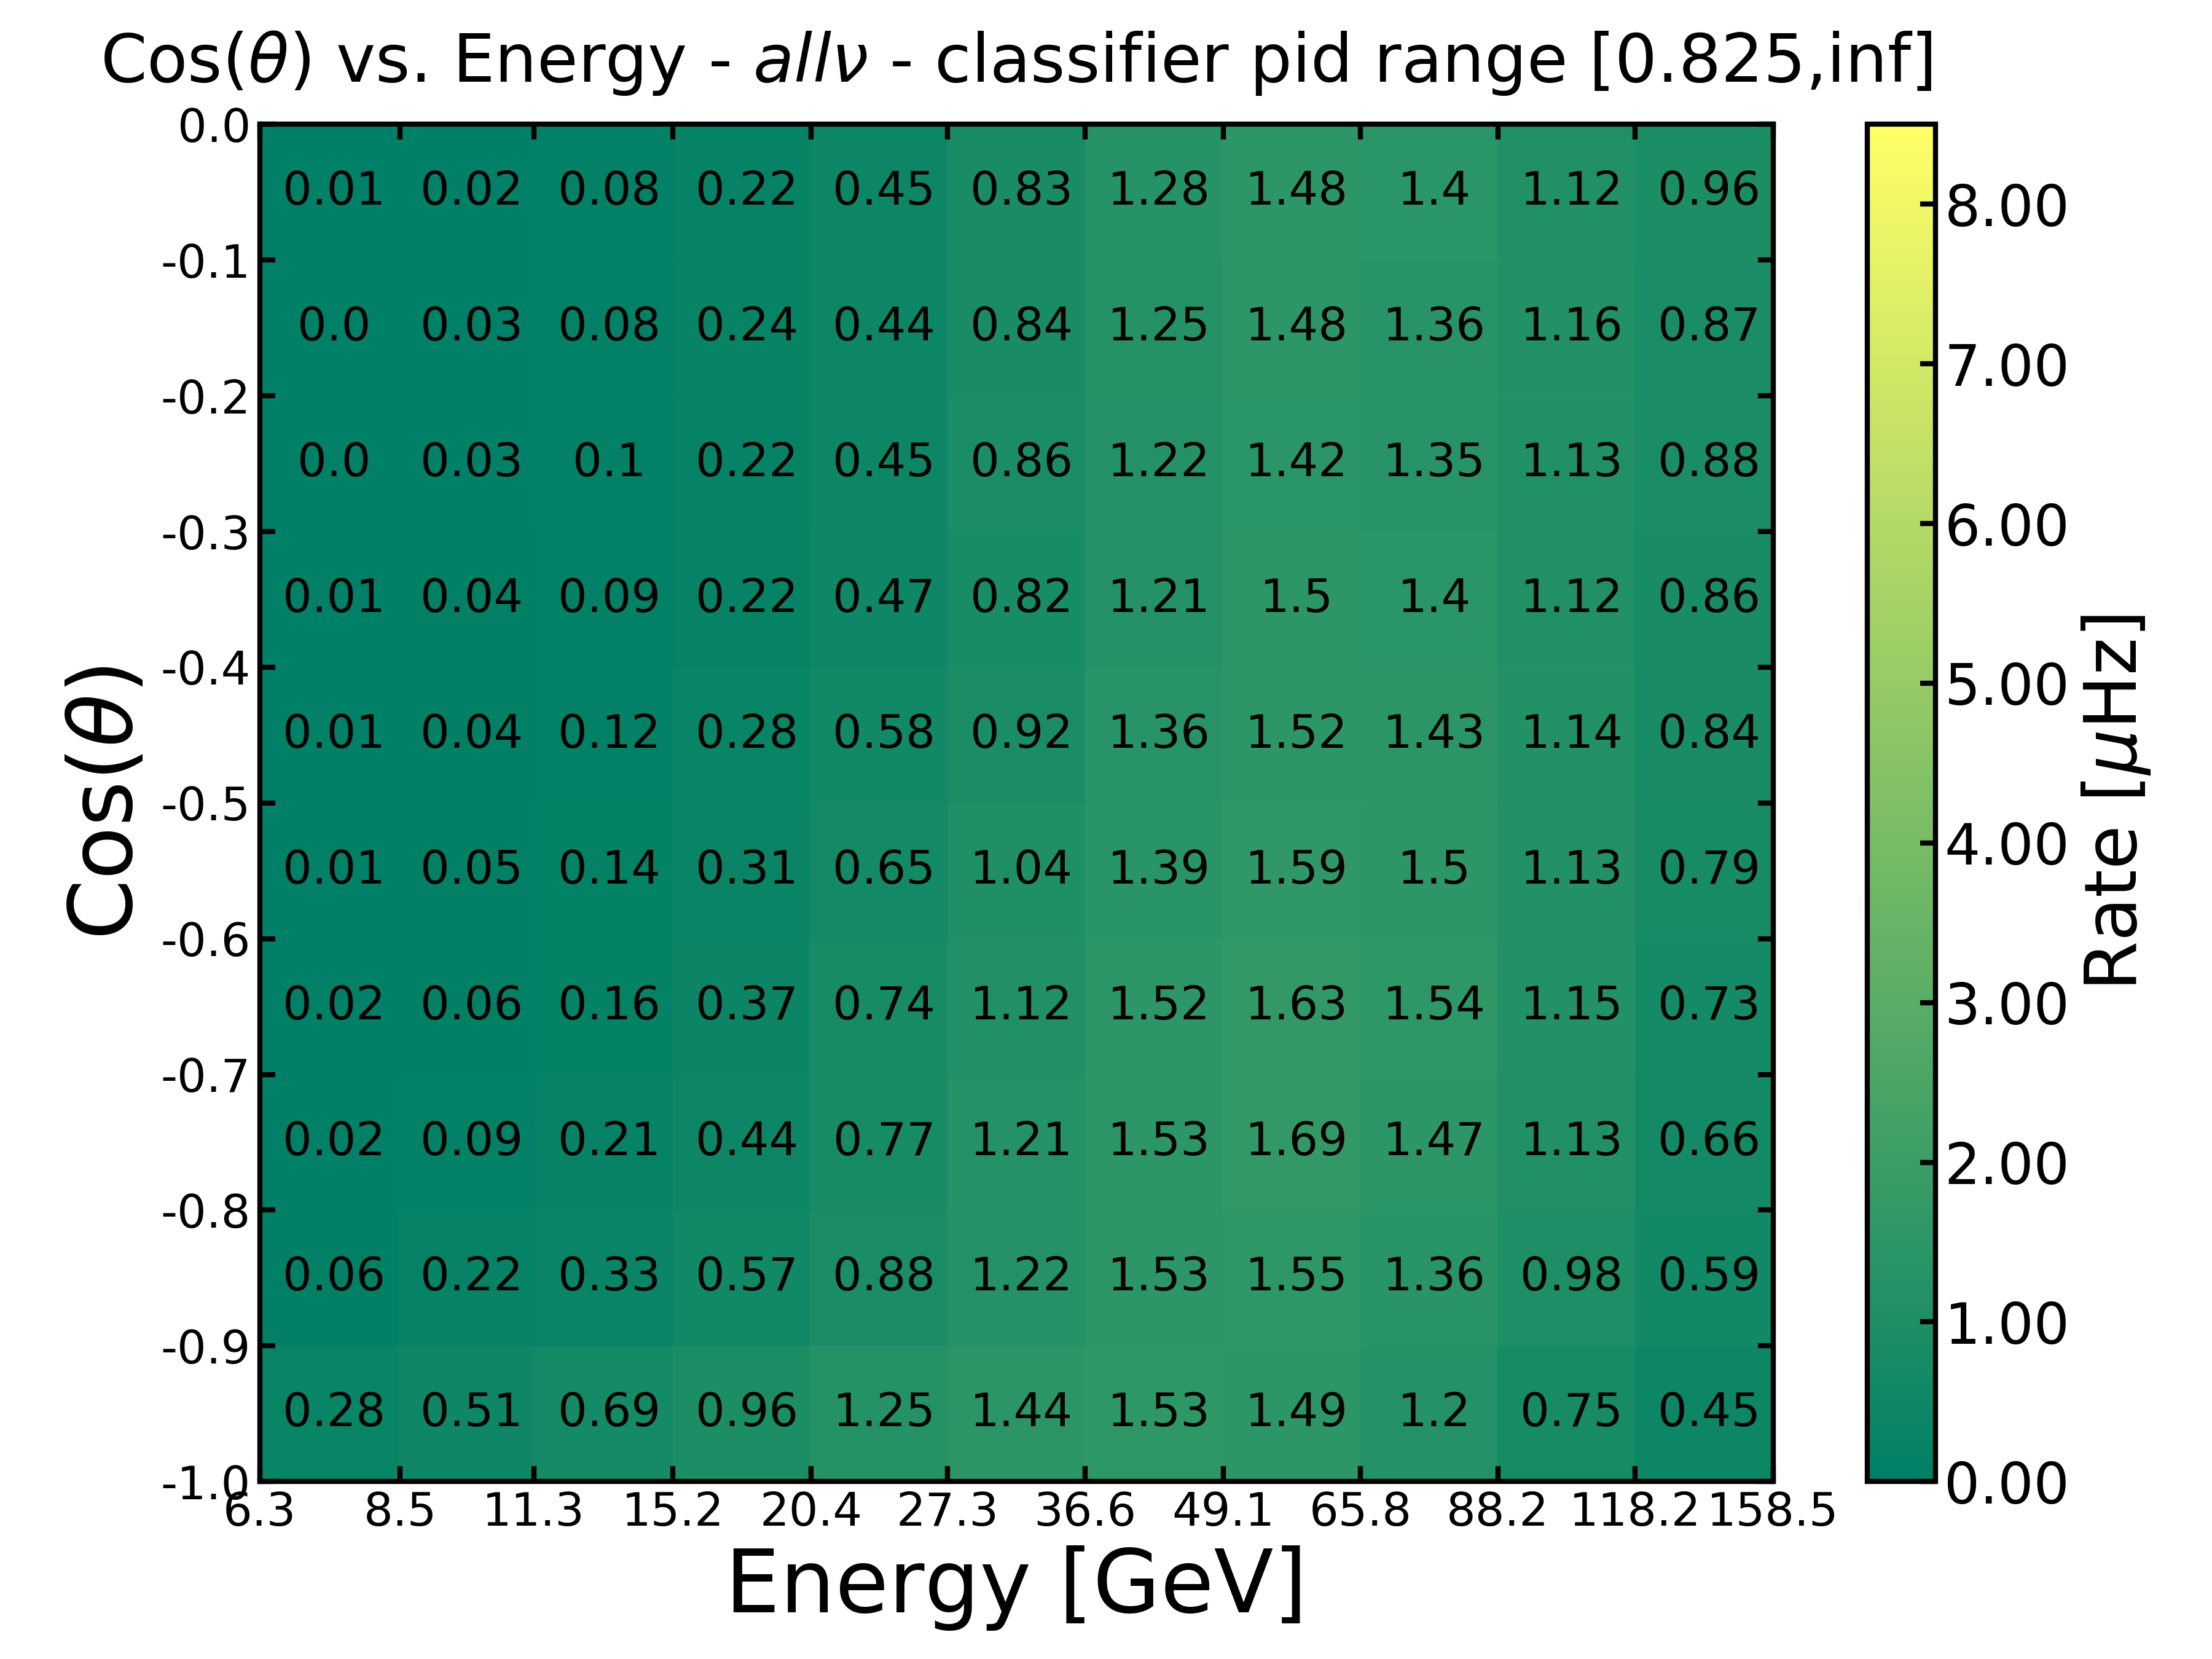
\includegraphics[width=0.49\linewidth]{figures/three_bin_cut_0575_0825_allnu_2_unoscillated_vmax.png}
    \caption[Expected unoscillated event rates for three-bin case with classifier PID]{Expected unoscillated event rates for three-bin case with classifier PID.}
    \label{fig:unoscillated_histrograms_classifier_3bin}
\end{figure}

\begin{figure}[h]
    \centering
    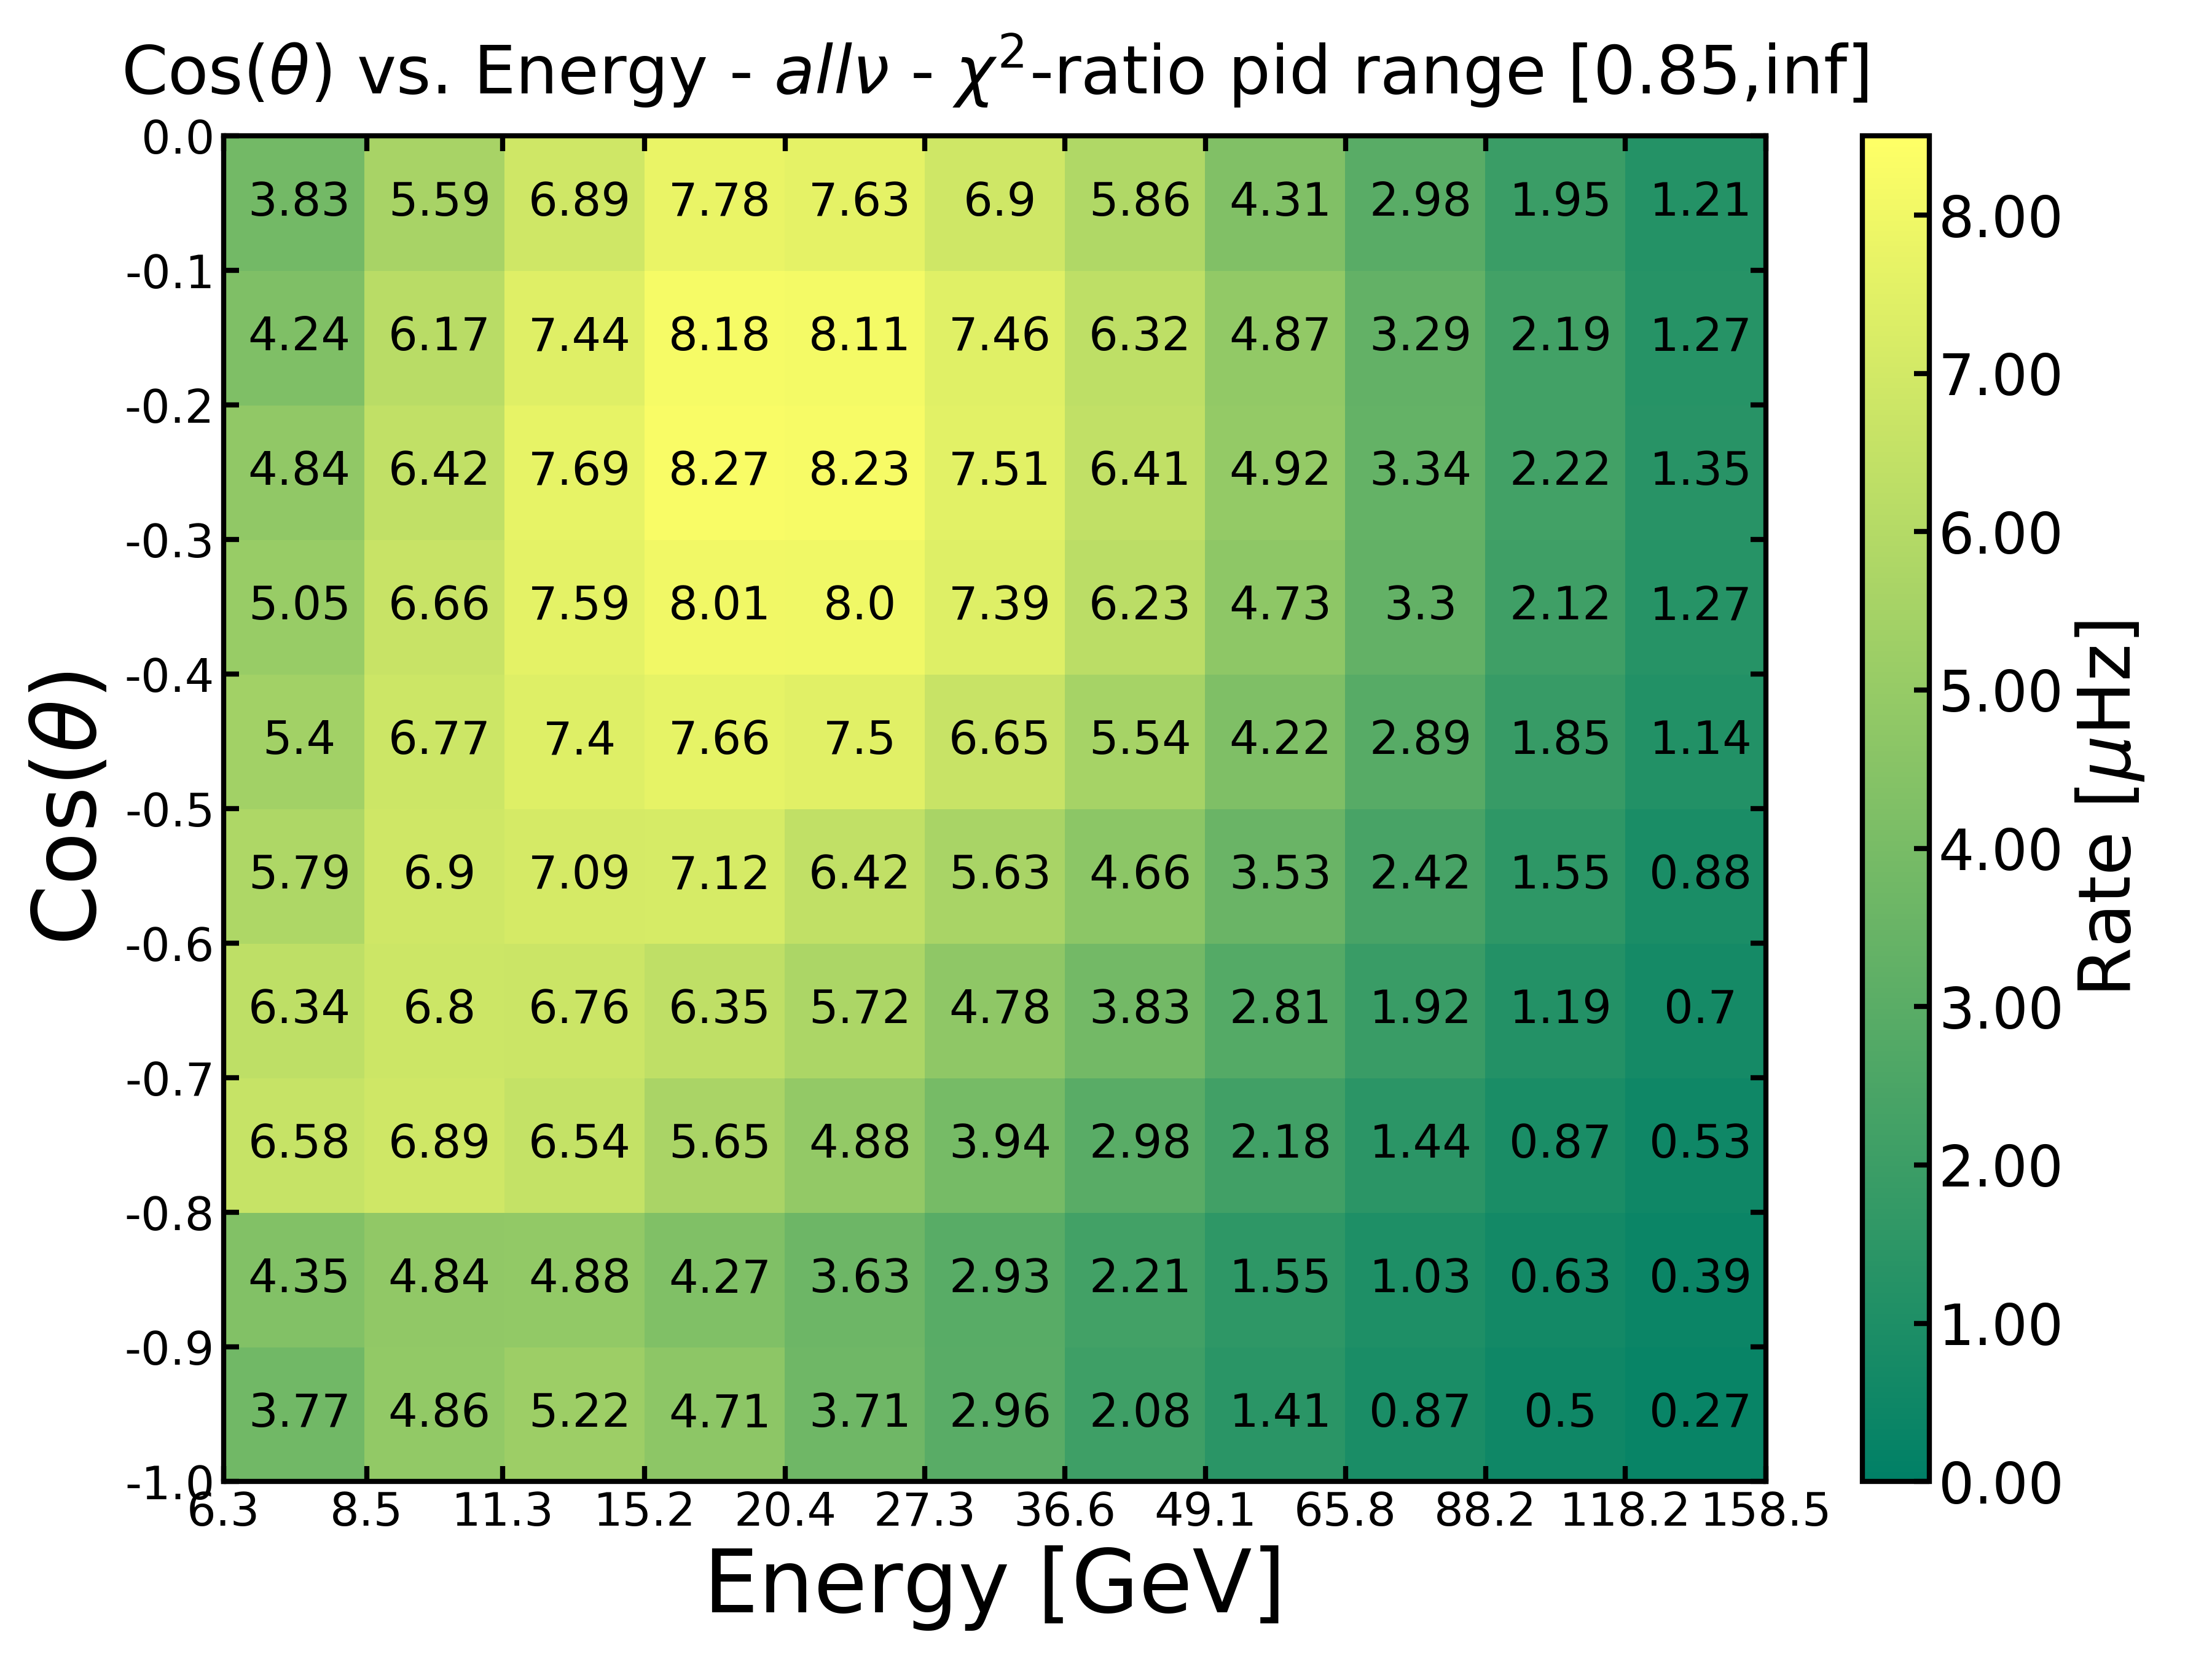
\includegraphics[width=0.49\linewidth]{figures/santa_cut_085_allnu_1_oscillated_vmax.png}
    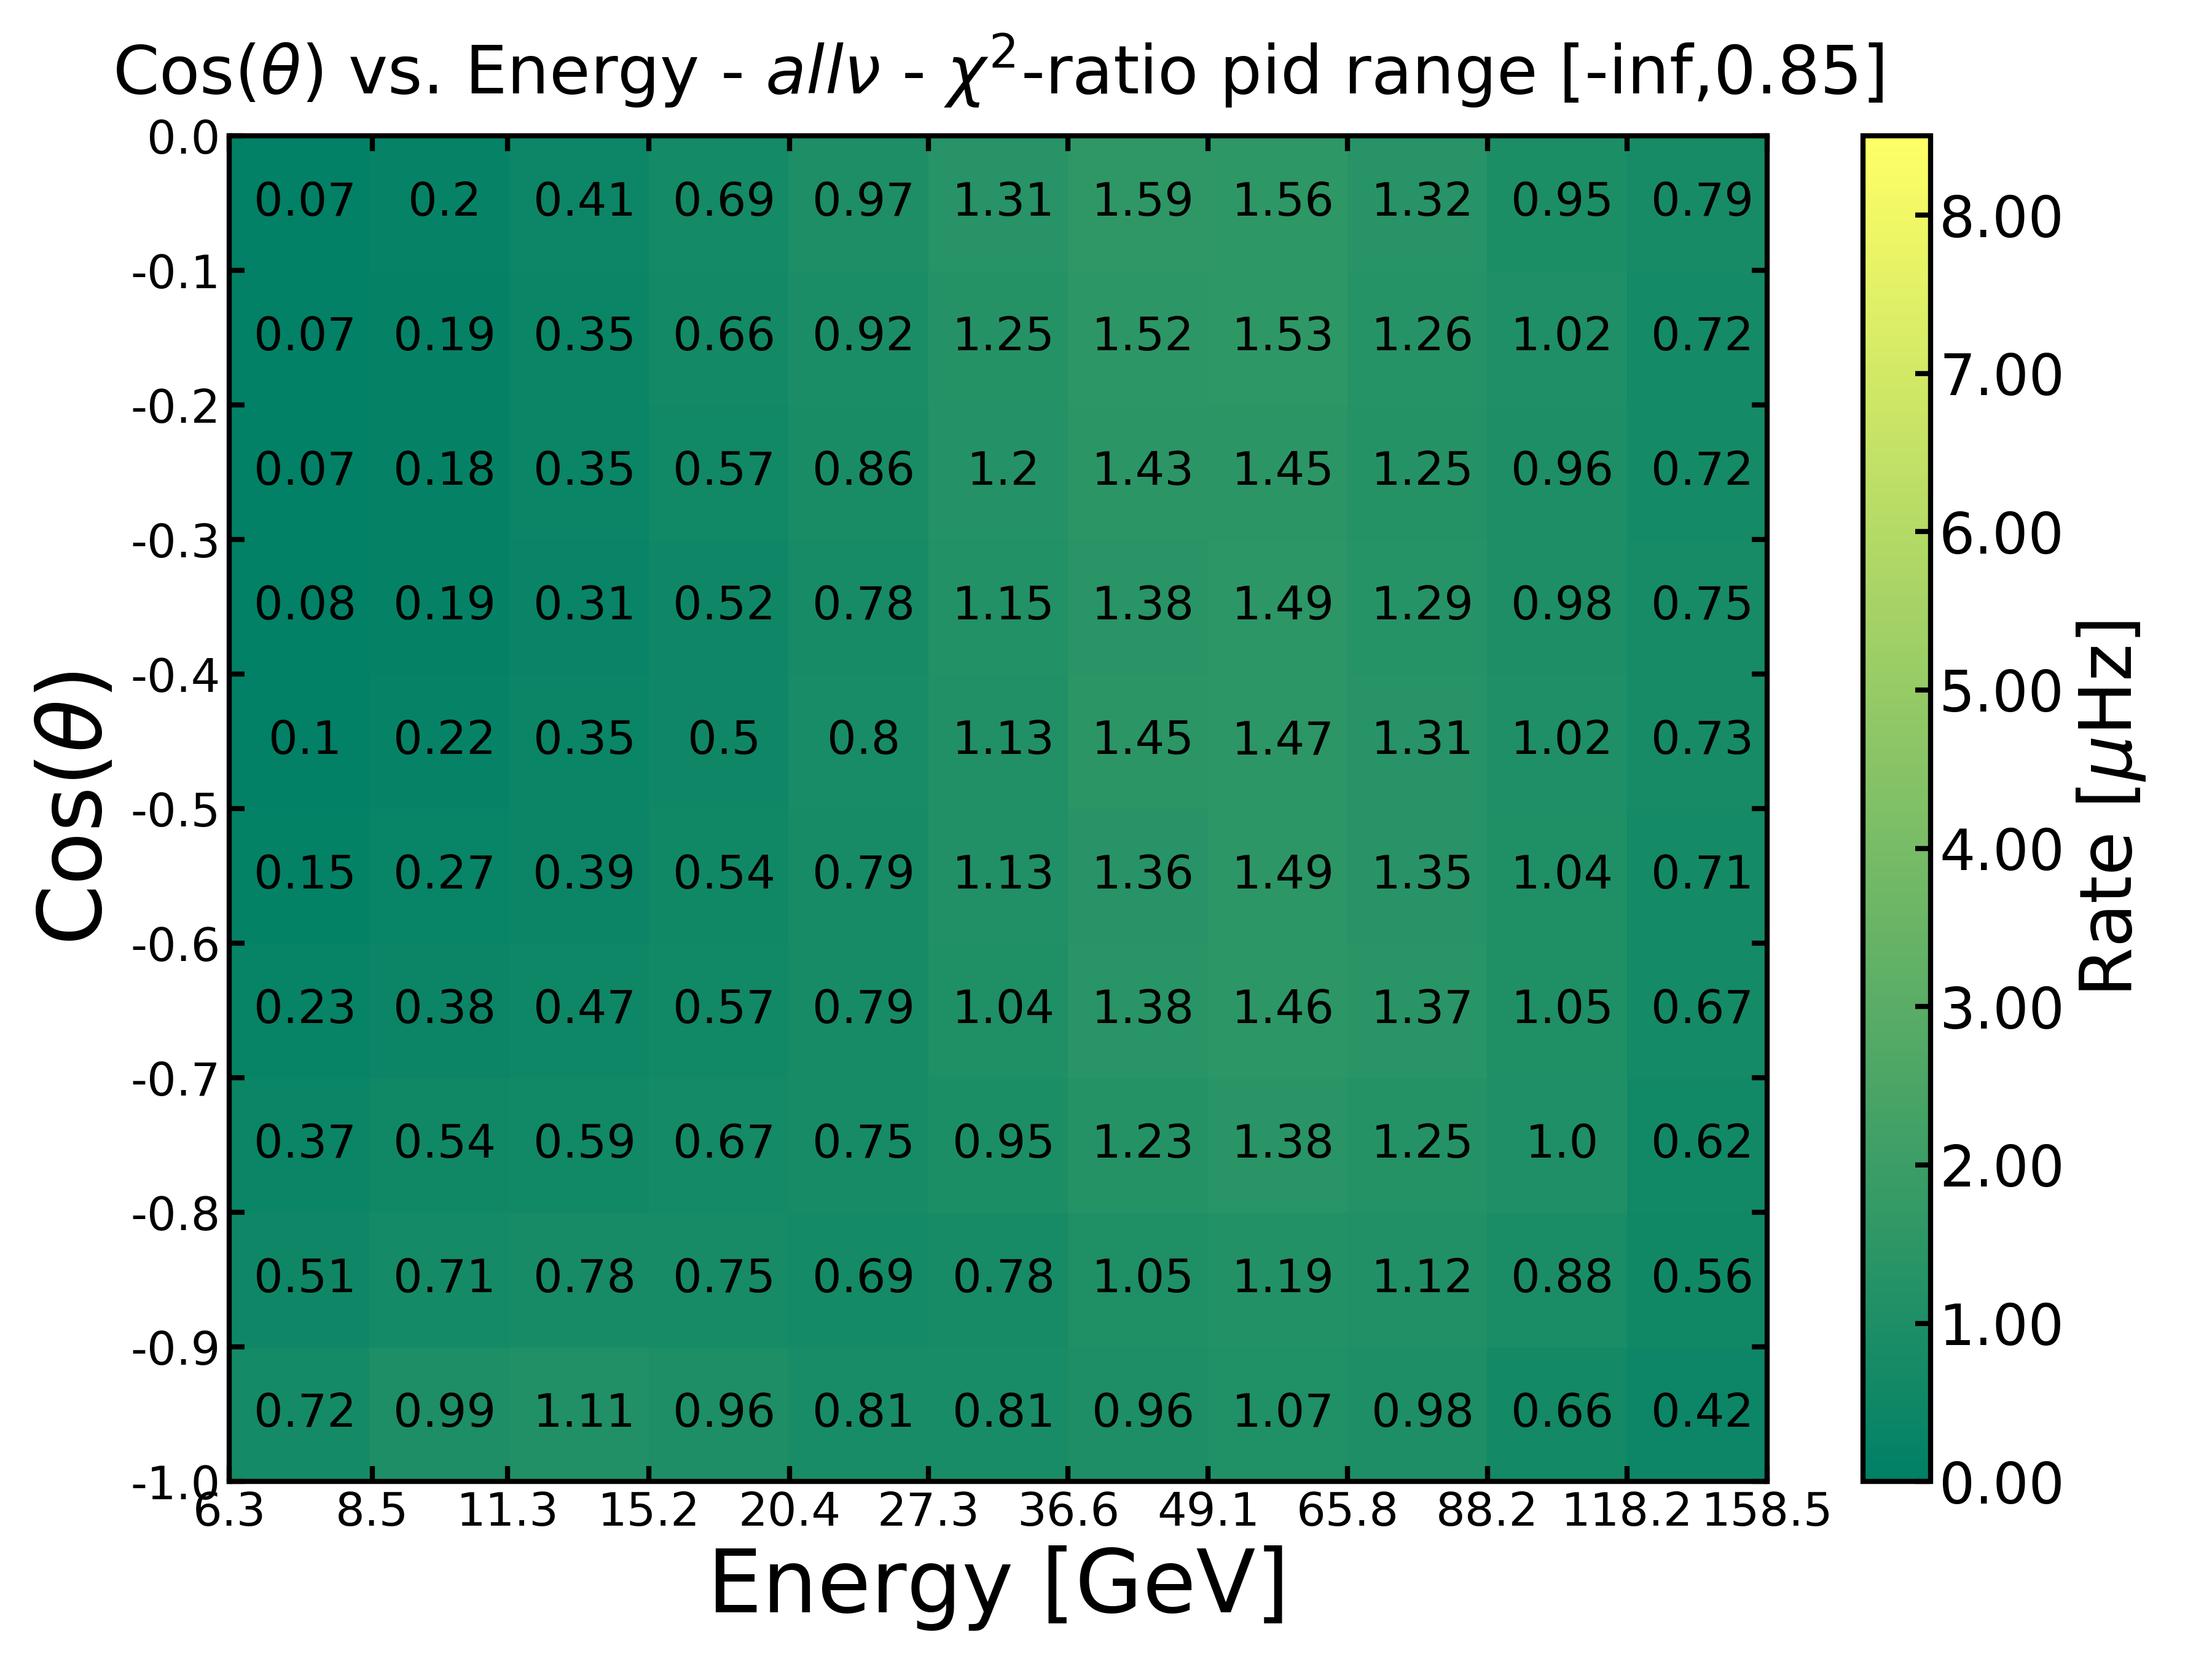
\includegraphics[width=0.49\linewidth]{figures/santa_cut_085_allnu_0_oscillated_vmax.png}
    \caption[Expected oscillated event rates for two-bin case with $\chi^2\textrm{-ratio}$ PID]{Expected oscillated event rates for two-bin case with $\chi^2\textrm{-ratio}$ PID.}
    \label{fig:oscillated_histrograms_santa_2bin}
\end{figure}

\begin{figure}[h]
    \centering
    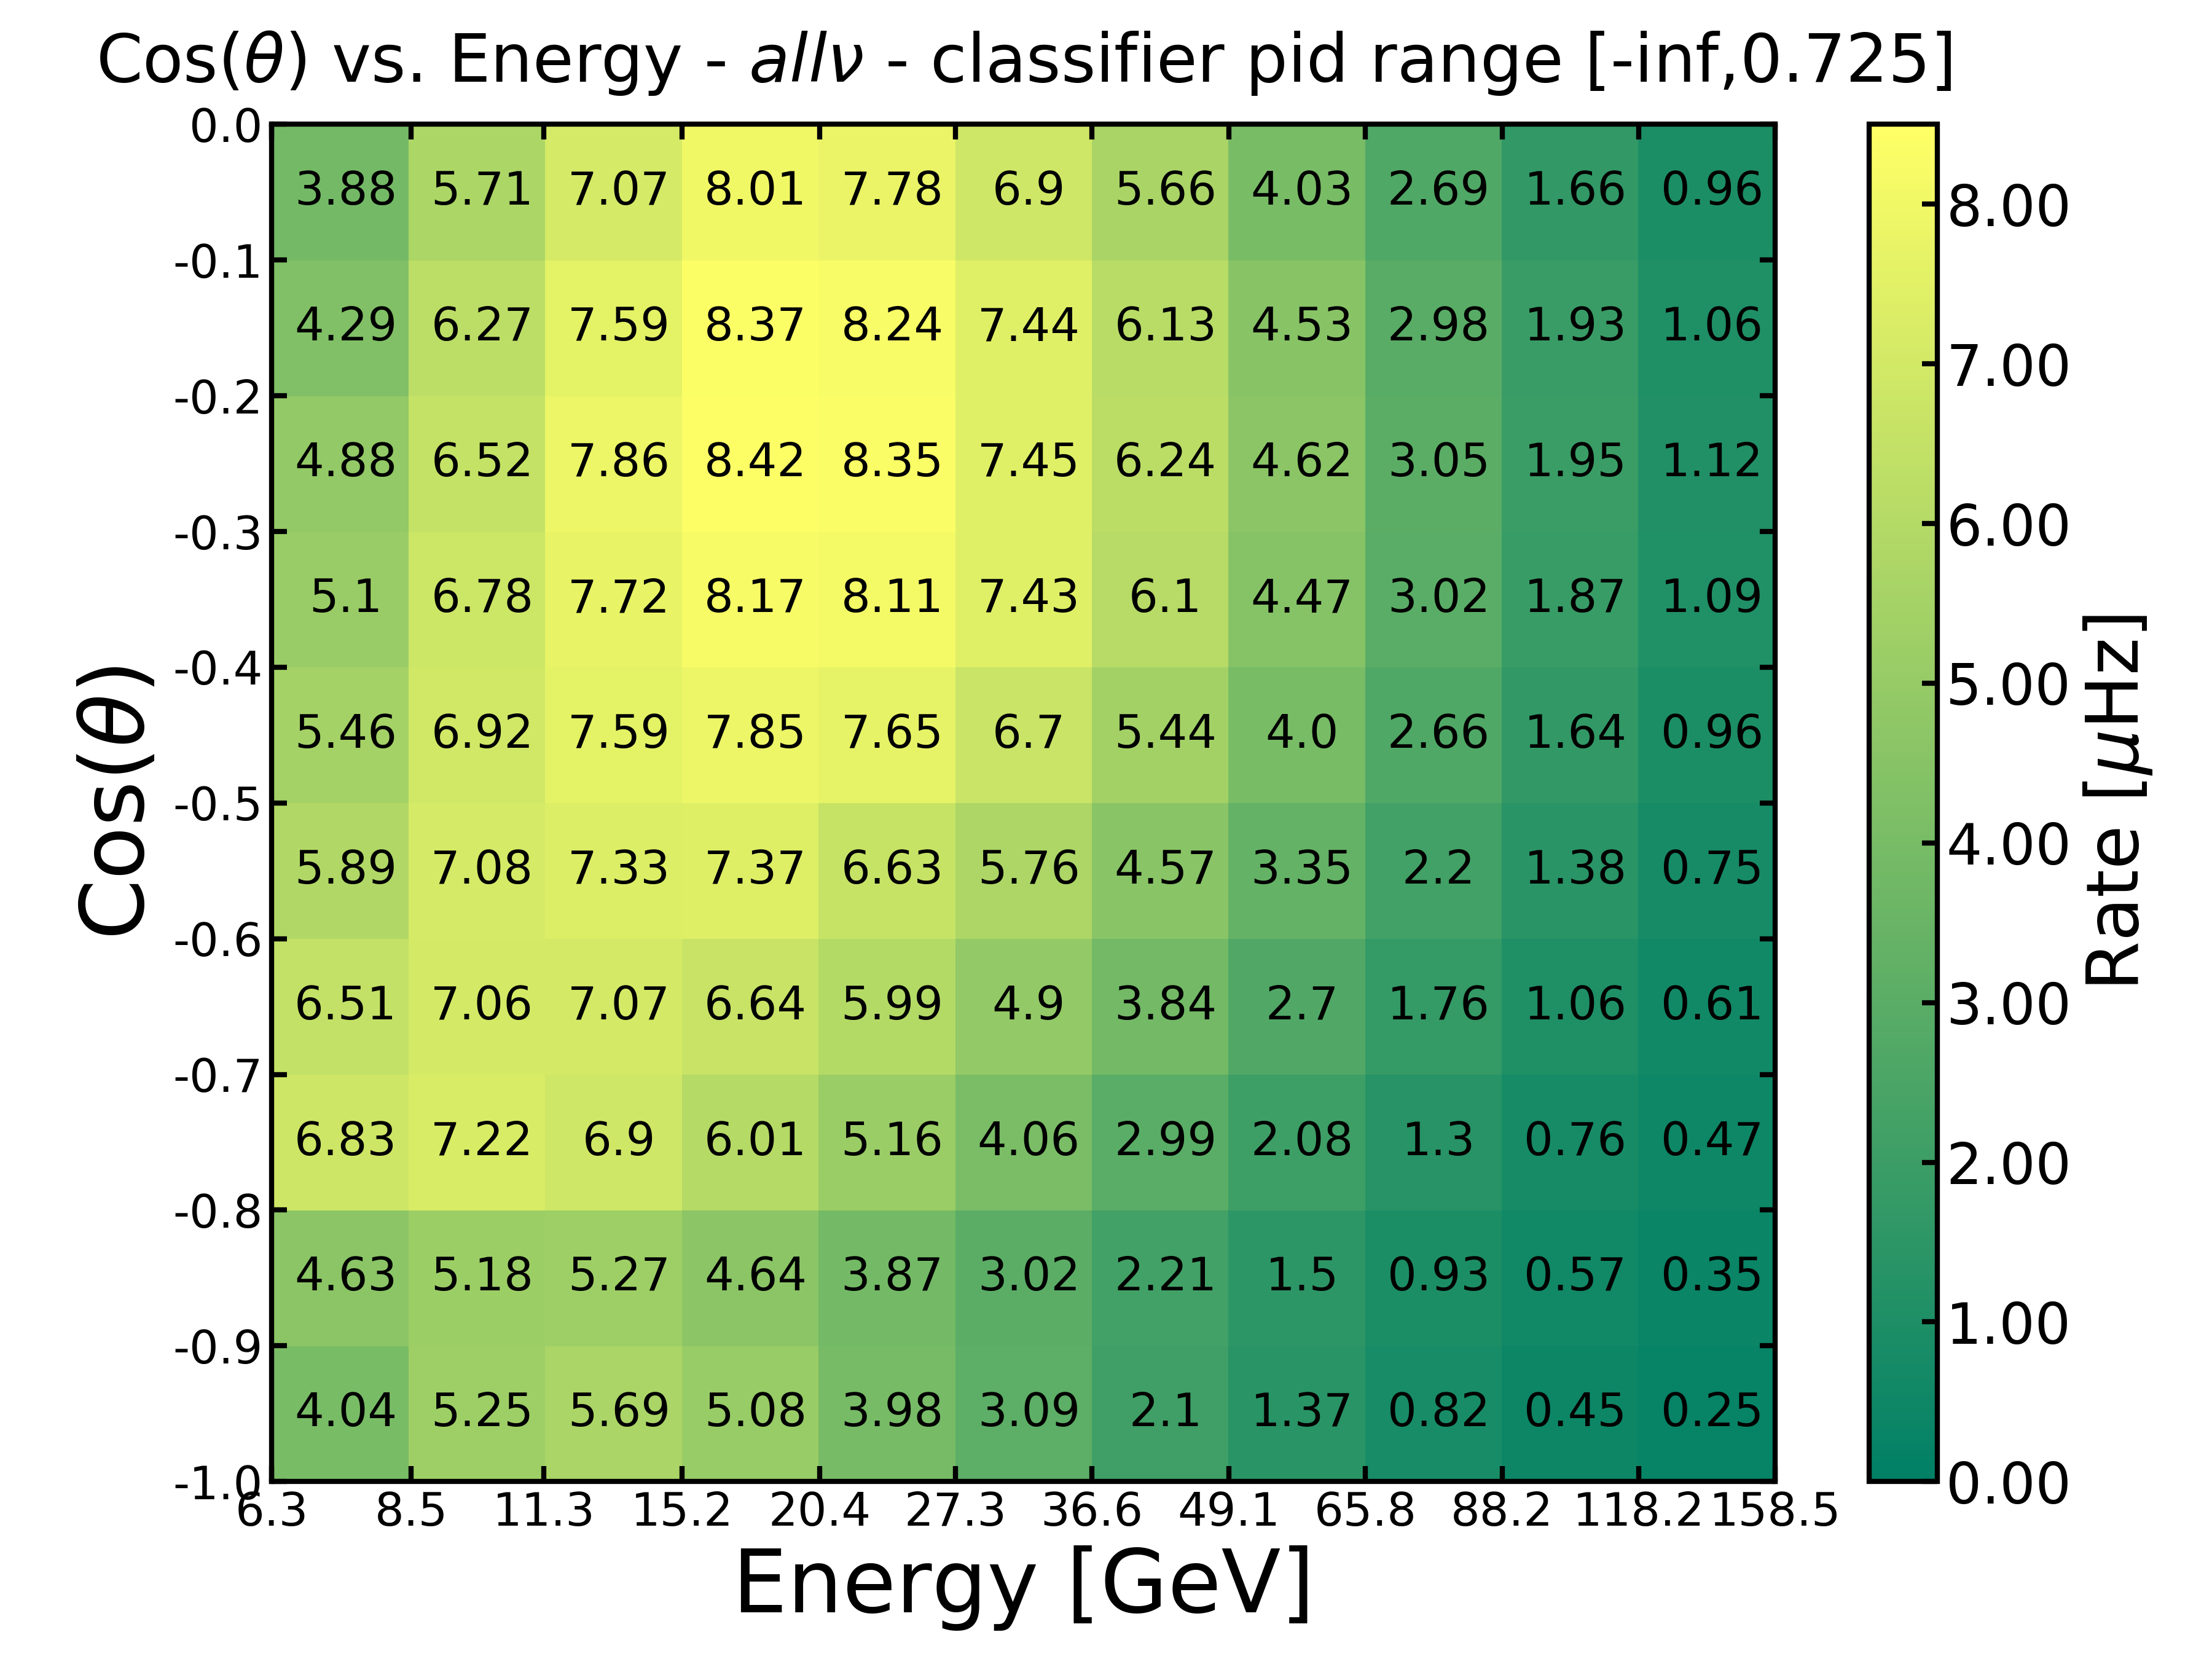
\includegraphics[width=0.49\linewidth]{figures/two_bin_cut_0725_allnu_0_oscillated_vmax.png}
    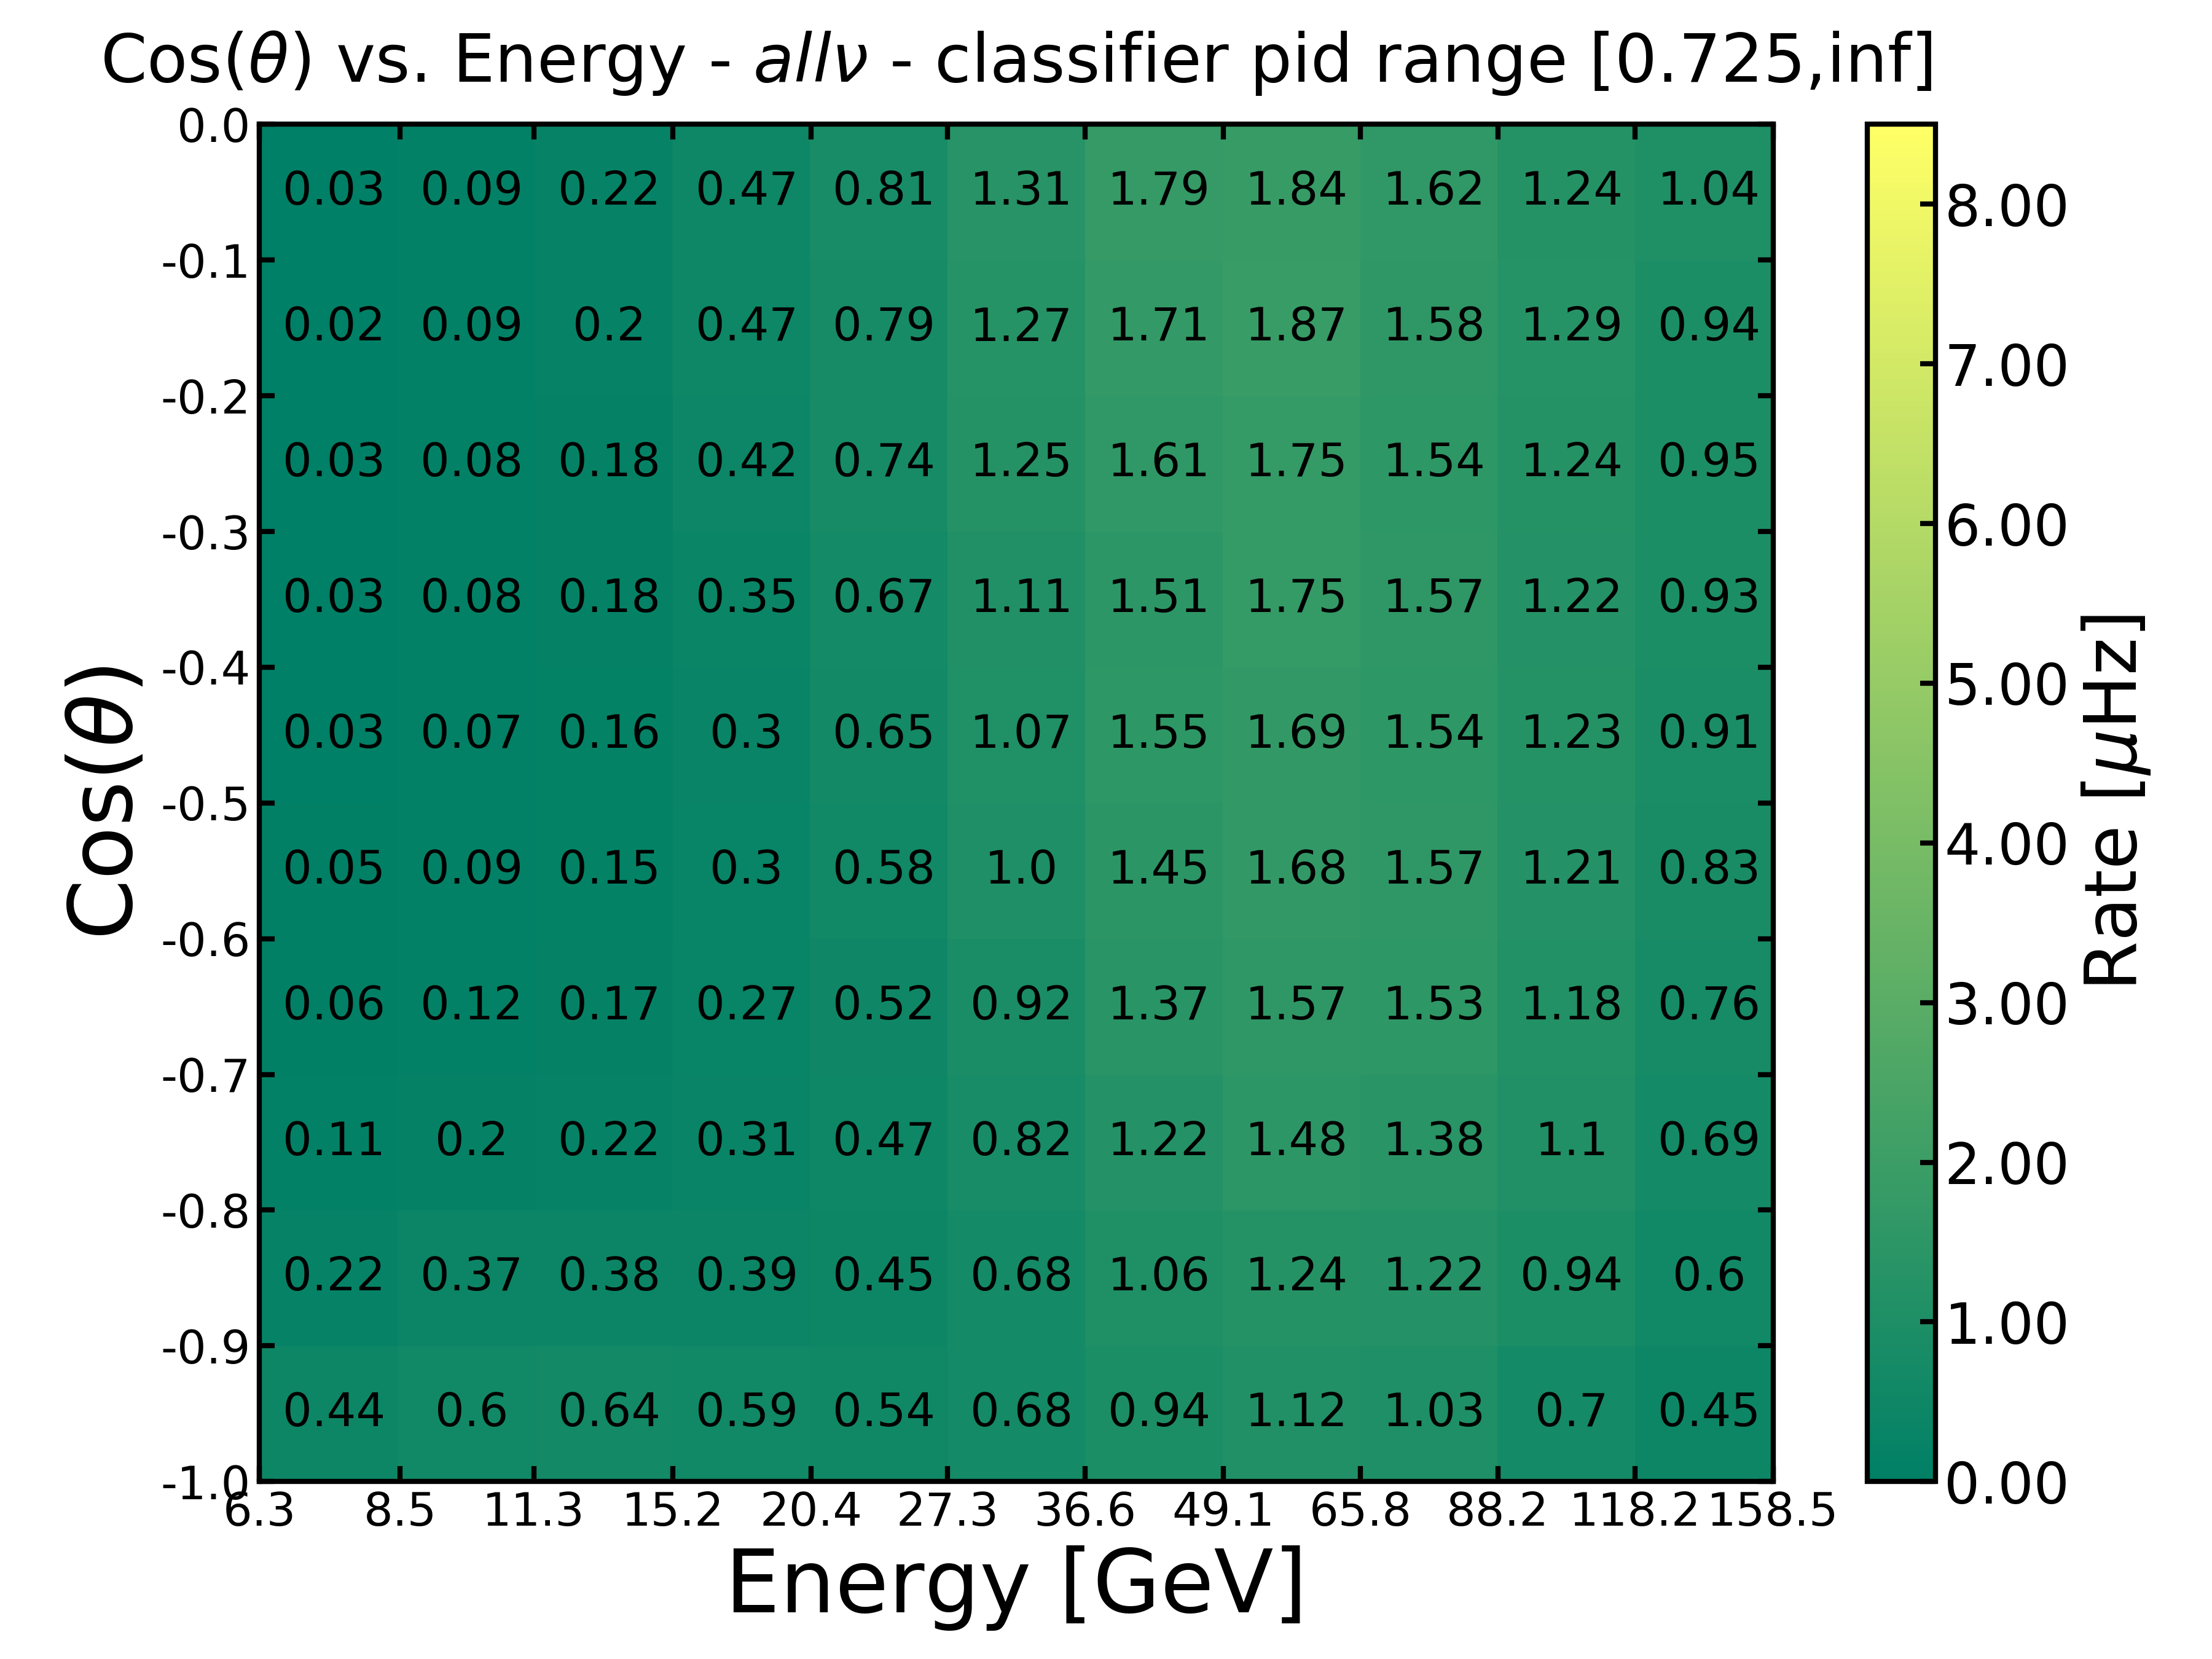
\includegraphics[width=0.49\linewidth]{figures/two_bin_cut_0725_allnu_1_oscillated_vmax.png}
    \caption[Expected oscillated event rates for two-bin case with classifier PID]{Expected oscillated event rates for two-bin case with classifier PID.}
    \label{fig:oscillated_histrograms_classifier_2bin}
\end{figure}

\begin{figure}[h]
    \centering
    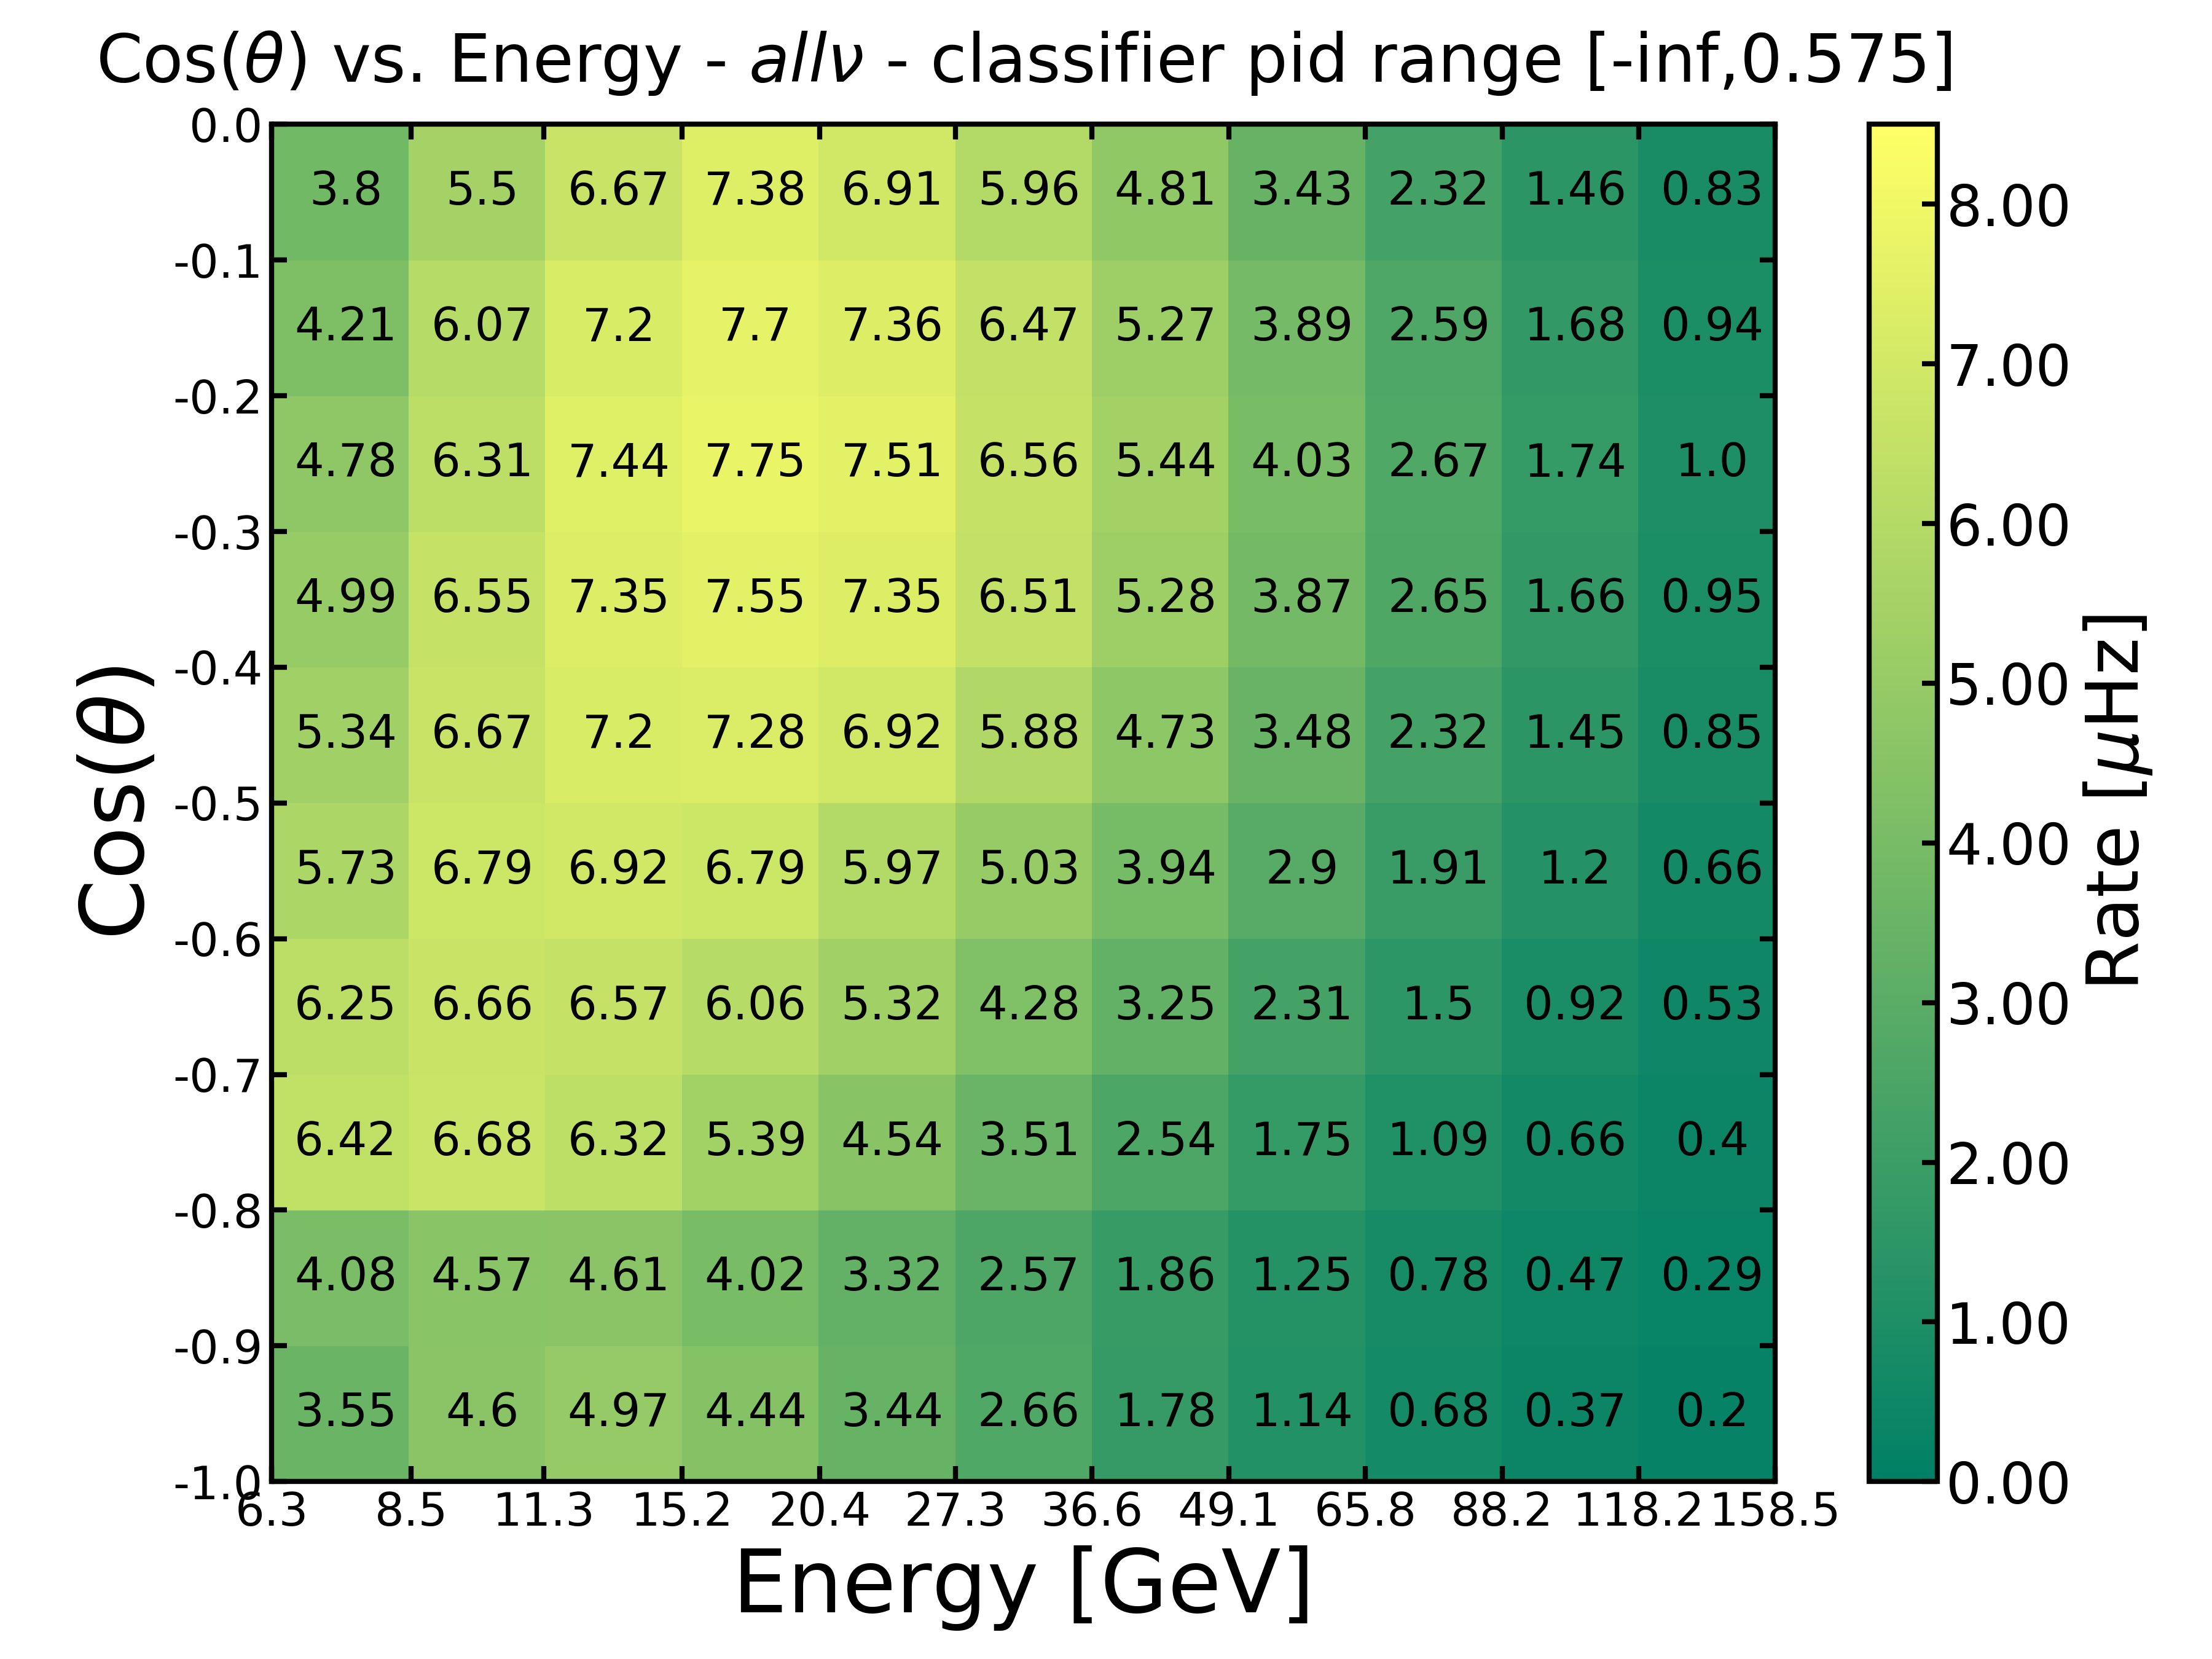
\includegraphics[width=0.49\linewidth]{figures/three_bin_cut_0575_0825_allnu_0_oscillated_vmax.png}
    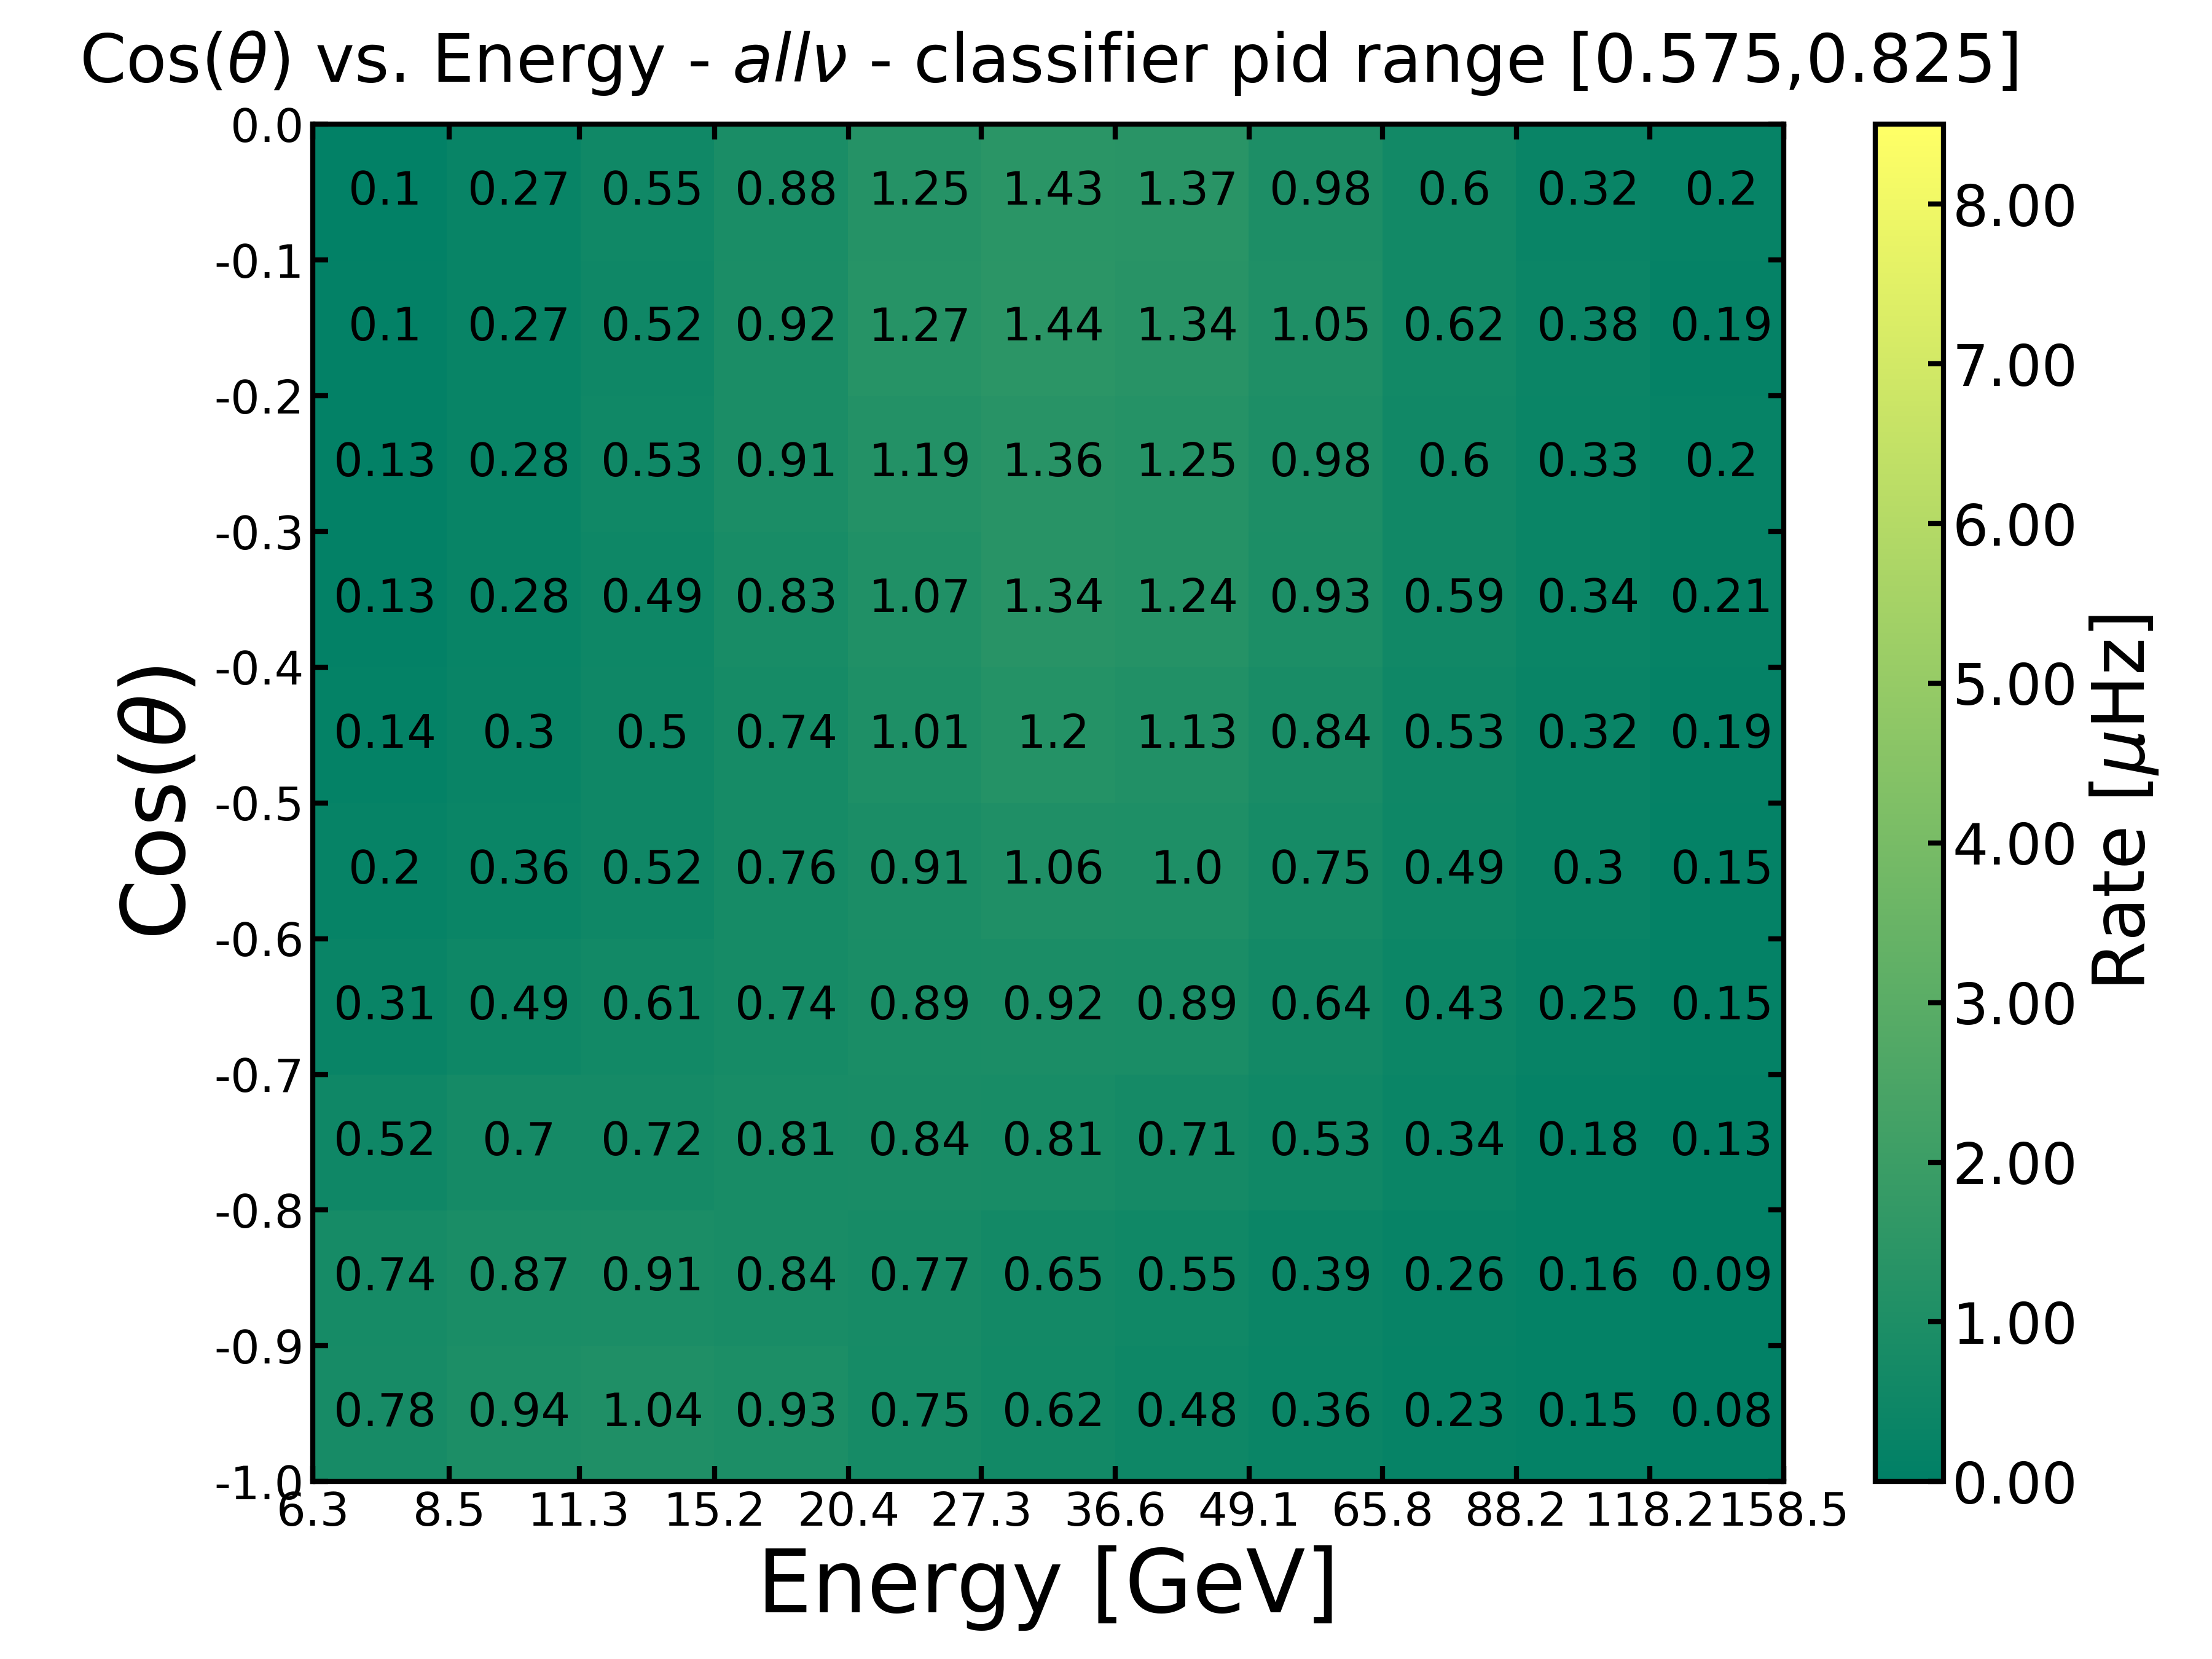
\includegraphics[width=0.49\linewidth]{figures/three_bin_cut_0575_0825_allnu_1_oscillated_vmax.png}
    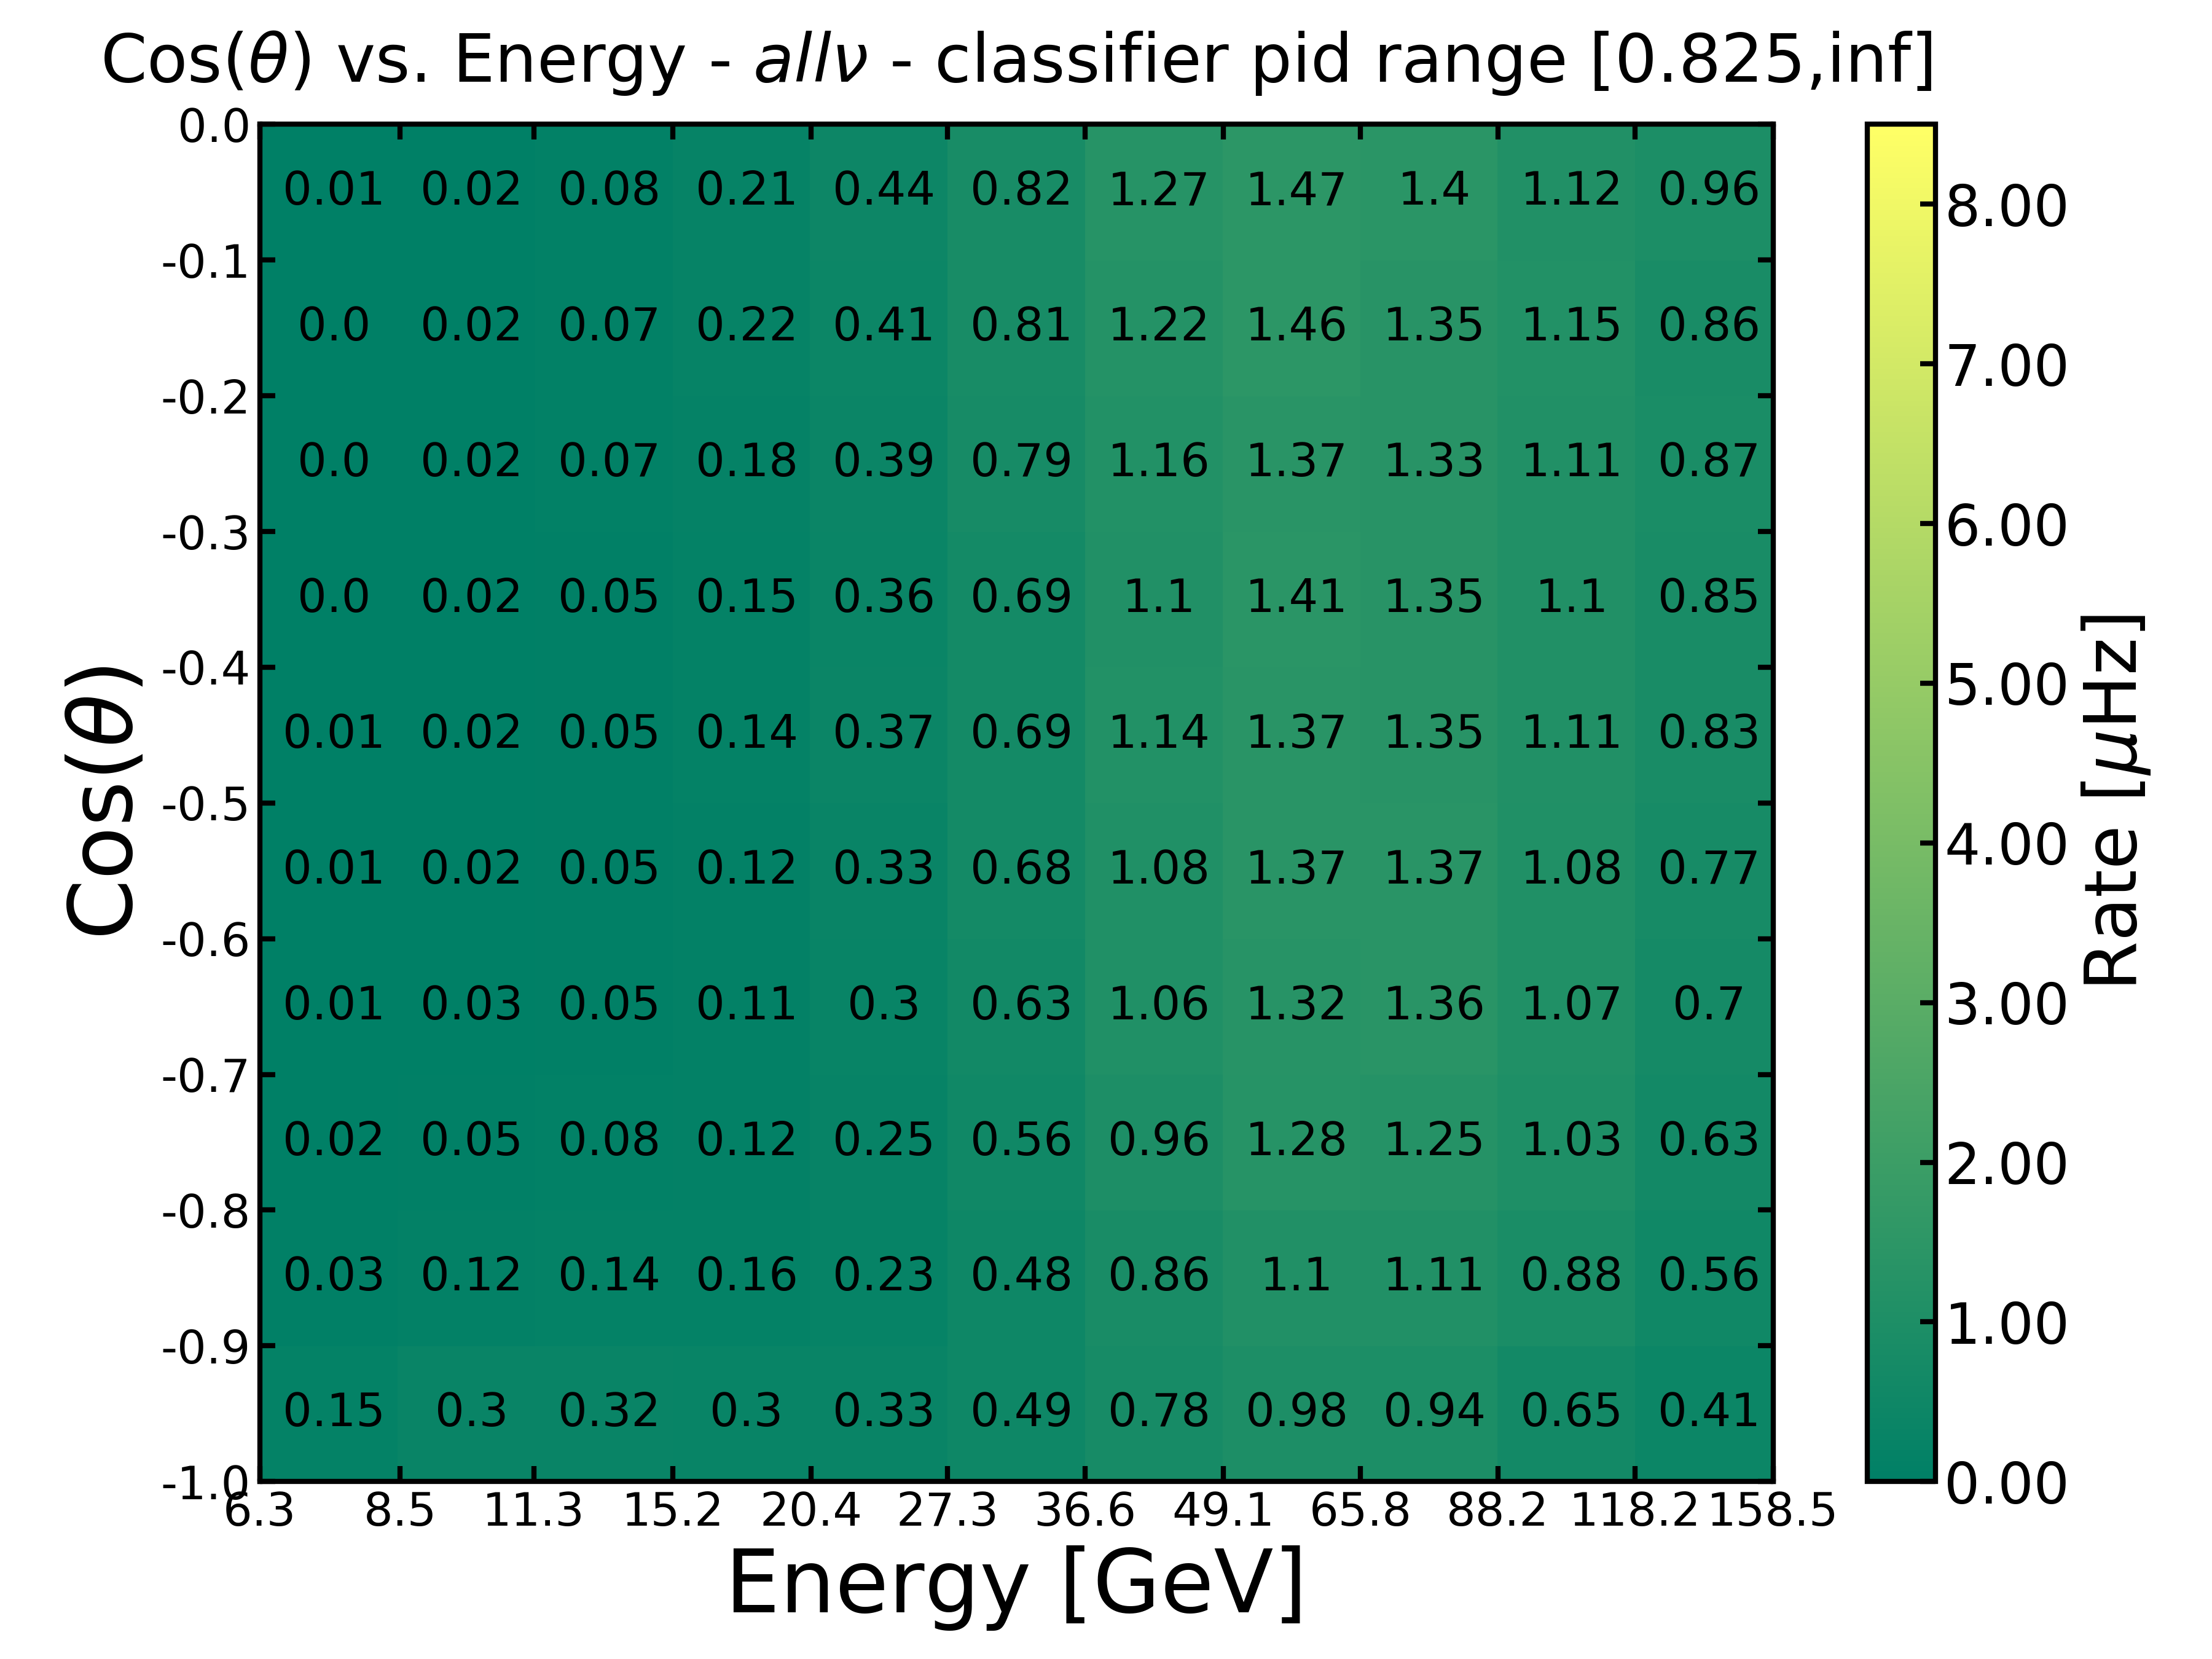
\includegraphics[width=0.49\linewidth]{figures/three_bin_cut_0575_0825_allnu_2_oscillated_vmax.png}
    \caption[Expected oscillated event rates for three-bin case with classifier PID]{Expected oscillated event rates for three-bin case with classifier PID.}
    \label{fig:oscillated_histrograms_classifier_3bin}
\end{figure}

% \begin{figure}[h]
%     \centering
%     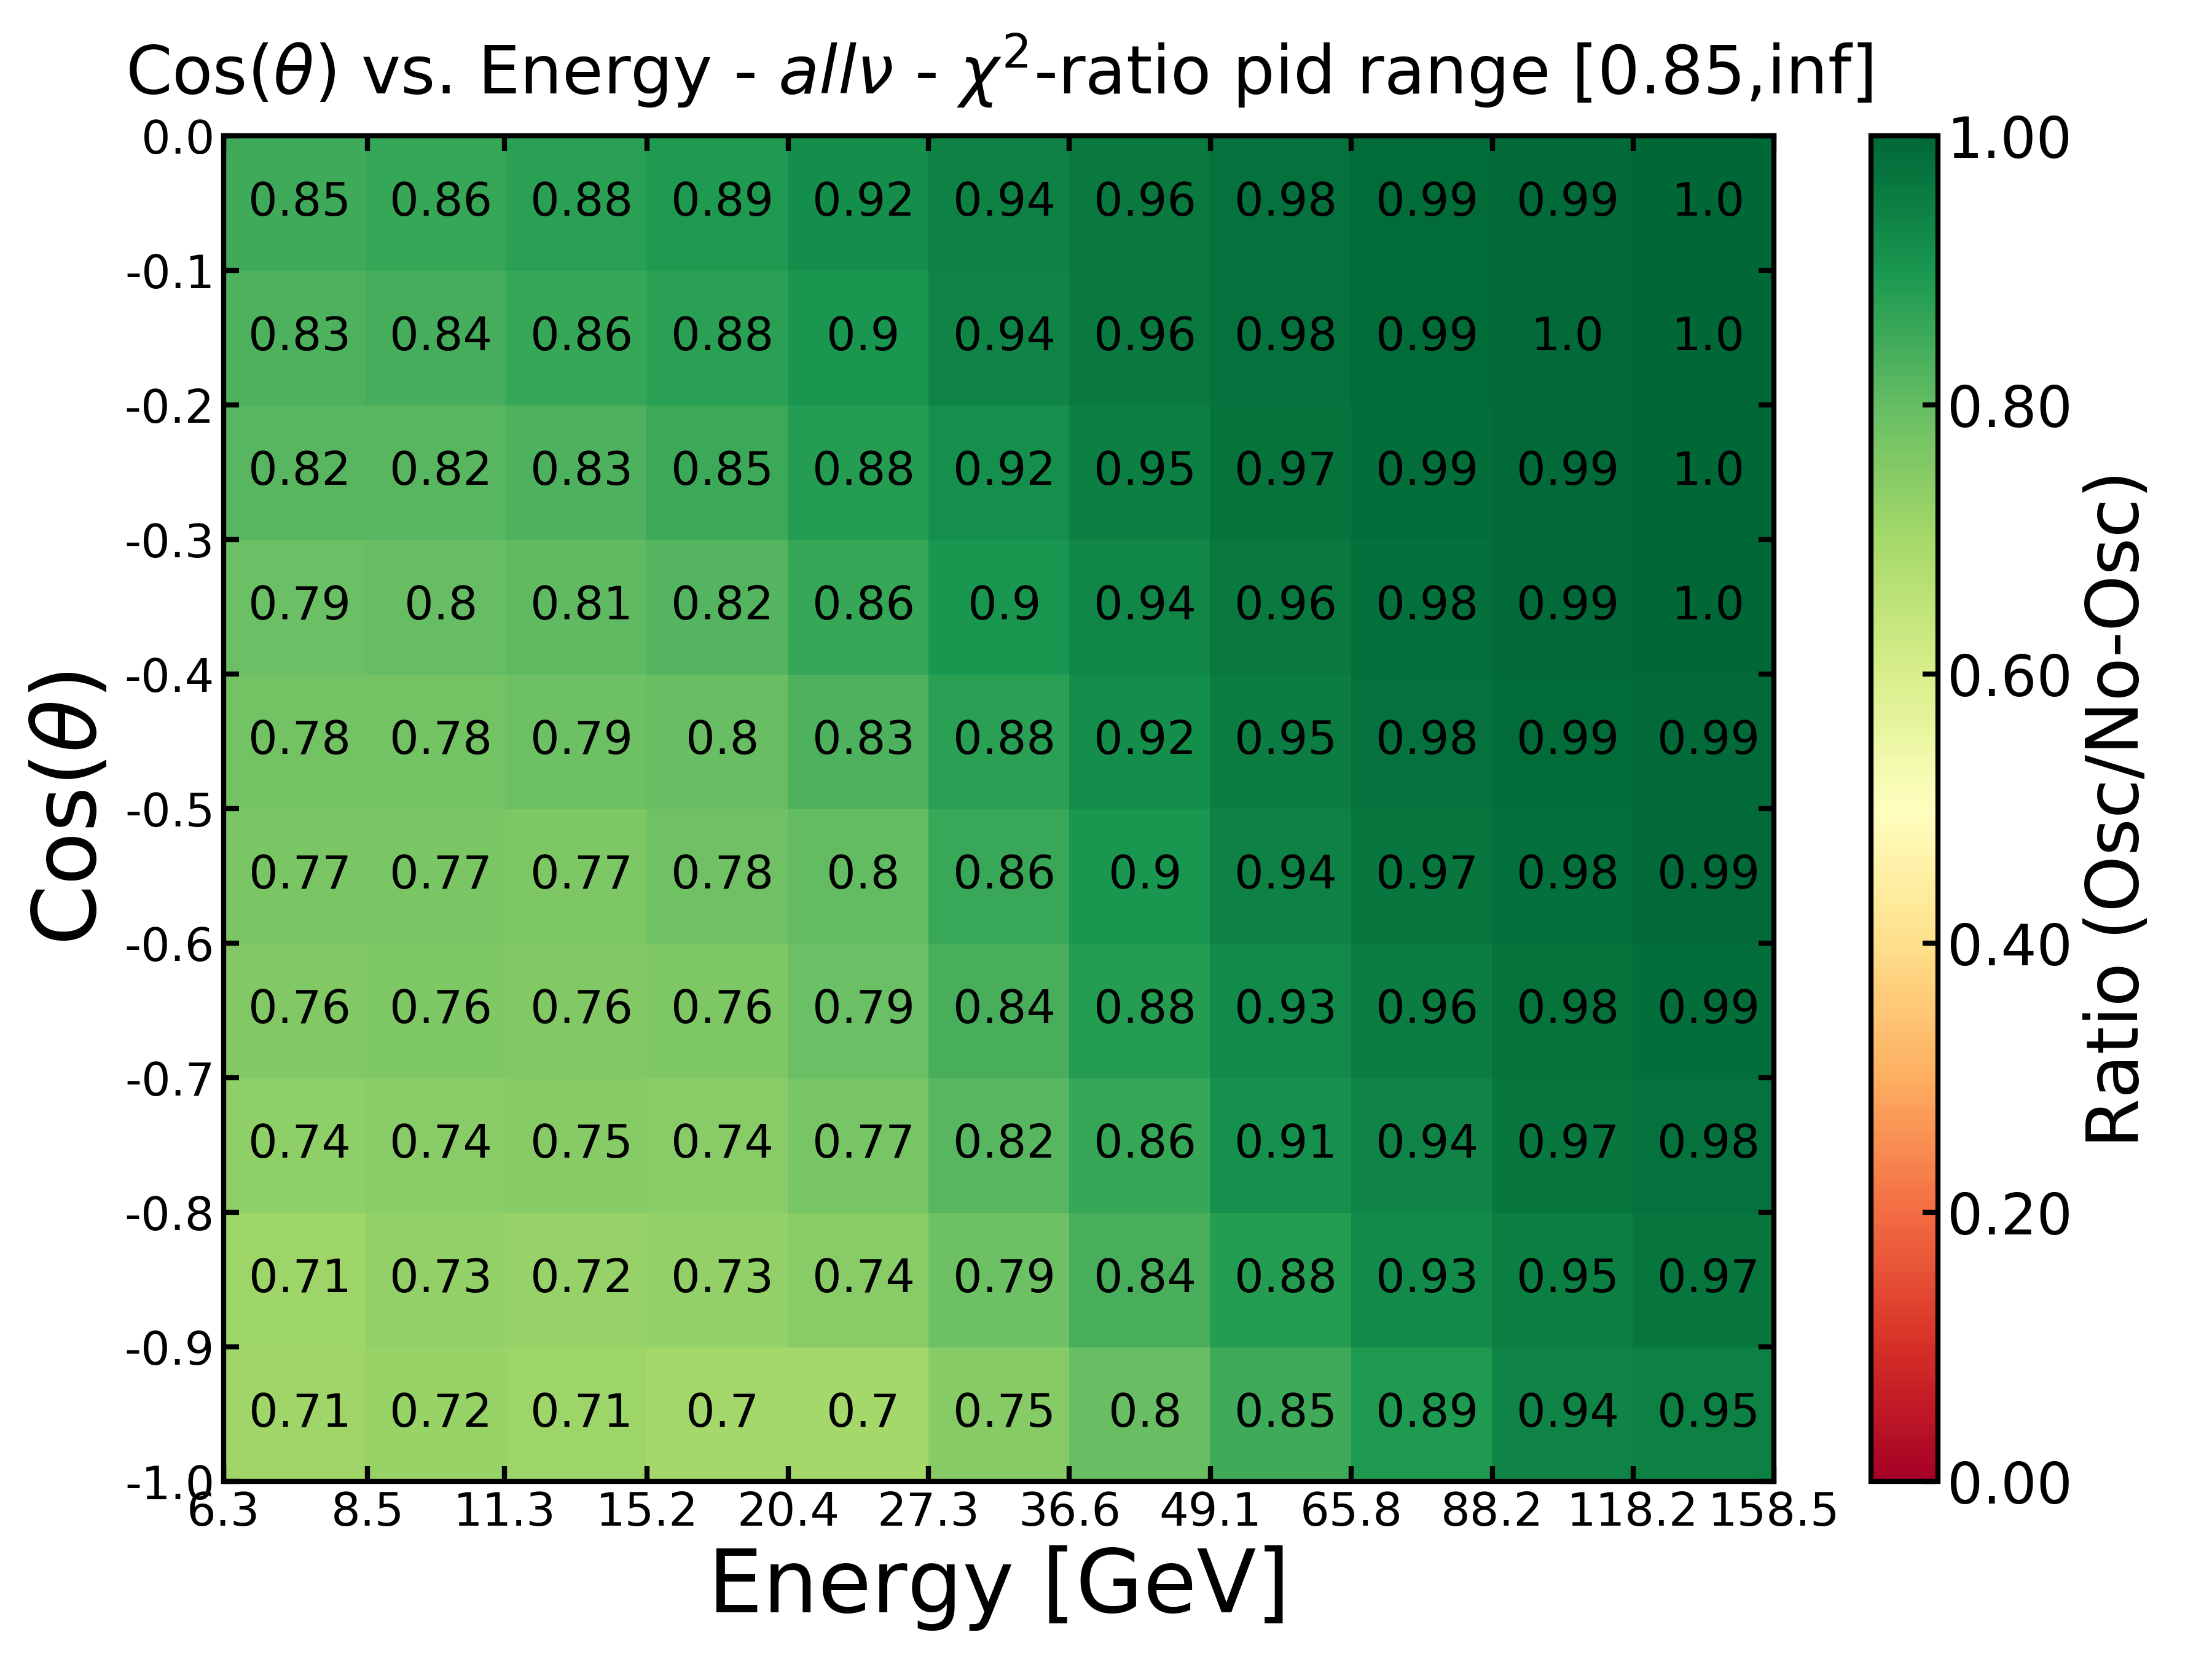
\includegraphics[width=0.49\linewidth]{figures/santa_cut_085_allnu_1_ratio_osc_noosc.png}
%     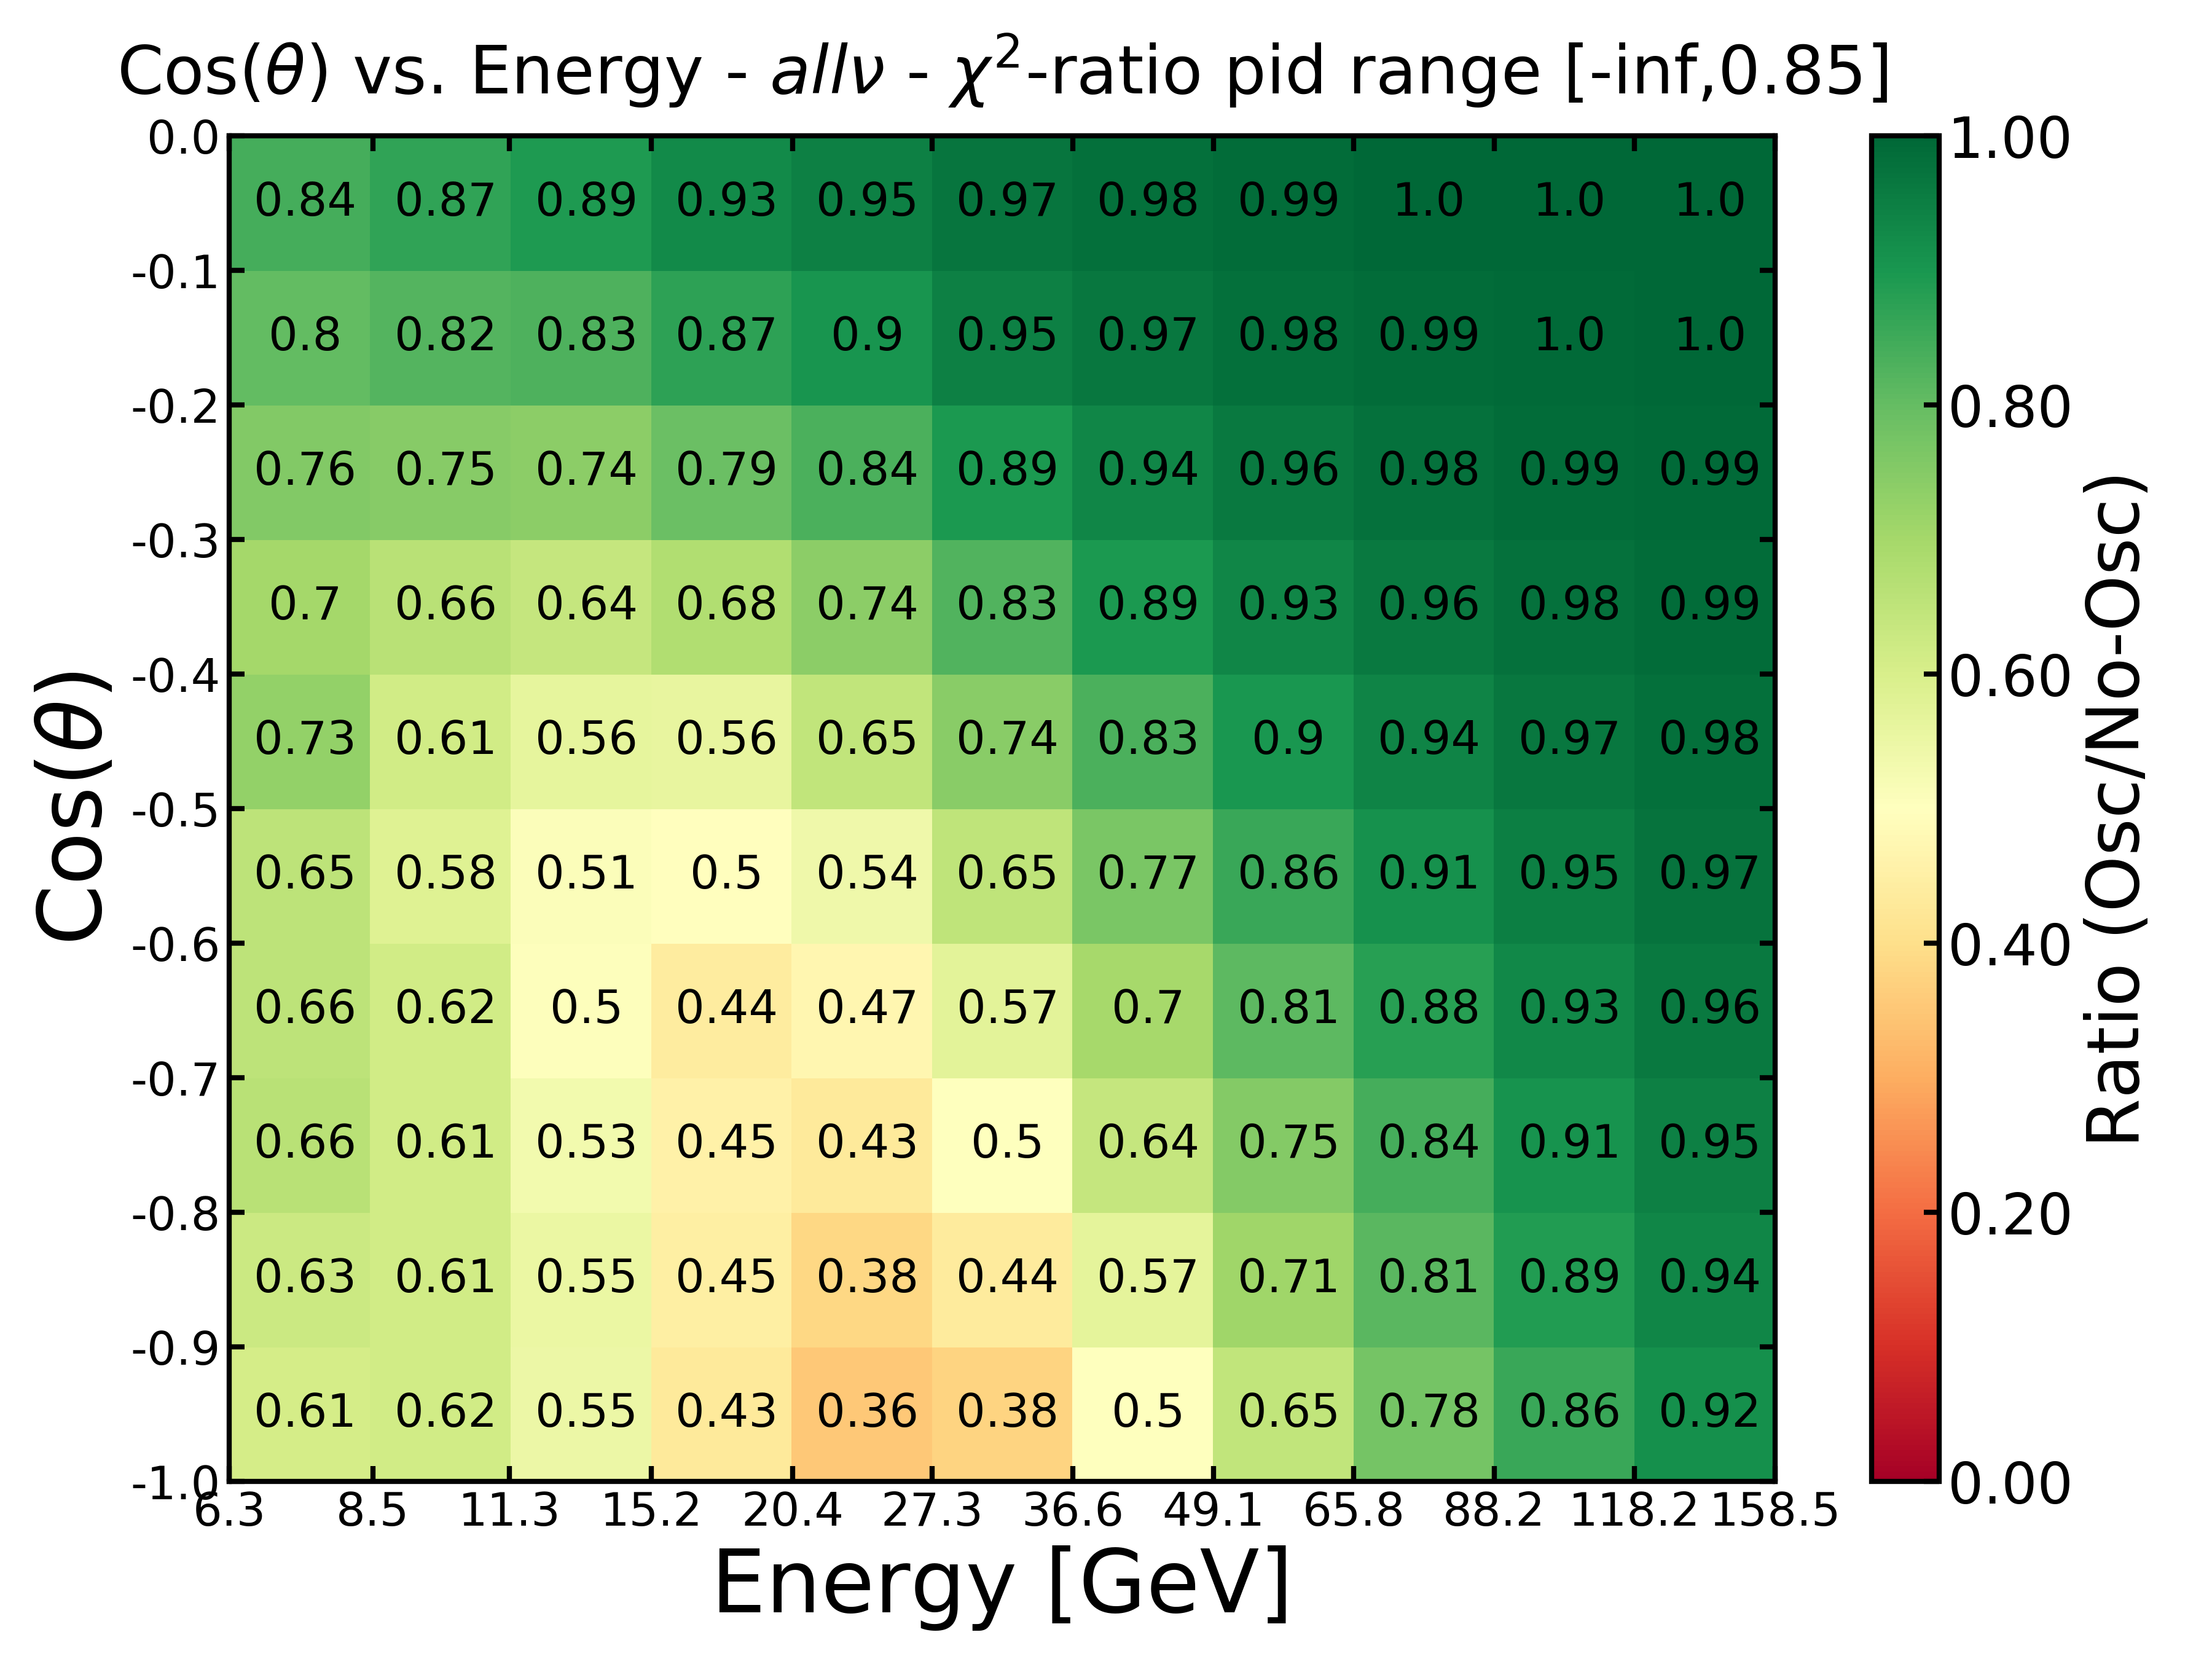
\includegraphics[width=0.49\linewidth]{figures/santa_cut_085_allnu_0_ratio_osc_noosc.png}
%     \caption[Expected neutrino oscillation effects for two-bin case with $\chi^2\textrm{-ratio}$ PID]{Expected neutrino oscillation effects for two-bin case with $\chi^2\textrm{-ratio}$ PID. Shown is the ration between unoscillated and oscillated event rates.}
%     \label{fig:xx}
% \end{figure}

% \begin{figure}[h]
%     \centering
%     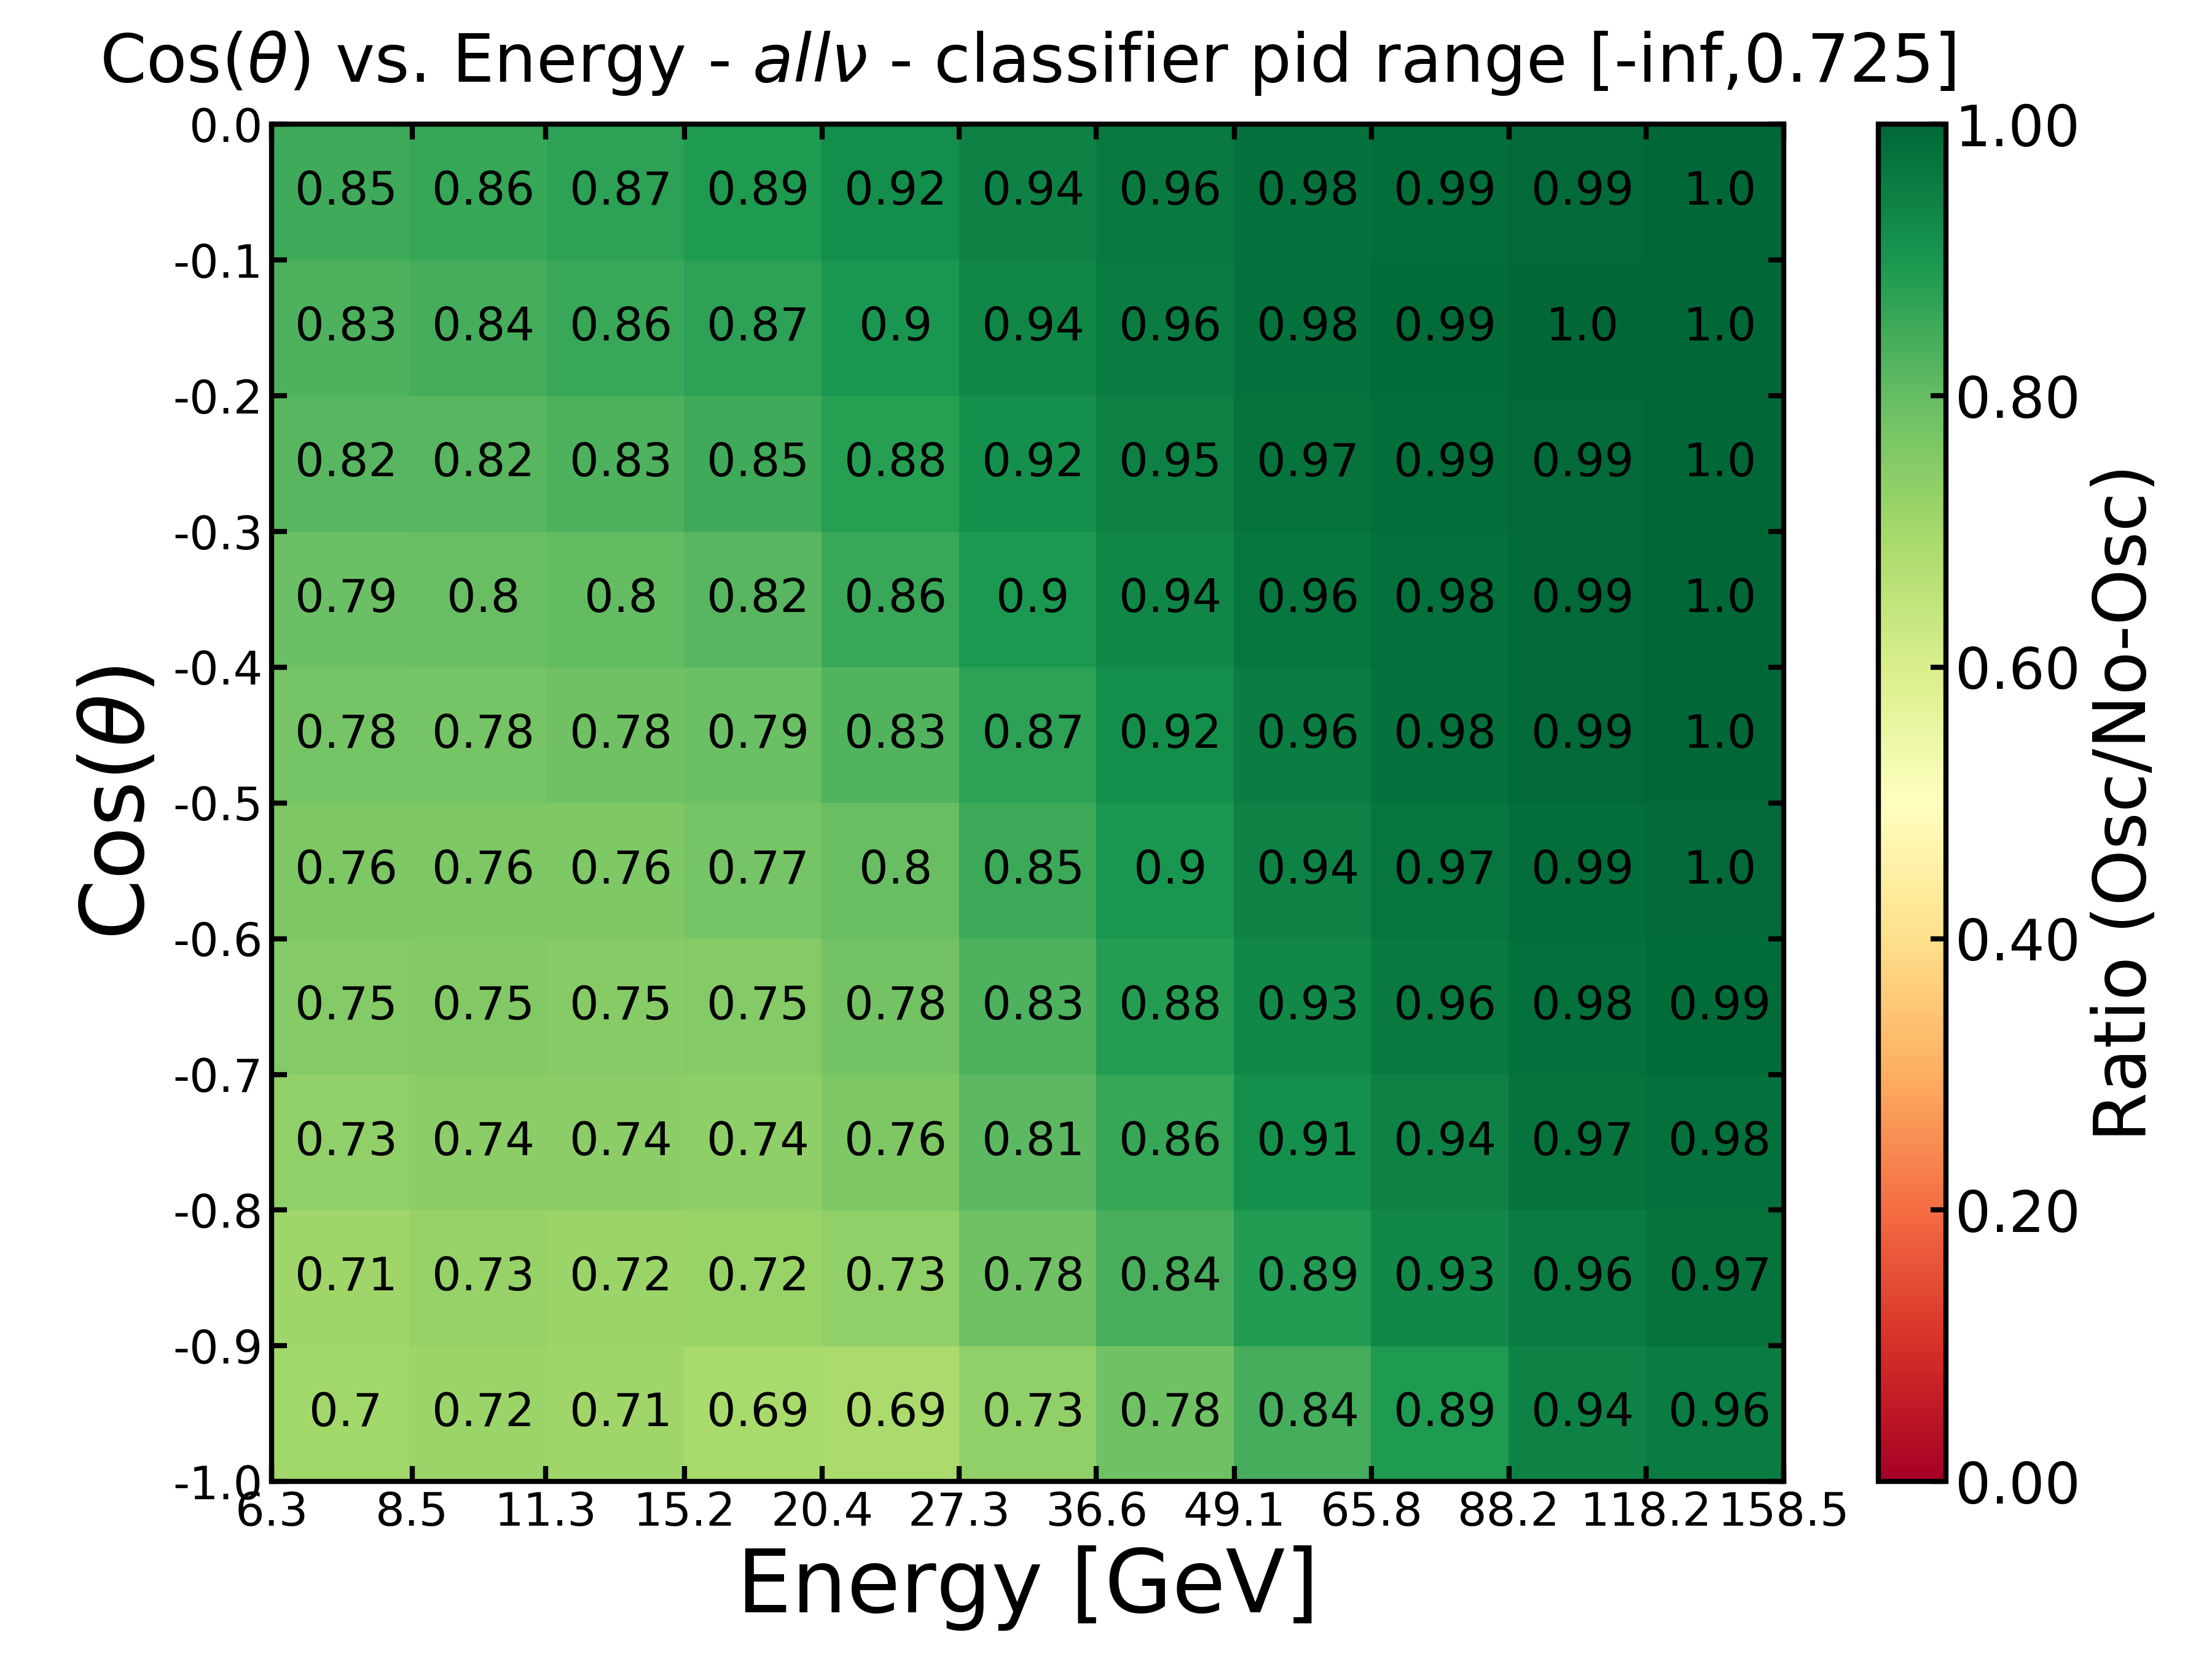
\includegraphics[width=0.49\linewidth]{figures/two_bin_cut_0725_allnu_0_ratio_osc_noosc.png}
%     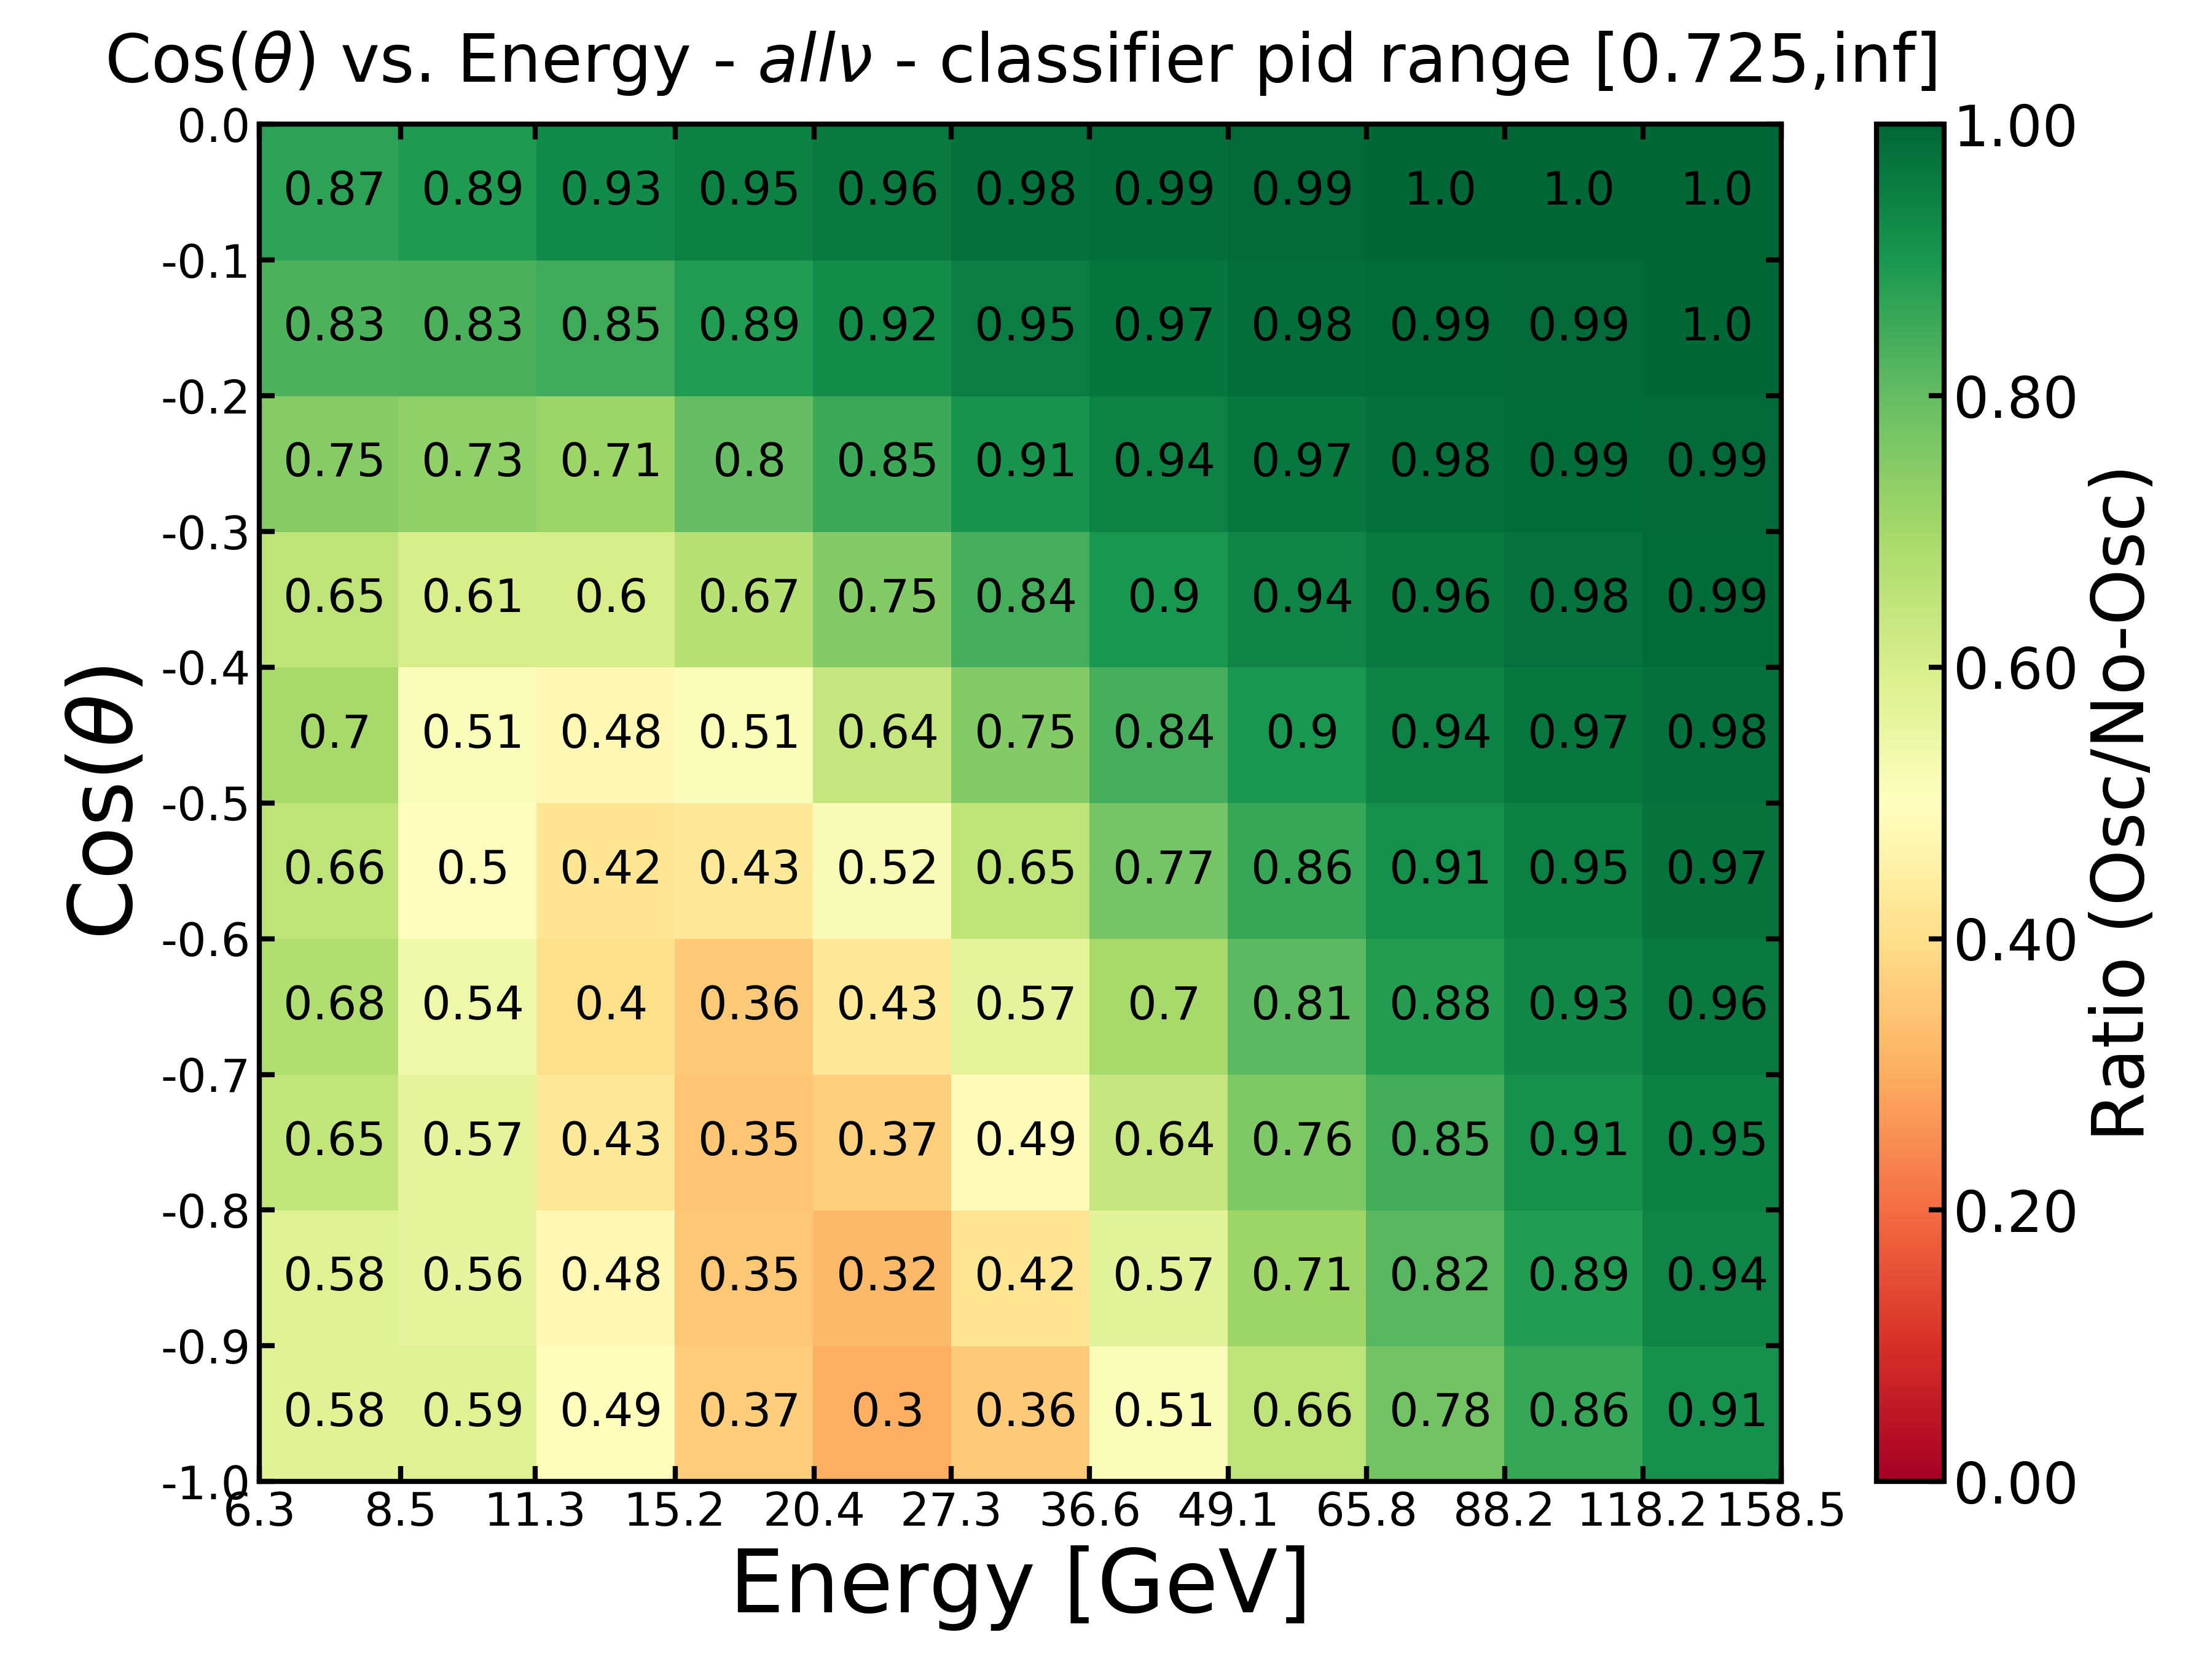
\includegraphics[width=0.49\linewidth]{figures/two_bin_cut_0725_allnu_1_ratio_osc_noosc.png}
%     \caption[Expected neutrino oscillation effects for two-bin case with classifier PID]{Expected neutrino oscillation effects for two-bin case with classifier PID. Shown is the ration between unoscillated and oscillated event rates.}
%     \label{fig:xxx}
% \end{figure}

% \begin{figure}[h]
%     \centering
%     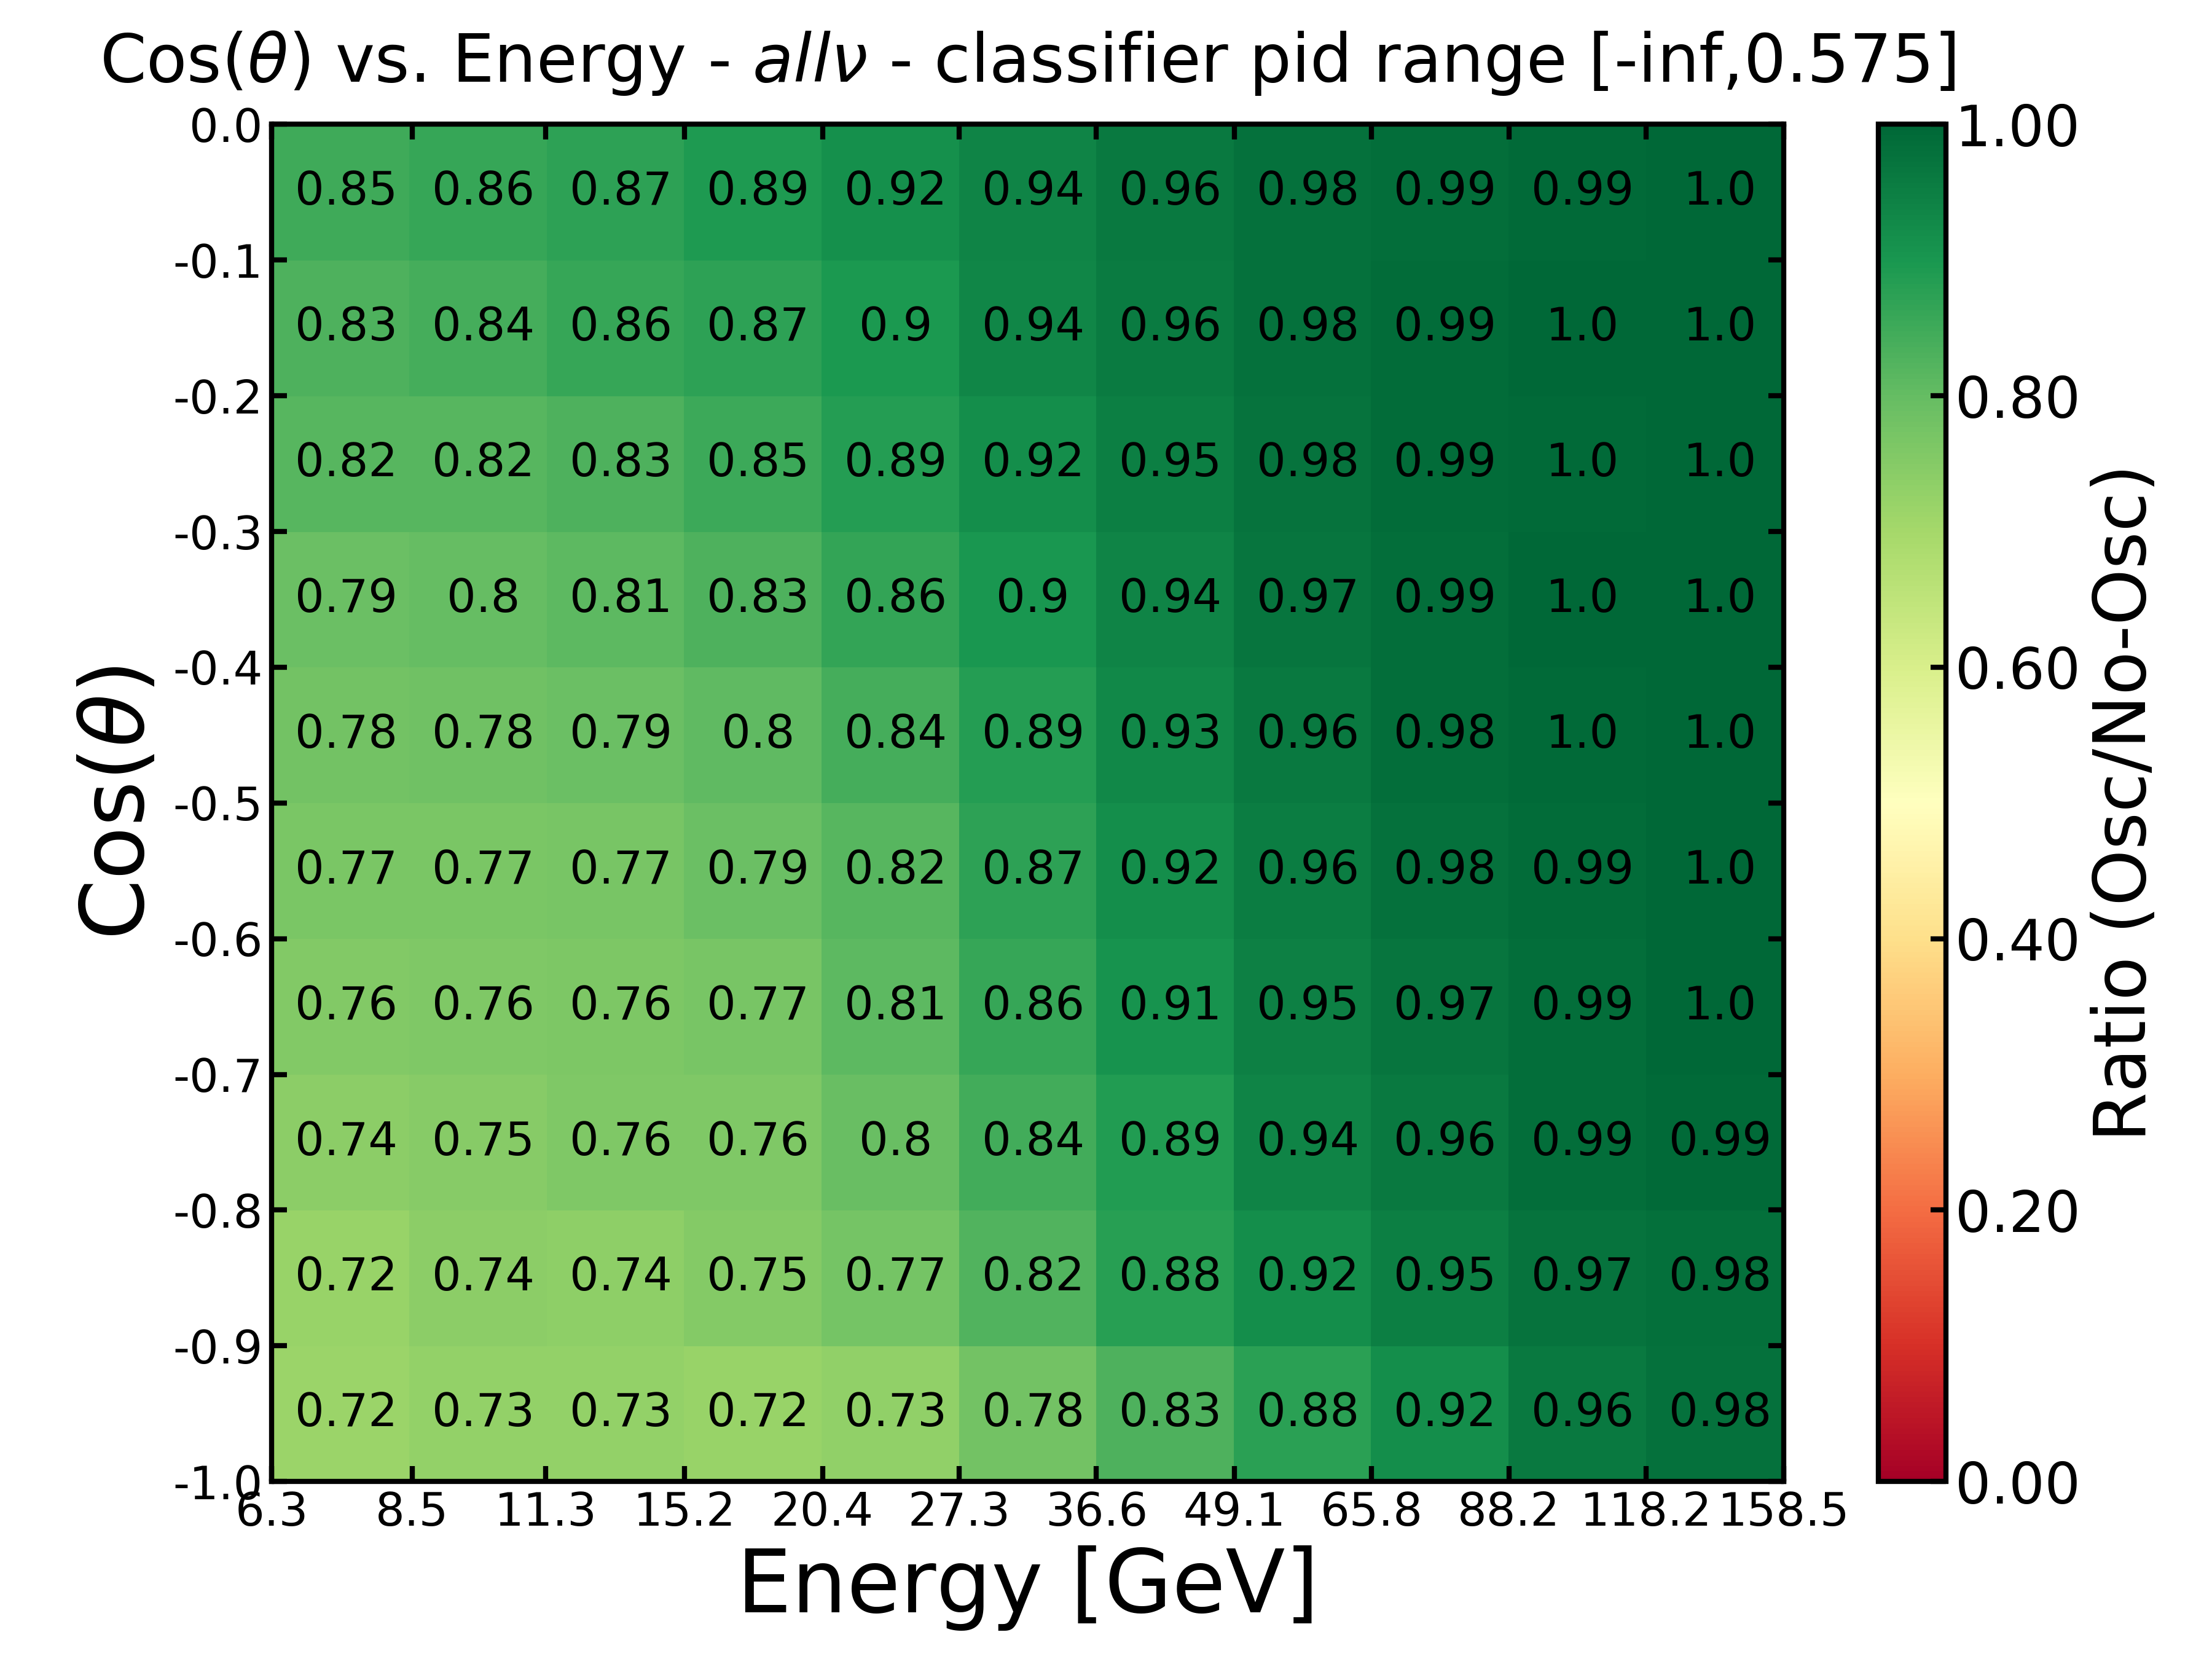
\includegraphics[width=0.49\linewidth]{figures/three_bin_cut_0575_0825_allnu_0_ratio_osc_noosc.png}
%     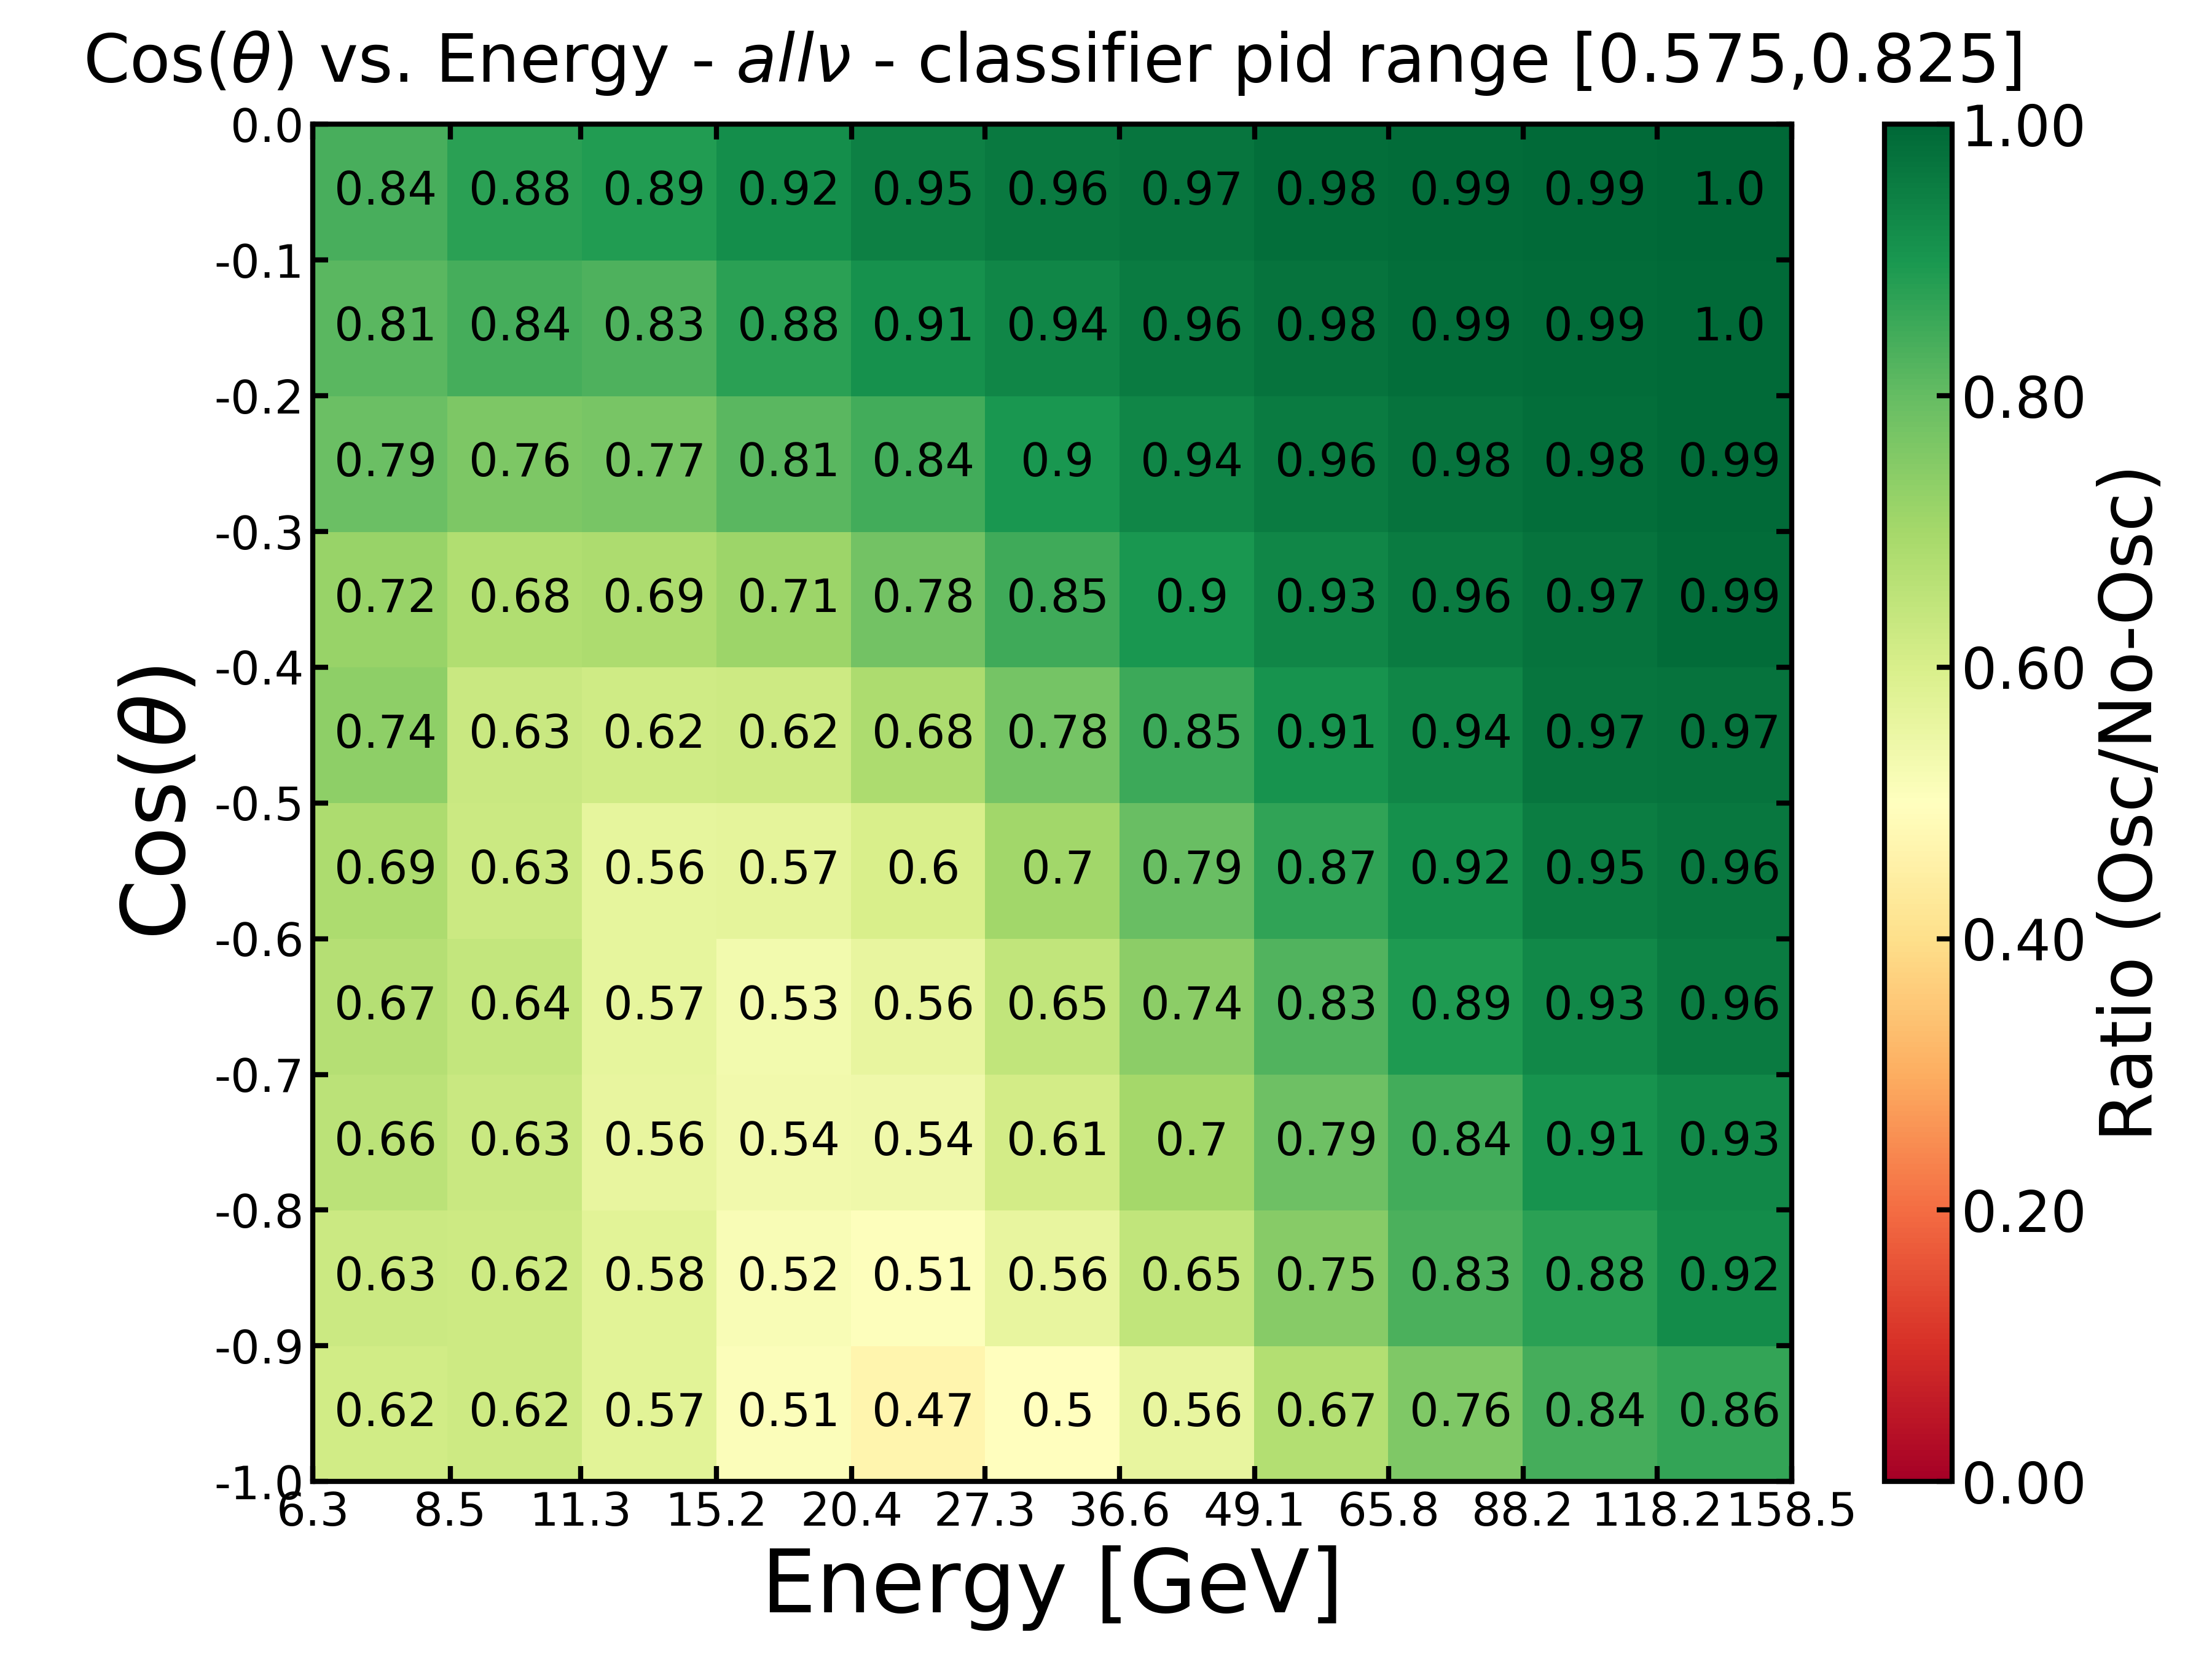
\includegraphics[width=0.49\linewidth]{figures/three_bin_cut_0575_0825_allnu_1_ratio_osc_noosc.png}
%     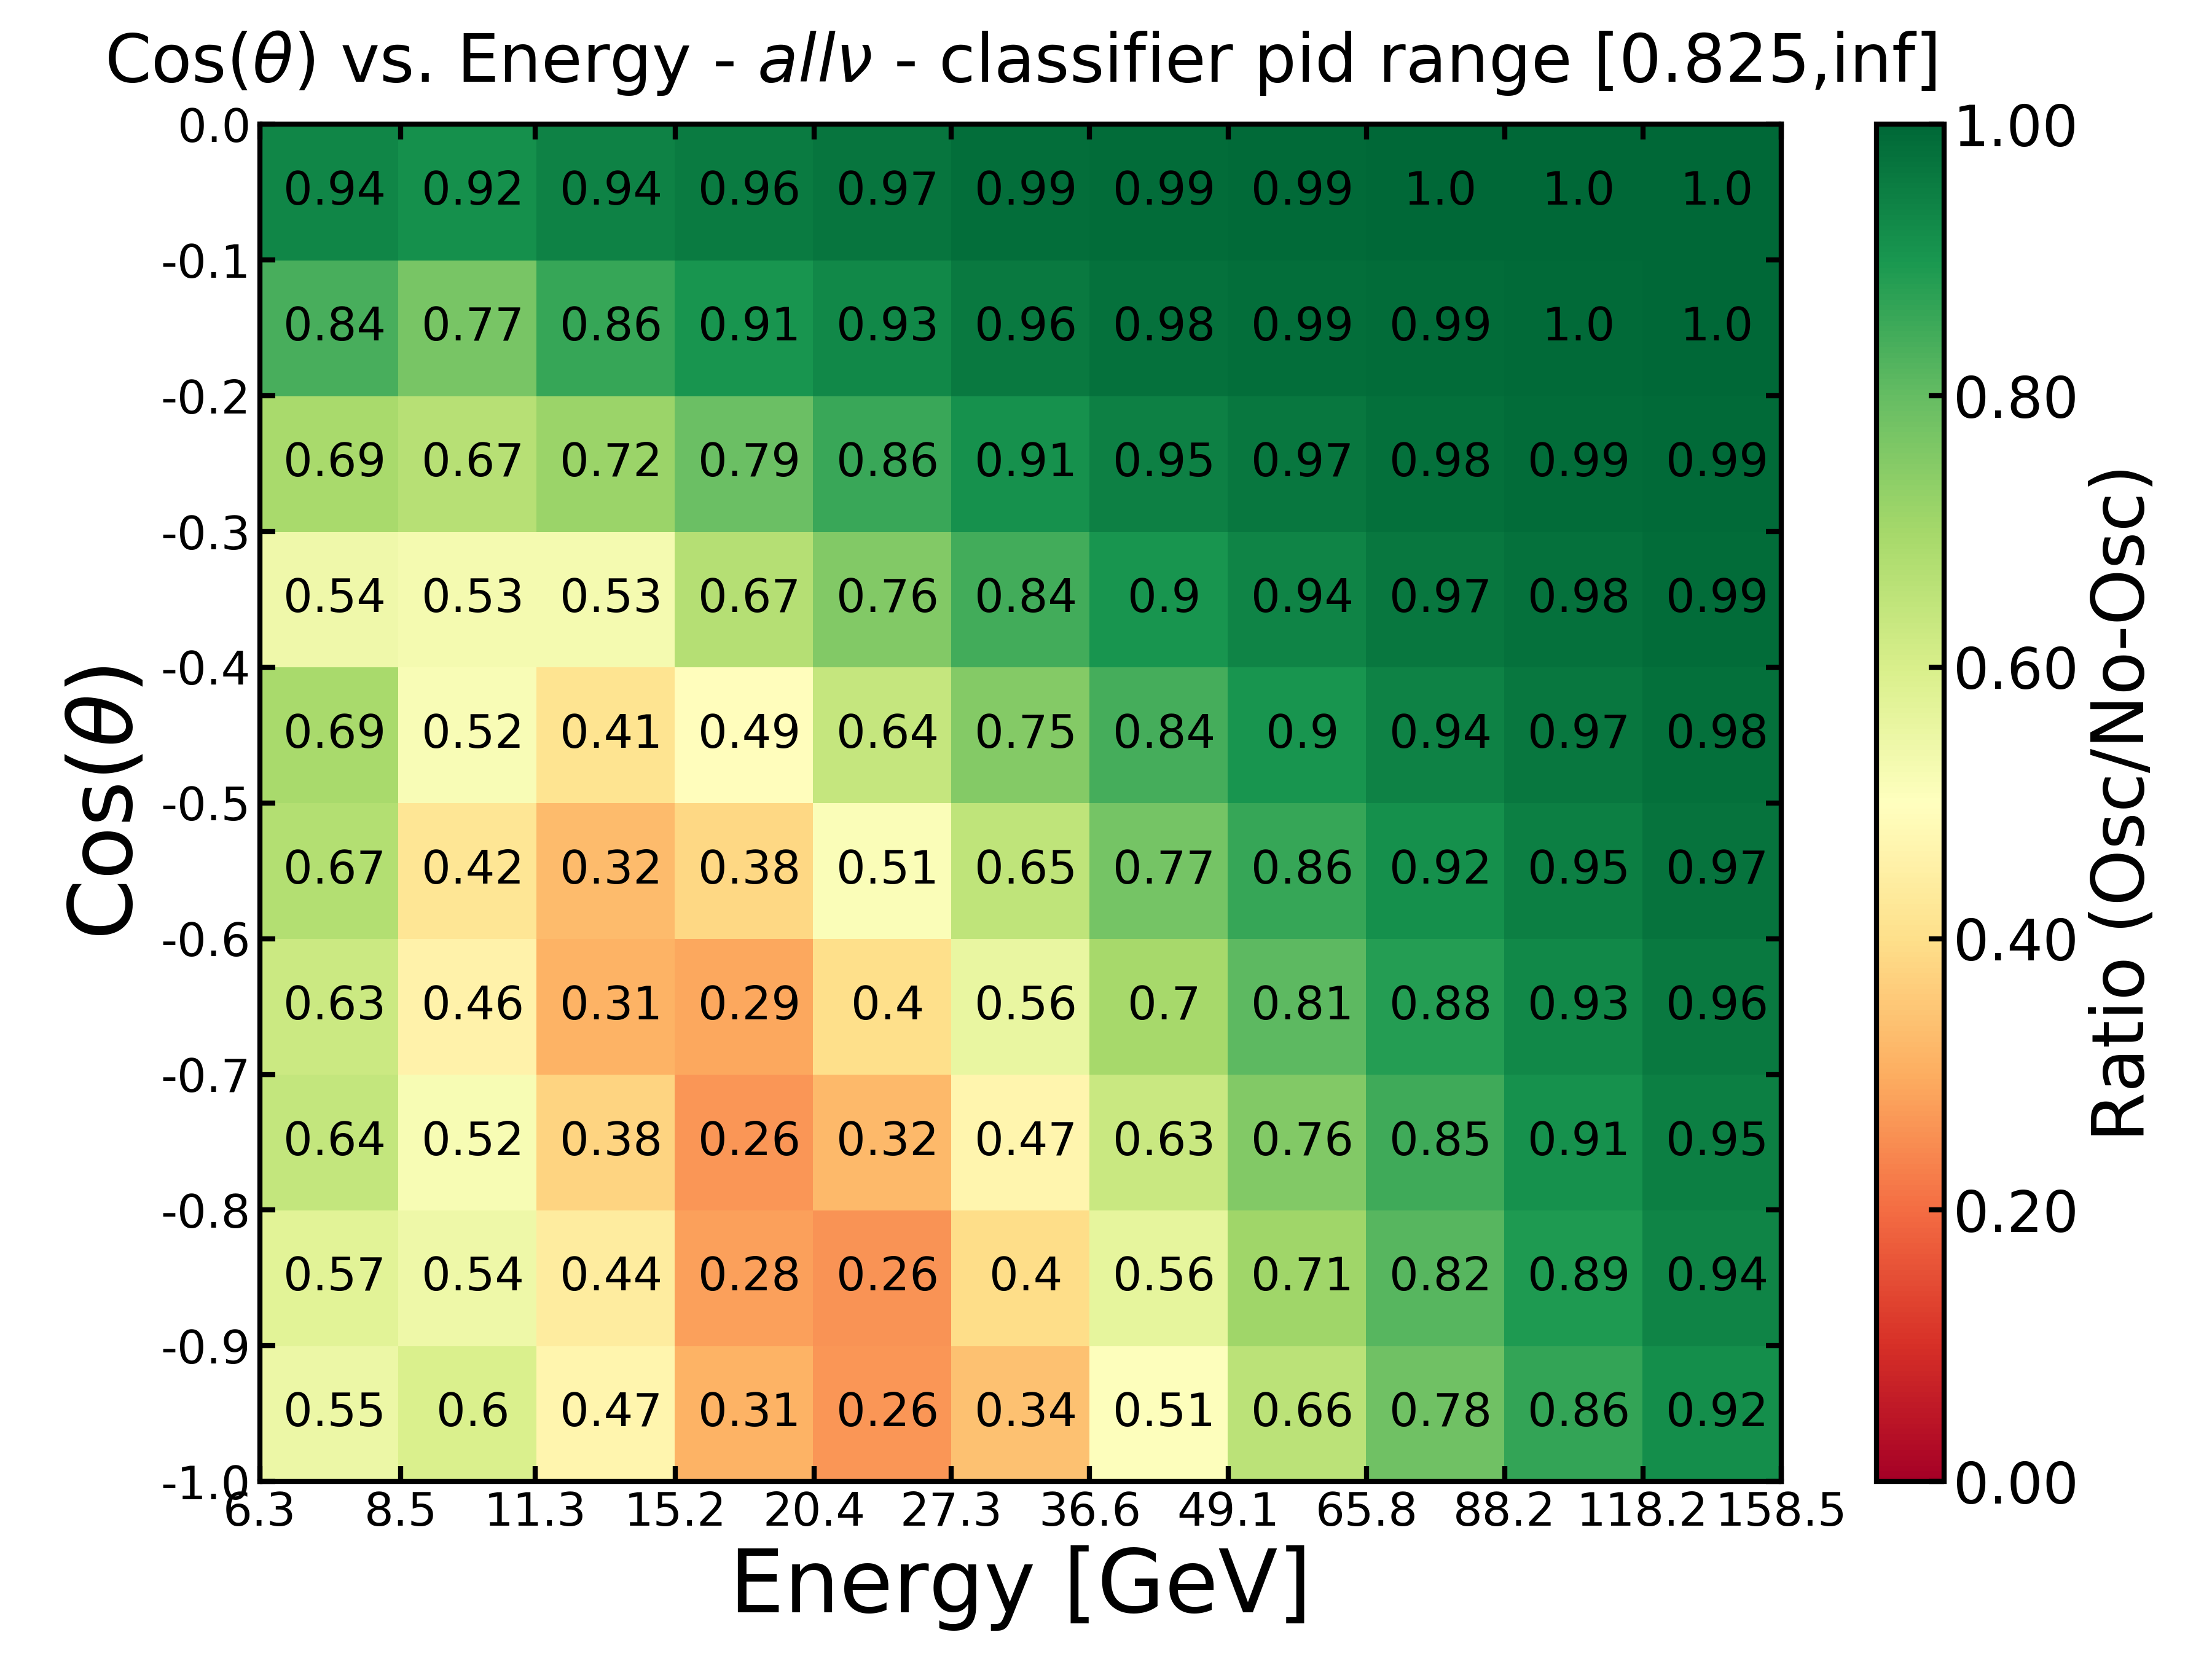
\includegraphics[width=0.49\linewidth]{figures/three_bin_cut_0575_0825_allnu_2_ratio_osc_noosc.png}
%     \caption[Expected neutrino oscillation effects for three-bin case with classifier PID]{Expected neutrino oscillation effects for three-bin case with classifier PID. Shown is the ration between unoscillated and oscillated event rates.}
%     \label{fig:xxxx}
% \end{figure}

\end{appendices}